\chapter{Analyse}\label{analyse}

\section{Vorgehen und Zielsetzung}\label{vorgehen-und-zielsetzung}

Die Analyse wird mithilfe der vorgeschlagenen Methode \emph{corpus-driven} ermittelte Frame-Strukturen\footnote{Die Visualisierungen sind unter \url{https://doi.org/10.5281/zenodo.14216890} abrufbar.} auf unterschiedlichen Ebenen herausarbeiten. Im Sinne eines induktiven Ansatzes geht sie von der datengeleiteten Beschreibung der Makrostruktur der Frames zur sowohl \emph{corpus-driven} als auch \emph{corpus-based} vorgenommenen Analyse der Extremismusvarianten-Frames.

In der makrostrukturellen Analyse wird zunächst die Netzwerk-Cluster bildende Gesamtstruktur der Frames in den Blick genommen und als thematische Teil-Frames interpretiert. Anschließend erfolgt die Untersuchung der Mesostruktur des Frames. Dabei wird entlang der Knoten, die für eine Extremismusvariante besonders einschlägig sind, möglichst ein Frame pro Extremismusform (Rechts- und Linksextremismus sowie Islamismus) erschlossen, wobei nicht in jedem Teilkorpus alle Formen deutlich zu Tage treten. Die Selektion der einschlägigen FE ist dabei ein Element der Analyse, das stärker durch Vorwissen geleitet ist als die übrigen Verfahrensschritte. Es werden solche FE ausgewählt, die auf relativ unstrittige Weise einen Extremismus-Frame evozieren. Dazu zählen insbesondere Cluster wie z.\,B. \cluster{11\_Neonazis{\breakbar}Rechtsextremisten{\breakbar}Rechtsextremen}, \cluster{we\_Extremisten{\breakbar}Dschihadisten{\breakbar}Terroristen} oder \cluster{09\_Fremdenfeindlichkeit{\breakbar}Ausländerfeindlichkeit{\breakbar}Rassismus}, die also unstrittige Bezüge zum Extremismusdiskurs als z.\,B. Akteure, Charakteristika oder den Frame-Namen selbst enthaltende Ausdrücke aufweisen. Die \emph{corpus-based} Selektion dieser Kern-FE wird jedoch durch eine Vielzahl emergentistischer Elemente flankiert. So erfolgen zunächst für jedes Teilkorpus zwei \emph{corpus-driven} Voranalysen. Es werden zum einen unter allen Clustern des Zeitraumes diejenigen identifiziert, die im Vergleich zum Vorjahreszeitraum die größte Cosinus-Distanz aufweisen. Da sich die Cluster zwischen den Subkopora unterscheiden, wird für jedes Wort eines Clusters die Distanz zum Vektor desselben Ausdrucks im Vorjahreszeitraum ermittelt und dann das arithmetische Mittel dieser Wort-Distanzen berechnet. Die zweite Voranalyse besteht in der Berechnung der fünf semantisch äquivalentesten, d.\,h. im Vektorraum nächsten, Cluster zu den im Vorjahreszeitraum als Kern-FE betrachteten Clustern, wobei die Distanzen zwischen den jeweiligen Cluster-Centroids zugrunde gelegt werden. Die große Anzahl der so identifizierten FE wird im Anhang gelistet (Tabellen 3--10) und zu Beginn jedes Analysekapitels zusammengefasst und thematisch gruppiert. Bei beiden Analysen werden sehr große Cluster von mindestens 100 Wörtern aus den Ergebnissen gefiltert, da sie für die Analyse i.d.R. nicht interessant sind (siehe \chapref{interpretation-der-knoten}) und aufgrund ihres semantisch disparaten Charakters häufig auf den vorderen Rängen der Analyseergebnisse auftauchen.

Des Weiteren werden zu den Varianten-Frames nicht nur die Kern-FE, sondern auch alle an sie angeschlossenen FE gezählt und bei der Analyse miteinbezogen, sodass die Gesamtstruktur weit über die manuell ausgewählten FE hinausgeht. Eine Voraussetzung für die Selektion der FE besteht außerdem in einer Vernetztheit mit anderen Frame-Bestandteilen. Es werden also keine FE einbezogen, die intuitiv dem Diskurs zugehörig erscheinen würden, jedoch keinen Zusammenhang in der Frame-Struktur aufweisen. Der Grund für die Nutzung von \emph{corpus-driven} methodischen Elementen besteht dabei nicht nur im allgemeinen Vorhaben dieser Arbeit, die Potenziale ebendieser Verfahren auszureizen. Es geht auch darum, möglichst alle relevanten FE einzubeziehen, was in einem stark von Vorwissen bzw. Hypothesen geprägten Vorgehen gefährdet ist. Erstens besteht der Vorteil von datengeleiteten Verfahren ja gerade in ihrem Potenzial, auch Unerwartetes freizulegen; zweitens sind mit der Wahl eines quantitativen Zugangs, eines sehr großen Korpus und eines recht langen Untersuchungszeitraum sowie der Berechnung feingranularer Frame-Strukturen bereits Entscheidungen getroffen worden, die mit qualitativ und/oder \emph{corpus-based} ausgericheteten Zugängen schwer vereinbar sind. Zu umfangreich sind die vorliegenden Daten, als dass sie durch rein manuelle Analysen noch zu bearbeiten wären.

Die Zielsetzung der Analyse besteht darin, die entwickelte Methode am Extremismusdiskurs zu erproben und das Framing einzelner Extremismusvarianten im diachronen und medienkontrastiven Vergleich auf einer Makro- und Mesoebene herauszuarbeiten. Aufgrund des vordergründigen methodologischen Interesses der Arbeit ist die Analyse dabei zu fokussieren und kann nicht exhaustiv erfolgen. Insbesondere die Mikroebene, auf der etwa einzelne FE oder lexikalische Einheiten sowie qualitativere Analysen ins Blickfeld rücken könnten, kann im Rahmen dieser Arbeit keine Beachtung finden. Durch die illustrative Einbindung von Konkordanzen und Analysen zu einzelnen FE werden sich die Potenziale aber zumindest abzeichnen. Vor dem Hintergrund der Komplexität der rekursiven Wissensstrukturen bzw. ihrer sprachoberflächlichen Korrelate ist es zudem notwendig, die Analyse auf wesentliche Veränderungen des Framings zu fokussieren. Insbesondere im Bereich des Islamismus können nur einige wesentliche Bestandteile des Frames schlaglichtartig herausgearbeitet werden, da eine angemessene Auseinandersetzung mit den zahlreichen Gruppierungen, Konflikten und Hintergründen des Islamismus im Nahen und Mittleren Osten sehr gute Kenntnisse des Diskurses bzw. bestenfalls die Bearbeitung durch ein interdisziplinäres Team erfordern würde.

Auch die Analyse der Zeitungsteilkorpora wird sich auf die kontrastive Analyse einiger gut vergleichbarer FE fokussieren und kann aufgrund der sehr umfangreichen Frame-Strukturen, deren Unterschiede im Kontrast nicht gleichermaßen gut zu erfassen sind, nicht umfangreicher erfolgen.\footnote{Problematisch ist insbesondere, dass die große Anzahl an FE (sie geringer anzusetzen, hätte jedoch zum Verlust thematisch einschlägiger Cluster geführt) für die Forschungsperson schwierig zu überblicken ist. Zugleich sind die Ergebnisse der quantitativen Voranalysen zu semantischen Veränderungen, die eine hohe Cluster-Anzahl grundsätzlich händeln können, im Falle der Zeitungskorpora kaum fruchtbar zu interpretieren. Die Entwicklung weiterer methodischer Elemente zur hermeneutischen Erschließung stellt also ein Desiderat dar.} Es werden dabei die in \tabref{tab:cluster_newspapers} gelisteten Cluster besonders in den Blick genommen. Es wurden solche Cluster ausgewählt, die einerseits stellvertretend für ein bestimmtes Thema sind und -- in möglichst vergleichbarer Form, d.\,h. ohne semantisch vager zu sein und deutlich mehr Ausdrücke zu umfassen -- auch in den beiden anderen Zeitungen emergent sind.\footnote{Dass so deutlich mehr \textsc{Taz}-Cluster betrachtet werden, liegt am in \chapref{politischer-extremismus} beschriebenen Fokus der Zeitung auf dem politischen Extremismus, der höhere Frequenzen und mithin differenziertere Cluster zur Folge hat.}

\begin{table}[t]\small
\caption{Zu betrachtende Cluster für den medialen Vergleich nach Extremismusvariante und thematischem Bezug.}
\label{tab:cluster_newspapers}
 \begin{tabularx}{\textwidth}{>{\hsize=0.5\hsize}X >{\hsize=0.5\hsize}X >{\hsize=2.0\hsize}X}
  \lsptoprule
  Extremismus-& Bezug & Frame-Elemente \\
  Variante & & \\
  \midrule
  \multirow{1}{=}{Rechts\-ex\-tre\-mis\-mus} & Politik & \cluster{ta\_Afd{\breakbar}Npd, ta\_Dvu, ta\_Schill{\breakbar}Schill-Partei, ta\_Gauland{\breakbar}Höcke{\breakbar}Meuthen (AfD-Politiker{\slash}Möllemann), ta\_Alexander\_Gauland{\breakbar}Jörg\_Meuthen{\breakbar}Poggenburg (Rechtsaußen-Politiker), sp\_Afd{\breakbar}Npd, sp\_Gauland{\breakbar}Petry{\breakbar}Höcke} \\
  & NSU & \cluster{ta\_Nsu, ta\_Zschäpe{\breakbar}Beate\_Zschäpe, sp\_Beate\_Zschäpe{\breakbar}Zschäpe{\breakbar}Nsu-prozess, sp\_Uwe\_Böhnhardt{\breakbar}Böhnhardt{\breakbar}Uwe\_Mundlos, we\_Uwe\_Böhnhardt{\breakbar}Uwe\_Mundlos{\breakbar}Böhnhardt, we\_Beate\_Zschäpe{\breakbar}Zschäpe{\breakbar}Nsu} \\
  & außer\-par\-la\-men\-ta\-risch & \cluster{ta\_Rechtsextremisten{\breakbar}Neonazis{\breakbar}Rechtsextremen, sp\_Neonazis{\breakbar}Rechtsextremisten{\breakbar}Rechtsextreme, we\_Rechtsextremisten{\breakbar}Neonazis{\breakbar}Rechtsextremen} \\
  \midrule
  \multirow{1}{=}{Links\-ex\-tre\-mis\-mus} & Politik & \cluster{ta\_Linke, ta\_Pds{\breakbar}Linkspartei, ta\_Oskar\_Lafontaine{\breakbar}Lafontaine{\breakbar}Gregor\_Gysi, sp\_Linkspartei{\breakbar}Pds{\breakbar}Linken, sp\_Lafontaine{\breakbar}Gysi{\breakbar}Oskar\_Lafontaine} \\
  & außer\-par\-la\-men\-ta\-risch & \cluster{ta\_gegen\_Rechts{\breakbar}antifaschistische{\breakbar}Antifa, ta\_Antifa-gruppen{\breakbar}Aktivistinnen{\breakbar}linke\_Gruppen, ta\_Heiligendamm{\breakbar}Genua{\breakbar}G-8-Gipfel, sp\_G-8-Gipfel{\breakbar}G7-Gipfel{\breakbar}G-20-Gipfel, we\_G-20-Gipfel{\breakbar}G-8-Gipfel{\breakbar}G-7-Gipfel} \\
  \midrule
  Islamismus & Islamischer Staat & \cluster{ta\_iS, sp\_Miliz{\breakbar}Milizen{\breakbar}Armee, we\_iS} \\
  \lspbottomrule
 \end{tabularx}
\end{table}

Wie in \chapref{interpretation-der-knoten} bereits skizziert, kann nicht für alle in den Frames enthaltenen Cluster eine explizite Interpretation als FE geleistet werden. Bei der analytischen Auseinandersetzung muss stattdessen auf das rekontextualisierende Potenzial \autocite{bubenhoferVisuelleLinguistikZur2020} der eingesetzten Methoden vertraut werden und die Interpretation der meisten der bis zu 1413 Cluster kann nur \emph{ad-hoc} und in Auseinandersetzung mit dem Cluster-Label bzw. den im Tooltip enthaltenen Wörtern geschehen. Erst wenn Cluster näher untersucht und die Basis für analytische Schlüsse darstellen, werden sie noch einmal näher in Hinblick auf die Gesamtheit der enthaltenen Wörter betrachtet und ihre Rolle im Frame wird in Klammern bzw. im Fließtext angegeben, so z.\,B. beim Cluster \cluster{05\_rechtsextremen{\breakbar}rechtsextremistischen{\breakbar}rechtsextreme (Extremismus)}. Anders als das Label vermuten lässt, beinhaltet das Cluster nicht nur attributive Bezugnahmen auf Rechtsextremismus, sondern spiegelt mit Ausdrücken wie \emph{gewaltbereiten}, \emph{Mob}, \emph{Hassprediger}, \emph{islamistische} oder \emph{militante} einen deutlich breiteren Teil der Extremismussemantik wider.

\largerpage
Letztlich ist hervorzuheben, dass die Analyse -- vor dem Hintergrund der „heillosen Sprachverwirrung`` \autocite[49]{backesVergleichendeExtremismusforschung2005} in der Extremismusforschung und der hochgradig wandelbaren Konzeptualisierungen von Extremismus (siehe \chapref{begriffliche-verwirrungen-und-kritik-am-extremismus-konzept} und \ref{extremismus-diskurs}) -- nicht das Ziel verfolgt, ein eng definitorisch vorgefasstes Verständnis von Extremismus abzubilden. Es werden also insbesondere bei der Selektion der Kern-FE keine Unterschiede zwischen ‚Extremismus`, ‚Radikalismus`, ‚Totalitarismus` und weiteren möglichen Ausdifferenzierungen gemacht, sondern vielmehr im Nachhinein analysiert, ob diese Unterschiede zu Tage treten. Um Missverständnissen vorzubeugen, sei auch darauf hingewiesen, dass intendiert ist, in den Frames einen größtmöglichen Teil des ‚gesamten verstehensrelevanten Wissens` im Sinne Busses abzubilden und die einzelnen FE sowie ihre Relationen im Frame interpretationsbedürftig sind. Dass sie in den Frame einbezogen wurden, bedeutet also zunächst nur, dass sie in irgendeiner Form Teil des Extremismusdiskurses sind -- nicht dass z.\,B. einzelne enthaltene Akteure oder Handlungen als extremistisch geframet werden oder gar extremistisch ‚sind`.\footnote{Letzteres Urteil wäre im Rahmen einer diskursanalytischen Arbeit, die sich ausschließlich damit beschäftigt, wie Wissen im Diskurs konstituiert und verhandelt wird, natürlich ohnehin nicht zu fällen.} Die Analyse wird außerdem in dem Bewusstsein vorgenommen, im Diskurs zu erwartende Framings -- etwa eine Gleichsetzung unterschiedlicher Extremismusformen, die von Kritiker*innen der Extremismustheorie immer wieder hervorgehoben wird -- zu reproduzieren. Damit verbunden ist jedoch der Gedanke, eine deskriptive Grundlage für anschließbare kritisch-diskursanalytische Auseinandersetzungen zu schaffen.

\section{Makrostruktur: Thematische Teil-Frames}\label{makrostruktur-thematische-teil-frames}
Im Folgenden wird die Makrostruktur der Frames im Sinne der \emph{corpus-driven} identifizierten Netzwerk-Communities, die als thematische Frame-Anteile operationalisiert wurden, analysiert (\chapref{netzwerk-communities-als-thematische-teil-frames} und \ref{visualisierung-als-netzwerk-graph-und-erkennung-von-communities}).

Es zeigen sich im Kontrast der insgesamt elf gebildeten Subkorpora sechs rekurrente Netzwerk-Communities, die algorithmisch identifiziert werden können. Neben den drei auch visuell erkennbaren, eher außen gelagerten Communities ‚Politik`, ‚Krieg \& Islamismus`, ‚Straftaten \& Juristisches`, ist es durch den algorithmischen Zugang möglich, weitere Cluster zu identifizieren, die aufgrund der sich überlagernden Frame-Strukturen andernfalls nicht erkennbar bzw. voneinander unterscheidbar gewesen wären und die sich den Themen ‚Staat, FdGO \& Gesellschaft`, ‚Demonstrationen \& politischer Extremismus` und ‚Außenpolitik` zuordnen lassen. Die sechs rekurrenten Cluster sollen im Folgenden vorgestellt werden.

\begin{figure}
  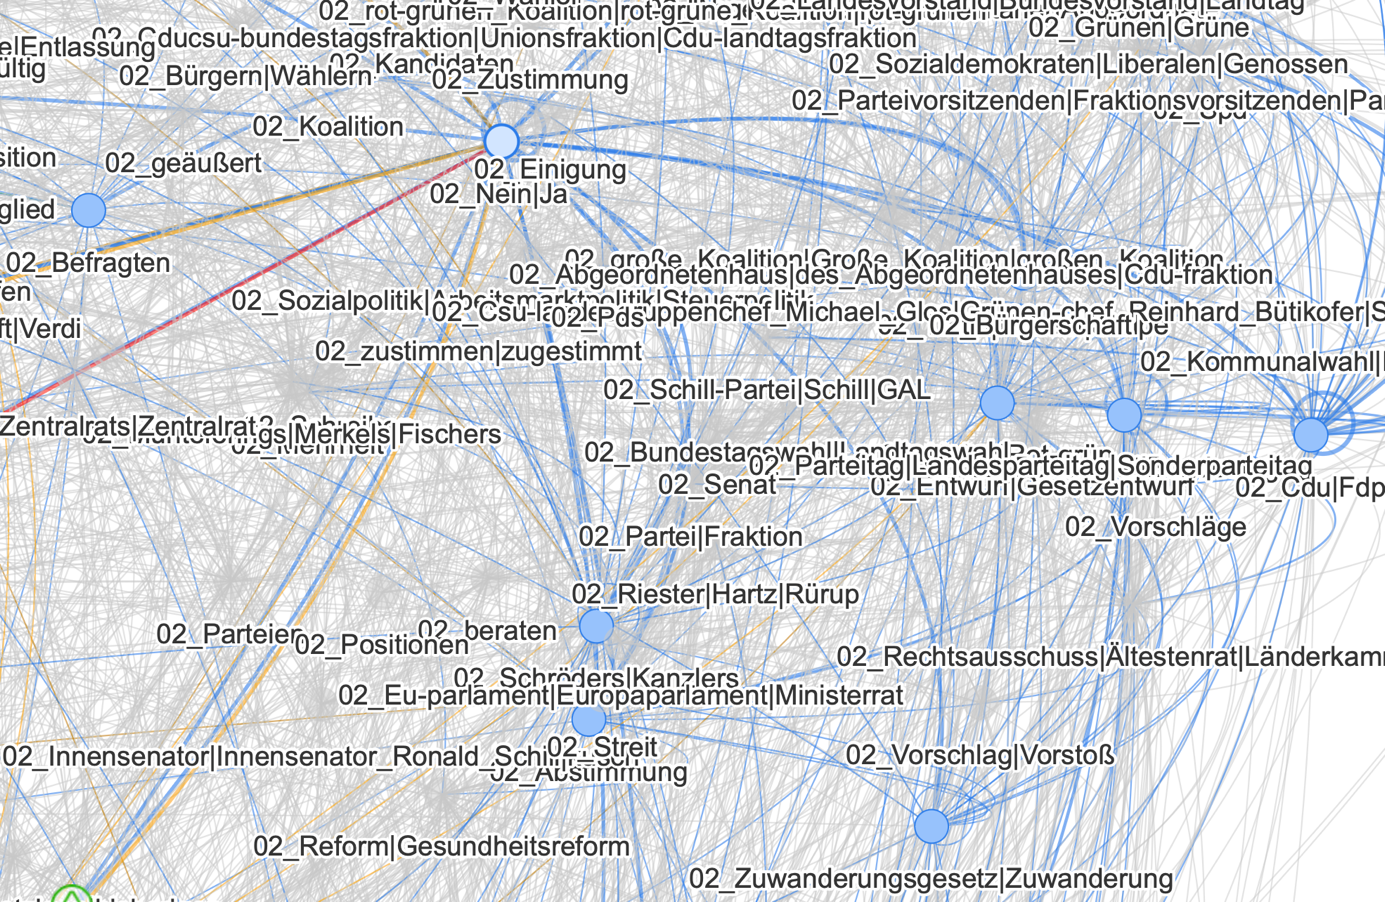
\includegraphics[width=\textwidth]{figures/media/image22.png}
  \caption{\label{fig:politik-beispiel}Ausschnitt aus dem thematischen Teil-Frame ‚Politik` am Beispiel des Clusters \cluster{02\_Nein{\breakbar}Ja}.}
\end{figure}

\largerpage[2]
Die Community ‚Politik` (\figref{fig:politik-beispiel}) umfasst (tages\mbox{-})politische Zusammenhänge. Die hier vertretenen Frame-Elemente umfassen insbesondere Akteure (z.\,B. \cluster{sp\_Afd{\breakbar}Npd}, \cluster{02\_Politiker{\breakbar}Kritiker}, \cluster{11\_Wähler}, \cluster{14\_Csu}) und Praktiken (z.\,B. \cluster{99\_Anhörung{\breakbar}Sondersitzung}, \cluster{02\_Wahl}, \cluster{14\_Debatte{\breakbar}Diskussion}) dieses Themenfeldes. Die Rolle der einzelnen FE im Extremismus-Frame kann dabei sehr unterschiedlich ausfallen. Akteure wie die NPD gelten selbst als extremistisch und sind einerseits wie alle politischen Parteien mit angeschlossenen FE wie \cluster{08\_Landtag}, \cluster{08\_Stimmen}, \cluster{08\_Parteitag} versehen. Die NPD weist aber auch eine starke Verankerung im Bereich der Demonstrationen (\cluster{08\_Demonstrationen{\breakbar}Kundgebung{\breakbar}Demo}, \cluster{08\_protestiert{\breakbar}demonstriert}) und mit anderen demonstrierenden Akteuren der rechten und linken Extreme (\cluster{08\_Autonomen{\breakbar}Antifas{\breakbar}Antifa}) sowie zu rechtsextremen Akteuren bzw. Attribuierungen (\cluster{08\_Rechtsextremisten{\breakbar}Neonazis{\breakbar}Rechtsextremen}, \cluster{08\_Fundamentalisten{\breakbar}rechtsradikalen{\breakbar}extremistische}) auf. Auch juristische Zusammenhänge wie \cluster{08\_Verbot} schlagen sich im Frame dieses Akteurs nieder. Andere politische Akteure wie \cluster{02\_Johannes\_Rau{\breakbar}Oskar\_Lafontaine{\breakbar}Helmut{\breakbar}Kohl} sind hingegen fast ausschließlich innerhalb der Community ‚Politik` vernetzt und werden nicht als extremistisch geframet. Es können außerdem politische Projekte bzw. Gesetzesänderungen in diesem Cluster verankert sein, so etwa das FE \cluster{02\_Agenda\_2010{\breakbar}Reformen{\breakbar}Hartz\_Iv}. Warum dieses vielleicht nicht ohne Weiteres für den Extremismusdiskurs einschlägige Cluster Teil des Frames ist, wird über die Betrachtung der angeschlossenen FE deutlich, die Aufschluss über das Framing der Reform geben. Vor allem die Vernetzung zum Bereich der Demonstrationen (\cluster{02\_Protest\_gegen{\breakbar}Protest}, \cluster{02\_Autonomen{\breakbar}Antifa{\breakbar}Rechtsextremisten}, \cluster{02\_Demonstrationen{\breakbar}Protestaktionen{\breakbar}Demos}, \cluster{02\_aufgerufen}) sowie den gesellschaftlichen Folgen der Gesetzesänderung (\cluster{02\_Zorn{\breakbar}Unmut{\breakbar}Wut}, \cluster{02\_Verwerfungen{\breakbar}Unsicherheiten{\breakbar}Unwägbarkeiten}) aufgrund des ausgeprägten außerparlamentarischen Protests gegen die Reform weist dabei Ähnlichkeiten zum Framing von Extremismus auf.

\begin{figure}[b]
  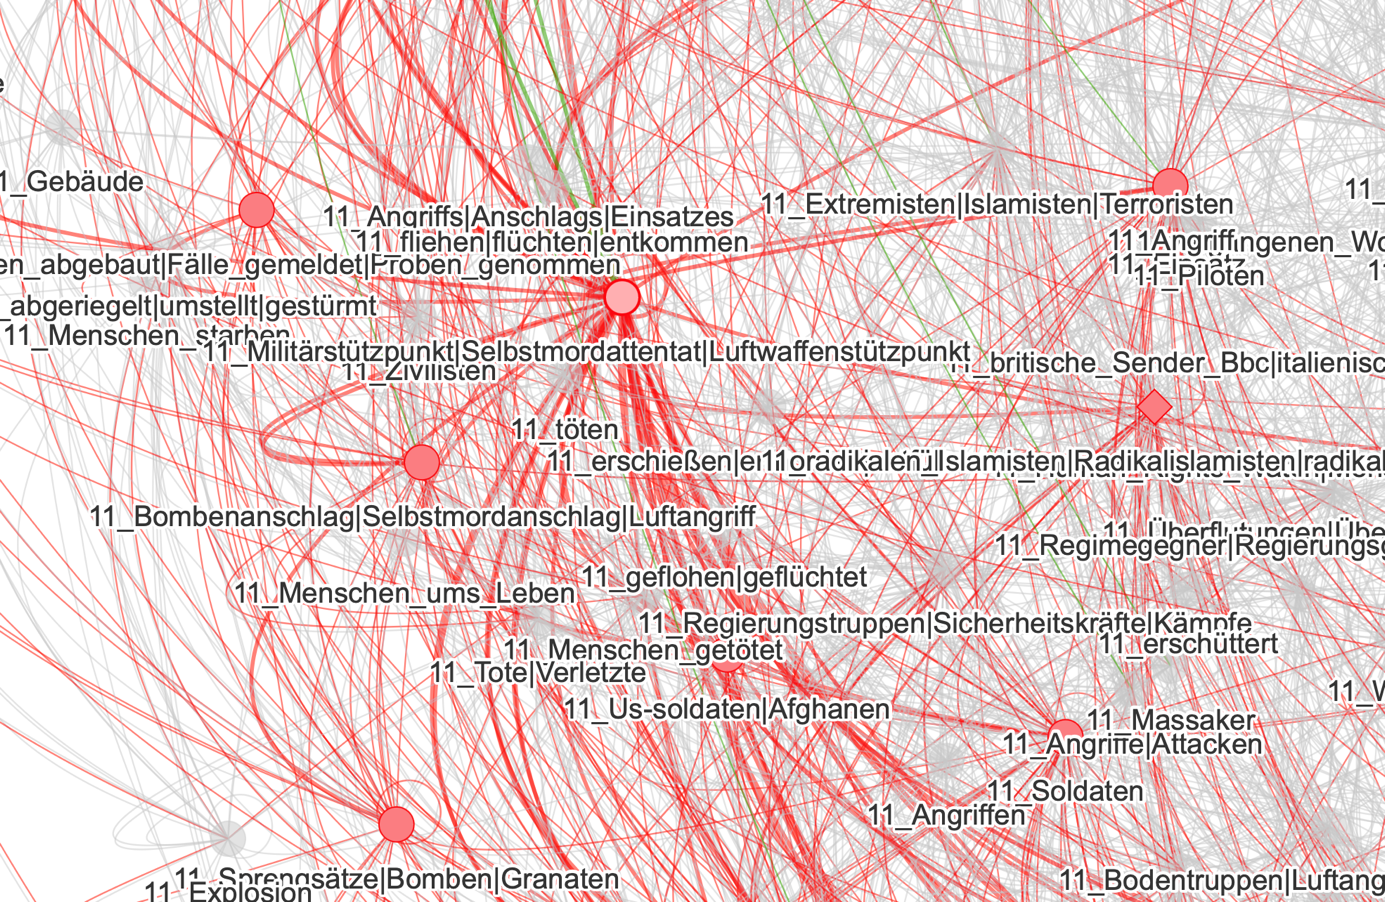
\includegraphics[width=\textwidth]{figures/media/image23.png}
  \caption{\label{fig:krieg-beispiel}Ausschnitt aus dem thematischen Teil-Frame ‚Krieg \& Islamismus` am Beispiel des Clusters \cluster{11\_Militärstützpunkt{\breakbar}Selbstmordattentat{\breakbar}Luftwaffenstützpunkt}.}
\end{figure}

Das Cluster ‚Krieg \& Islamismus` (\figref{fig:krieg-beispiel}) beinhaltet insbesondere kriegerische Handlungen (\cluster{02\_Tötung}, \cluster{14\_Luftschläge{\breakbar}Luftangriffe{\breakbar}Luftangriffen}, \cluster{we\_Angriffen}), Akteure (z.\,B. \cluster{02\_Iraker}, \cluster{11\_Regierungstruppen{\breakbar}Sicherheitskräfte{\breakbar}Kämpfe}, \cluster{14\_Bundeswehr}), Orte (z.\,B. \cluster{14\_Nordwesten\_Syriens{\breakbar}Nordosten\_Syriens{\breakbar}Norden\_Syriens}, \cluster{ta\_Gebiet}), Waffen und Kriegsgerät (z.\,B. \cluster{08\_Kampfjets{\breakbar}Kampfflugzeuge{\breakbar}Luftwaffe}, \cluster{we\_Handgranaten{\breakbar}Maschinengewehre{\breakbar}Pistolen}) sowie Attribute (z.\,B. \cluster{ta\_militärische{\breakbar}militärischen{\breakbar}militärischer}). Auch islamistische Handlungen (z.\,B. \cluster{14\_Anschläge{\breakbar}Terroranschläge{\breakbar}Attentate}, \cluster{14\_Attentäter{\breakbar}Selbstmordattentäter}) und Akteure (z.\,B. \cluster{08\_Extremisten{\breakbar}Taliban{\breakbar}Islamisten, 14\_IS\_Miliz{\breakbar}Terrormiliz{\breakbar}Isis}) fallen in dieses Netzwerk-Cluster.

\begin{figure}[t]
  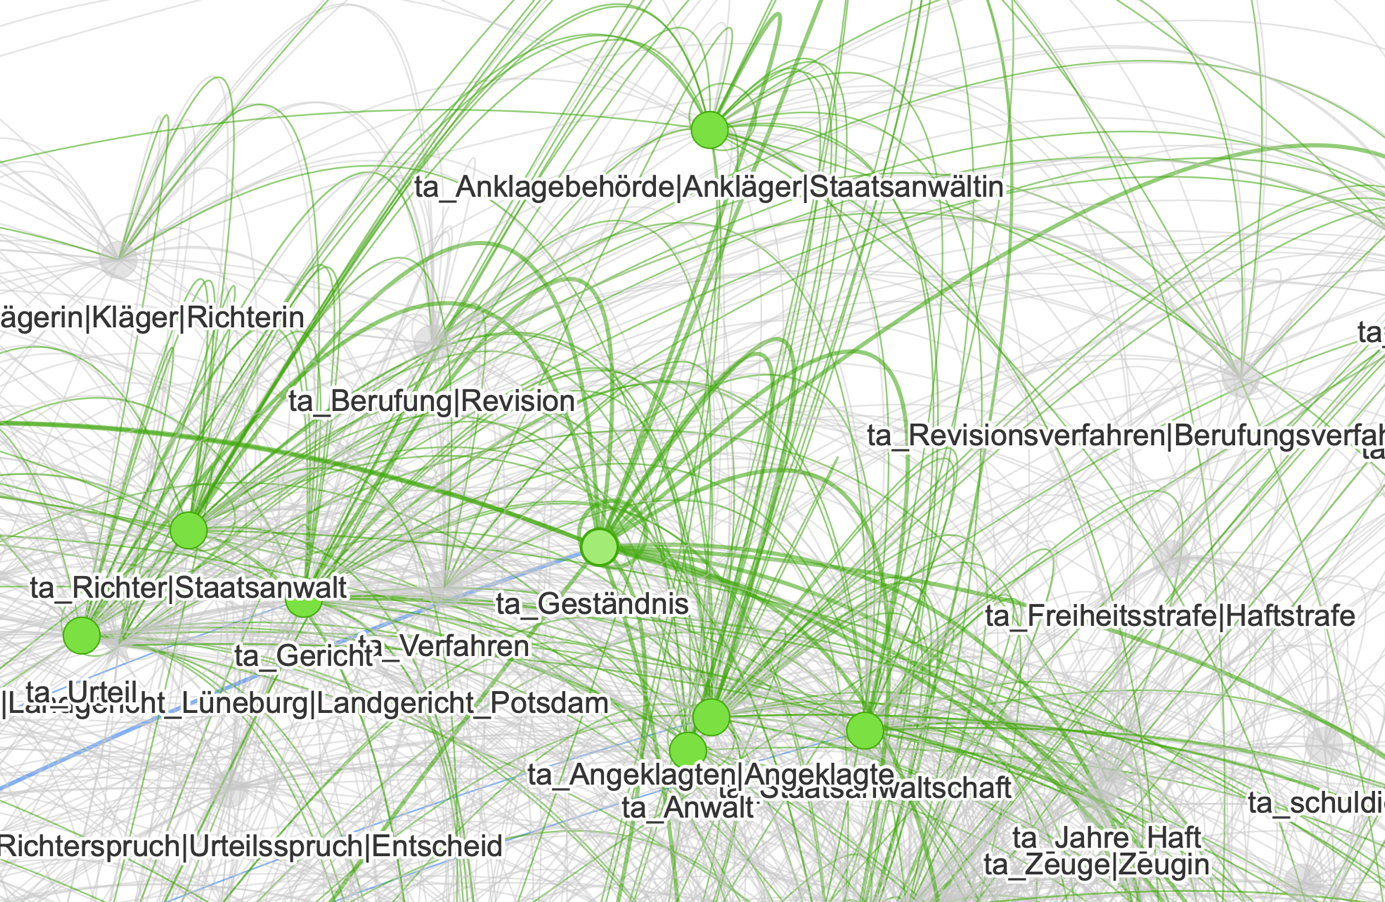
\includegraphics[width=\textwidth]{figures/media/image24.png}
  \caption{\label{fig:straftaten-beispiel}Ausschnitt aus dem thematischen Teil-Frame ‚Straftaten \& Juristisches` am Beispiel des Clusters \cluster{ta\_Geständnis}.}
\end{figure}

Im thematischen Teil-Frame ‚Straftaten \& Juristisches` (\figref{fig:straftaten-beispiel}) finden sich u.\,a. einzelne Straftaten (z.\,B. \cluster{05\_Gewalttaten{\breakbar}Straftaten{\breakbar}Morde}, \cluster{14\_Verbrechen}, \cluster{14\_Diebstähle{\breakbar}Körperverletzungen{\breakbar}Sachbeschädigungen}, \cluster{sp\_Sexualstraftaten{\breakbar}Körperverletzungen{\breakbar}Sexualdelikte}), gerichtliche und institutionelle Akteure der Strafverfolgung bzw. Ermittlungsbehörden (\cluster{02\_Staatsanwaltschaft}, \cluster{14\_Gerichtshof{\breakbar}Bundesgericht{\breakbar}Berufungsgericht}, \cluster{14\_Verteidiger{\breakbar}Verteidigung}, \cluster{14\_NSA{\breakbar}Bnd, sp\_schuldig\_gesprochen{\breakbar}zum\_Tode\_verurteilt{\breakbar}freigesprochen}) und einzelne Angeklagte (\cluster{08\_Ankläger{\breakbar}Kachelmann{\breakbar}Staatsanwältin}, \cluster{14\_Beate\_Zschäpe{\breakbar}Zschäpe{\breakbar}Nsu-prozess}, \cluster{we\_Mollath{\breakbar}seinen\_Mandanten{\breakbar}Gäfgen}).

Eine weitere in allen Subkorpora emergierende Netzwerk-Community (\figref{fig:staat-beispiel}) ist thematisch etwas vager, aber insofern äußerst relevant für den Extremismusdiskurs, als sie die FdGO, also die definitorische Antithese zum Extremismus, widerspiegelt.

\begin{figure}
  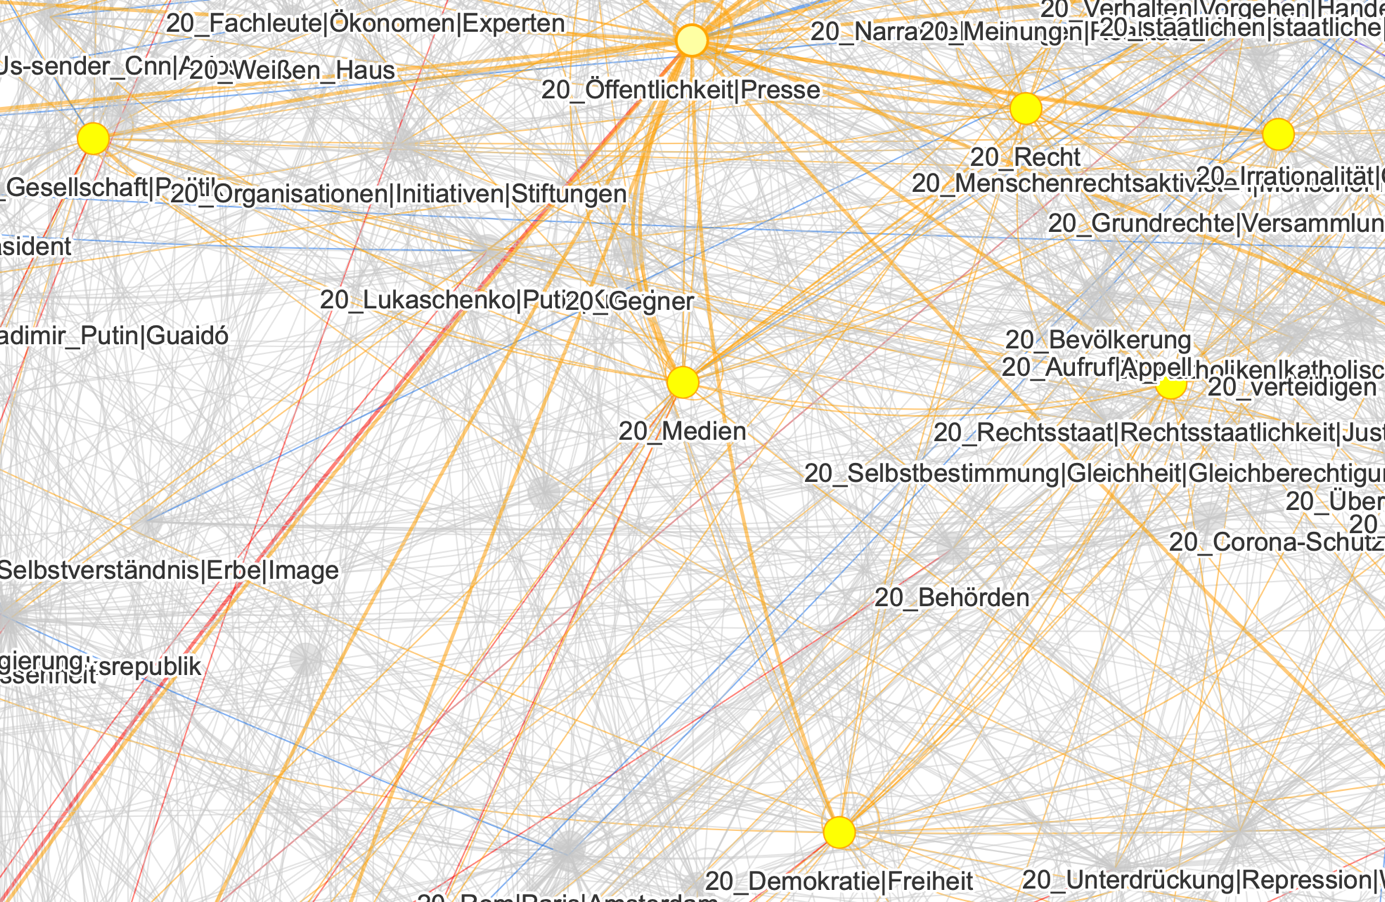
\includegraphics[width=\textwidth]{figures/media/image25.png}
  \caption{\label{fig:staat-beispiel}Ausschnitt aus dem thematischen Teil-Frame ‚Staat, FdGO \& Gesellschaft` am Beispiel des Clusters \cluster{20\_Öffentlichkeit{\breakbar}Presse}.}
\end{figure}

Hier sind FE gebündelt, die Grundrechte (\cluster{99\_Grundreche{\breakbar}Meinungsfreiheit{\breakbar}Menschenwürde}, \cluster{08\_Schutz}, \cluster{14\_Chancengleichheit{\breakbar}Selbstbestimmung{\breakbar}Gleichberechtigung}, \cluster{14\_Menschenwürde{\breakbar}Religionsfreiheit{\breakbar}Freiheitsrechte}), einzelne Werte (\cluster{05\_Ehre}, \cluster{14\_Solidarität}, \cluster{14\_Ideale{\breakbar}Ideologie{\breakbar}Überzeugungen}, \cluster{ta\_Toleranz}), die Organisation von Staat und Gesellschaft (\cluster{11\_Republik}, \cluster{14\_Gesellschaft}, \cluster{14\_Bundesrepublik}, \cluster{ta\_Staates}), gesellschaftliche Gruppen (\cluster{02\_Bürger}, \cluster{14\_Lesben{\breakbar}Schwule{\breakbar}Schwulen}, \cluster{14\_Elite{\breakbar}Eliten{\breakbar}Mittelschicht}, \cluster{14\_Religion} ), aber auch Aushandlungsprozesse und Bedrohungen ebendieser Ordnung (\cluster{02\_Kampf\_gegen}, \cluster{14\_Debatte{\breakbar}Diskussion}, \cluster{14\_verteidigen}, \cluster{14\_diskreditieren{\breakbar}provozieren{\breakbar}instrumentalisieren}, \cluster{20\_bedroht{\breakbar}gefährdet}, \cluster{20\_Antisemitismus{\breakbar}Rassismus{\breakbar}Rechtsextremismus}) widerspiegeln. Auch einschneidende negative historische Ereignisse bzw. Gräueltaten sind in diesem Cluster häufig enthalten (\cluster{14\_Barbarei{\breakbar}Grausamkeit{\breakbar}Brutalität}, \cluster{14\_Zweiten\_Weltkrieg{\breakbar}Ersten\_Weltkrieg}, \cluster{14\_Völkermord{\breakbar}Genozid{\breakbar}Armenien}). Dass diese besonders schweren historischen Verbrechen regelmäßig in diesem Netzwerk-Cluster enthalten sind, macht einen deutlichen Unterschied im Framing im Vergleich zu den zeitgenössischen Kriegen deutlich: Sie werden medial nicht in erster Linie als kriegerische Handlungen thematisiert, bei denen an bestimmten Orten mithilfe einzelner Waffen Angriffe verübt wurden, sondern insbesondere in ihrer historisch-gesellschaftlichen Bedeutung.

\begin{figure}
  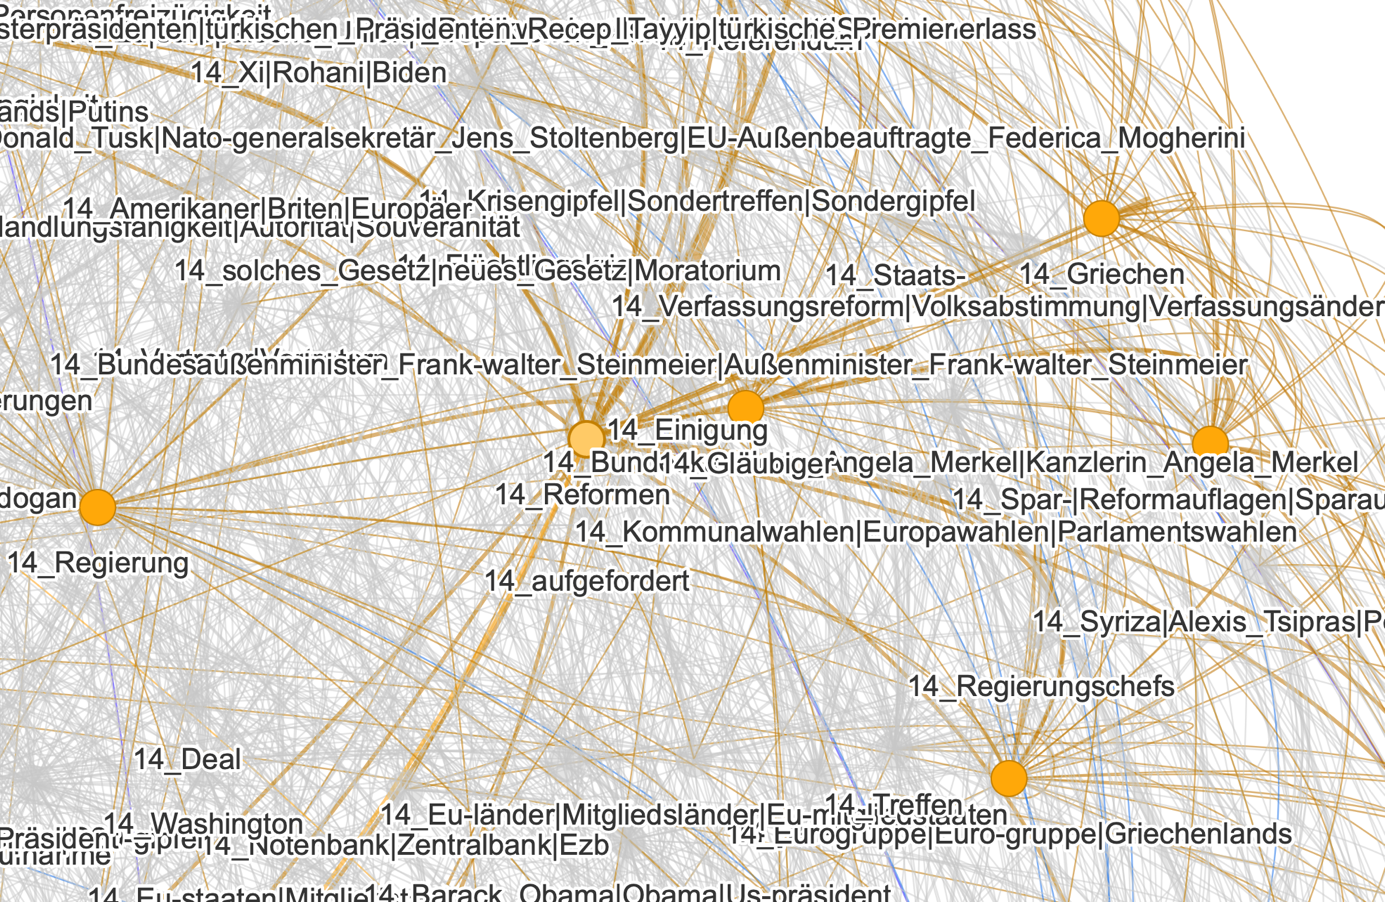
\includegraphics[width=\textwidth]{figures/media/image26.png}
  \caption{\label{fig:aussenpolitik-beispiel}Ausschnitt aus dem thematischen Teil-Frame ‚Außenpolitik` am Beispiel des Clusters \cluster{14\_Reformen}.}
\end{figure}

\begin{figure}
  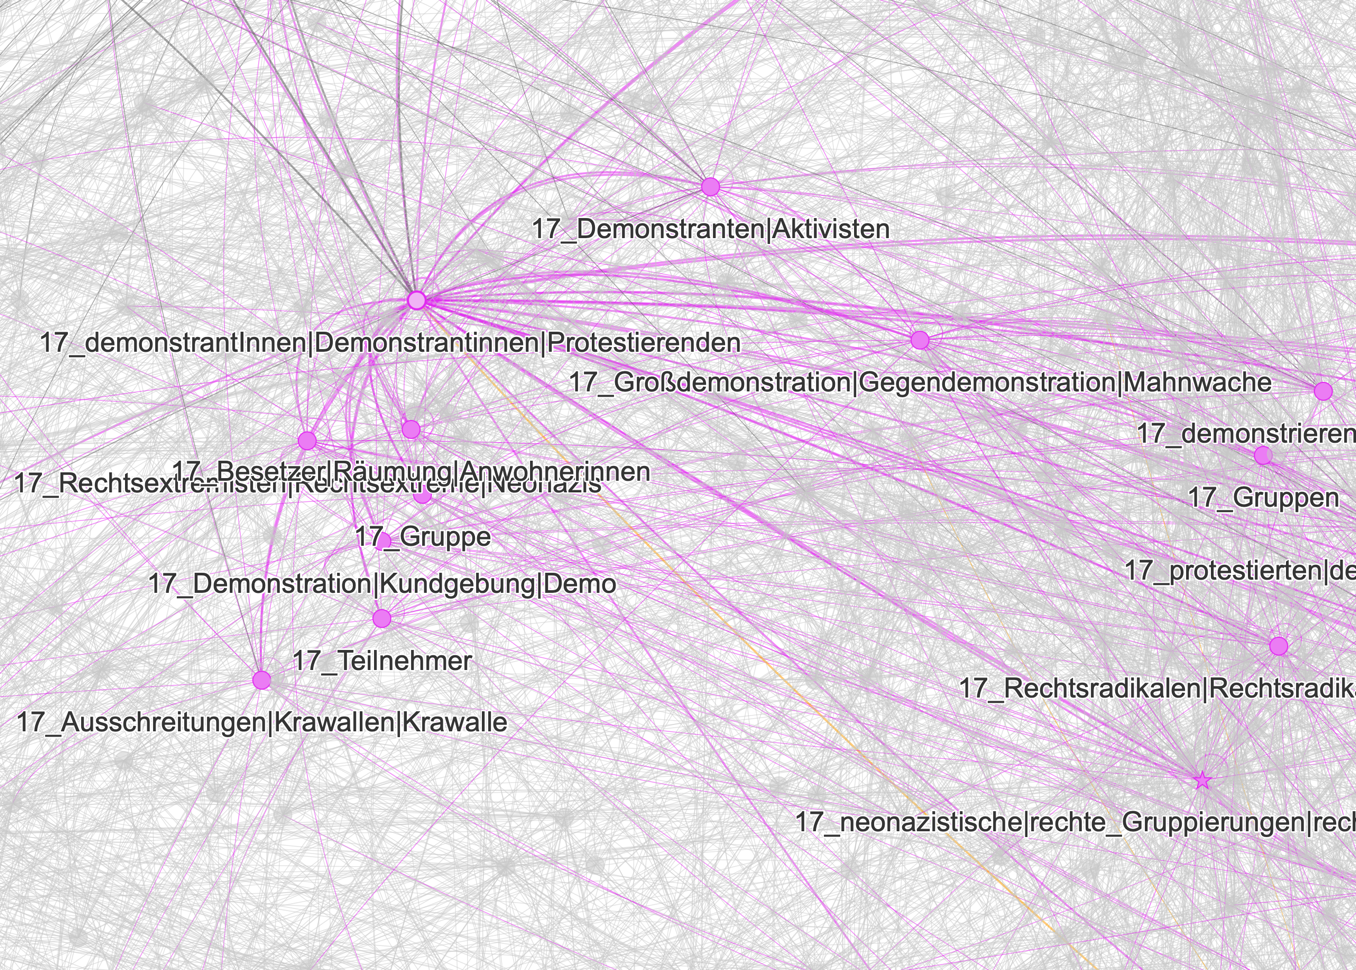
\includegraphics[width=\textwidth]{figures/media/image27.png}
  \caption{\label{fig:demonstrationen-beispiel}Ausschnitt aus dem thematischen Teil-Frame ‚Demonstrationen \& politischer Extremismus` am Beispiel des Clusters 17\cluster{\_demonstrantInnen{\breakbar}Demonstrantinnen{\breakbar}Protestierenden}.}
\end{figure}

Neben diesen vier in jedem Teilkorpus zu Tage tretenden Communities finden sich zwei weitere Cluster, die zwar nicht in allen, aber in den meisten der Subkorpora identifiziert wurden. So tritt die Community ‚Außenpolitik` (\figref{fig:aussenpolitik-beispiel}) in den Subkorpora 2002--2004, 2005--2007, 2008--2010, 2011--2013, 2014--2016 und \textsc{Spiegel} auf und die Community ‚Demonstrationen \& politischer Extremismus` in den Subkorpora 2002--2004, 2005--2007, 2008--2010, 2014--2016, 2017--2019, \textsc{Taz} und \textsc{Welt}. Im Cluster Außenpolitik finden sich internationale Akteure und Orte (\cluster{05\_Uno{\breakbar}Vereinten\_Nationen{\breakbar}UN}, \cluster{05\_Entwicklungsländer{\breakbar}Industriestaaten{\breakbar}Industrieländer}, \cluster{05\_Außenminister{\breakbar}Regierungschefs{\breakbar}Botschafter}, \cluster{05\_Europa{\breakbar}Deutschland{\breakbar}Amerika}, \cluster{11\_Notenbank{\breakbar}Zentralbank{\breakbar}Bundesbank,} \cluster{sp\_Burma{\breakbar}Myanmar{\breakbar}Simbabwe}), Praktiken (\cluster{05\_Gipfels{\breakbar}Treffens{\breakbar}G-8-Gipfels}, \cluster{05\_Scheitern}, \cluster{05\_Versprechen, 11\_Notkredite{\breakbar}Hilfskredite{\breakbar}Rettungsfonds}) sowie außenpolitische und diplomatische Projekte (\cluster{05\_Beitritt{\breakbar}Eu-beitritt}, \cluster{14\_Reformen}). Die Community ‚Demonstrationen \& politischer Extremismus` (\figref{fig:demonstrationen-beispiel}) umfasst Akteure, die an Demonstrationen teilnehmen (\cluster{05\_Gewerkschaften, 17\_Demonstranten{\breakbar}Aktivisten}), Akteure des Rechts- und Linksextremismus (\cluster{17\_Rechtsextremisten{\breakbar}Rechtsextreme{\breakbar}Neonazis}, \cluster{17\_Besetzer{\breakbar}Räumung{\breakbar}Anwohnerinnen}, \cluster{ta\_Antifas{\breakbar}Skins{\breakbar}Antifaschisten}) sowie Attribuierungen zu Demonstrationen (\cluster{ta\_friedlich}, \cluster{ta\_Ausschreitungen{\breakbar}Krawalle{\breakbar}Krawallen}, \cluster{we\_gewalttätigen\_Auseinandersetzungen{\breakbar}Straßenschlachten{\breakbar}gewaltsamen\_Auseinandersetzungen}).

\begin{figure}
  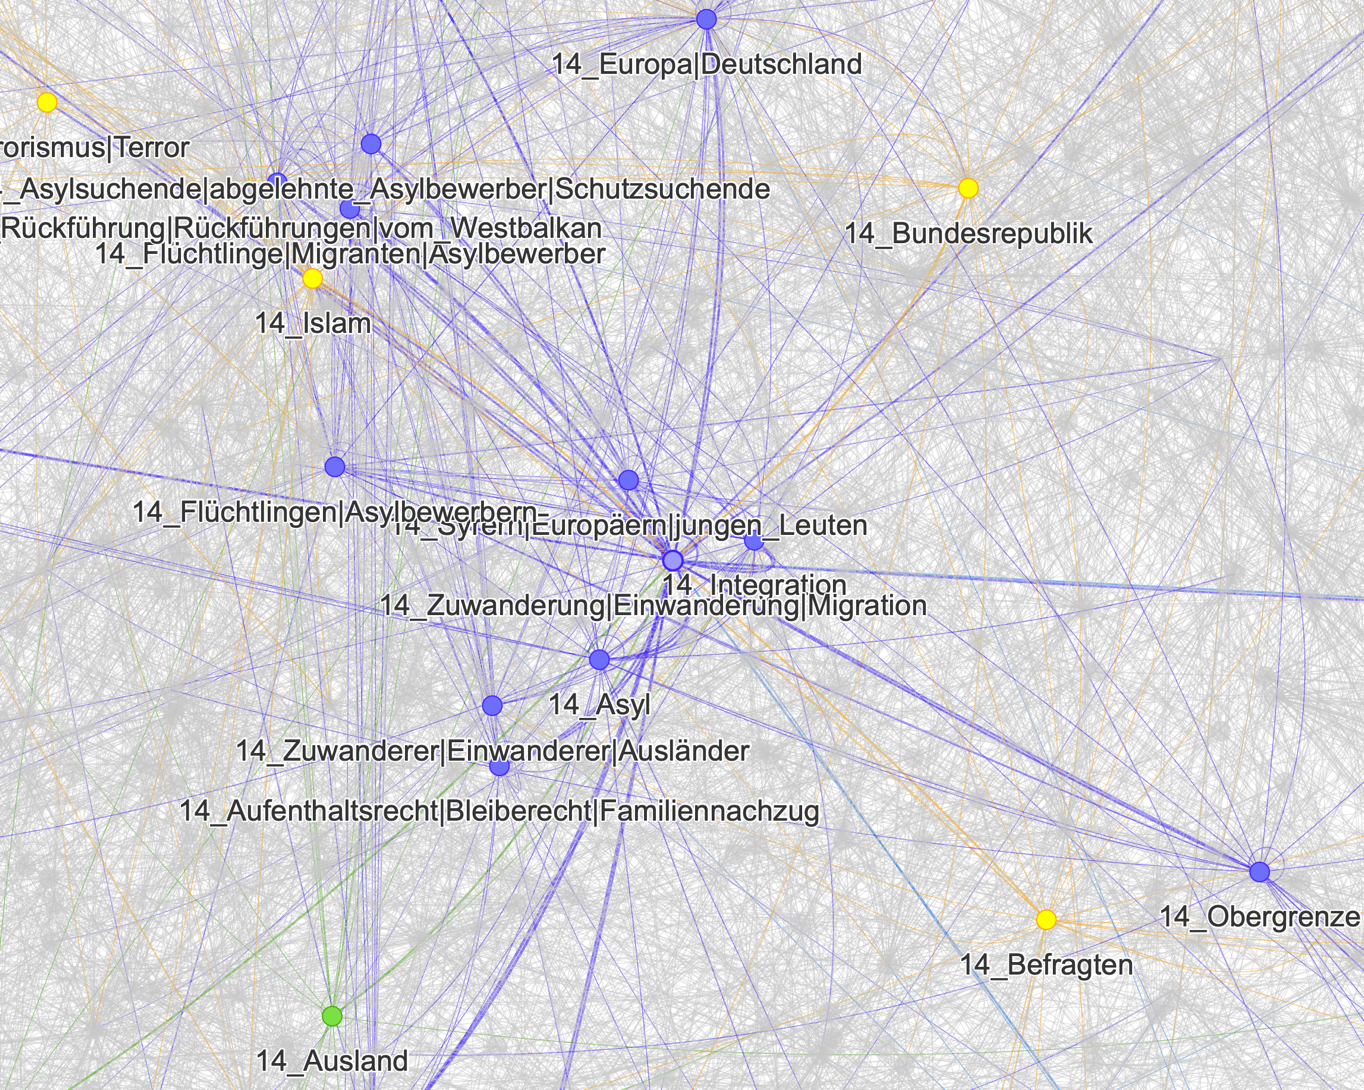
\includegraphics[width=\textwidth]{figures/media/image28.png}
  \caption{\label{fig:flucht-beispiel}Ausschnitt aus dem thematischen Teil-Frame ‚Flucht \& Migration` am Beispiel des Clusters 14\cluster{\_Zuwanderung{\breakbar}Einwanderung{\breakbar}Migration}.}
\end{figure}

Letztlich finden sich einige weitere Cluster, die nur in einzelnen Teilkorpora oder auch nur einmalig identifiziert werden. Dies betrifft das Cluster ‚Migration \& Flucht` (\figref{fig:flucht-beispiel}) in den Subkorpora 2014--2016, 2017--2019, \textsc{Taz} und \textsc{Welt} (\cluster{we\_Asylverfahren{\breakbar}Asylanträge}, \cluster{14\_Zuwanderer{\breakbar}Einwanderer{\breakbar}Ausländer}), ‚Geheimdienste` im \textsc{Welt}-Teilkorpus (\cluster{we\_Bnd{\breakbar}NSA}, \cluster{we\_Telefonaten{\breakbar}Anrufen{\breakbar}Kontakten}), ‚Unglücke, Attentate \& Gedenken` in den Subkorpora 2014--2016, 2017--2019, 2020--2021 und \textsc{Spiegel} (\cluster{14\_Lastwagen{\breakbar}LKW}, \cluster{17\_Attentäter}, \cluster{20\_Hanau}, \cluster{sp\_Unglück}), ‚Religion` im \textsc{Taz}-Subkorpus (\cluster{ta\_Gemeinschaft}, \cluster{ta\_Gläubige{\breakbar}Gläubigen{\breakbar}Pilger}) sowie ‚Nationalsozialismus \& DDR` im \textsc{Spiegel}-Teilkorpus (\cluster{sp\_Ddr}, \cluster{sp\_Nationalsozialisten{\breakbar}Nazis{\breakbar}Nationalsozialismus}). In zwei Fällen wurden auch Communities algorithmisch identifiziert, die jeweils nur ein Cluster umfassen (\cluster{99\_Anhänger{\breakbar}Gegner} und \cluster{02\_Erklärung}) und daher nicht weiter berücksichtigt wurden.

\section{Mesostruktur: Extremismusvarianten-Frames}\label{mesostruktur-extremismusvarianten-frames}

\subsection{Der Zeitraum 1999--2001}\label{der-zeitraum-1999-2001}

\subsubsection{\texorpdfstring{\emph{Corpus-driven} Voranalyse: Cluster mit hoher Cosinus-Distanz im Vergleich zum Gesamtkorpus}{Corpus-driven Voranalyse: Cluster mit hoher Cosinus-Distanz im Vergleich zum Gesamtkorpus}}\label{corpus-driven-voranalyse-cluster-mit-hoher-cosinus-distanz-im-vergleich-zum-gesamtkorpus}

Da der Zeitraum 1999--2001 das in diachroner Perspektive erste Teilkorpus darstellt, können an dieser Stelle keine semantischen Äquivalenzen von Clustern oder Verschiebungen im Vergleich zu einem vorhergehenden Zeitraum berichtet werden (siehe zu den quantitativen Voranalysen \chapref{vorgehen-und-zielsetzung}). Behelfsweise werden daher die Cluster-Distanzen zum auf dem Gesamtkorpus trainierten Word-Embedding-Modell (dem \emph{compass}) berechnet. Die Top 20 so ermittelten Cluster sind in \tabref{tab:cluster-high-cosine-distance-1999} dargestellt. Es zeichnen sich in der Liste der Cluster insbesondere im Bereich der Außenpolitik wesentliche Veränderungen ab. Cluster wie \cluster{99\_Al\_Gore{\breakbar}Gore{\breakbar}George\_W\_Bush} und \cluster{99\_Vizepräsident\_Al\_Gore{\breakbar}Mccain{\breakbar}John\_Mccain} weisen zum einen auf die US-amerikanische Präsidentschaftswahl des Jahres 2000 hin, zum anderen mit \cluster{99\_Irak} auch auf die im Anschluss an 9/11 geführten Debatten um die Rolle des Iraks bei den Anschlägen. Auch der Nahostkonflikt (\cluster{99\_Gaza-streifen{\breakbar}Westjordanland{\breakbar}Gazastreifen, 99\_ Ehud\_Barak{\breakbar}Ariel\_Scharon{\breakbar}Jassir\_Arafat}), außerparlamentarischer Protest (\cluster{99\_Neckarwestheim{\breakbar}Philippsburg{\breakbar}Atomtransporte}), kontroverse politisch-gesellschaftliche Debatten (\cluster{99\_Homo-ehe{\breakbar}Unterschriftensammlung{\breakbar}doppelte\_Staatsbürgerschaft}) sowie die CDU-Spendengeldaffäre \cluster{(99\_Weyrauch{\breakbar}Walther\_Leisler\_Kiep{\breakbar}Horst\_Weyrauch)} klingen an.

\begin{table}[t]\small
\caption{Cluster mit hoher Cosinus-Distanz im Vergleich zum Gesamtkorpus.}
\label{tab:cluster-high-cosine-distance-1999}
\begin{tabularx}{\textwidth}{X r}
\lsptoprule
Cluster & Cos.-Dist. \\
\midrule
\cluster{Al\_Gore{\breakbar}Gore{\breakbar}George\_W\_Bush} & 0.28 \\
\cluster{Spd-generalsekretär\_Franz\_Müntefering{\breakbar}Struck{\breakbar}CDU-Generalsekretärin\_Angela\_Merkel} & 0.26 \\
\cluster{Rühe{\breakbar}Möllemann{\breakbar}Wolfgang\_Schäuble} & 0.25 \\
\cluster{Vizepräsident\_Al\_Gore{\breakbar}Mccain{\breakbar}John\_Mccain} & 0.25 \\
\cluster{Neckarwestheim{\breakbar}Philippsburg{\breakbar}Atomtransporte} & 0.24 \\
\cluster{Weyrauch{\breakbar}Walther\_Leisler\_Kiep{\breakbar}Horst\_Weyrauch} & 0.24 \\
\cluster{Afp{\breakbar}ap{\breakbar}rtr} & 0.24 \\
\cluster{Ausnahmeregelung{\breakbar}Gesetzesänderung{\breakbar}Sonderregelung} & 0.24 \\
\cluster{rebellieren{\breakbar}ankämpfen{\breakbar}Parteiengesetz\_verstoßen} & 0.24 \\
\cluster{Irak} & 0.23 \\
\cluster{Ehud\_Barak{\breakbar}Ariel\_Scharon{\breakbar}Jassir\_Arafat} & 0.23 \\
\cluster{Jospin{\breakbar}Blair{\breakbar}Tony\_Blair} & 0.23 \\
\cluster{rot-grüne\_Koalition{\breakbar}Rot-grün{\breakbar}rot-grüne\_Regierung} & 0.22 \\
\cluster{Gipfel{\breakbar}Gipfeltreffen{\breakbar}Eu-gipfel} & 0.22 \\
\cluster{Verbrecher{\breakbar}Drogenhändler{\breakbar}Mafiosi} & 0.22 \\
\cluster{Oberlandesgericht{\breakbar}Olg{\breakbar}Bundesgerichtshof\_Bgh} & 0.22 \\
\cluster{Gaza-streifen{\breakbar}Westjordanland{\breakbar}Gazastreifen} & 0.22 \\
\cluster{Homo-ehe{\breakbar}Unterschriftensammlung{\breakbar}doppelte\_Staatsbürgerschaft} & 0.21 \\
\cluster{Kurden} & 0.21 \\
\cluster{europäischen\_Union\_Eu{\breakbar}europäische\_Union{\breakbar}Wto} & 0.21 \\
\lspbottomrule
\end{tabularx}
\end{table}

\subsubsection{Rechts- und Linksextremismus}\label{rechts--und-linksextremismus}

Es lassen sich in diesem Teilkorpus insbesondere die folgenden Cluster ausmachen, die auf Basis von Diskurswissen mit recht großer Sicherheit als Bestandteile eines Rechtsextremismus-Frames zu lesen sind: \cluster{99\_Neonazis{\breakbar}Skinheads{\breakbar}Rechtsextremisten (rechtsextreme Akteure und Akteure bei Demonstrationen)}, \cluster{99\_NPD}, \cluster{99\_Nazis}, \cluster{99\_Holocaust{\breakbar}Nationalsozialismus}, \cluster{99\_Fremdenfeindlichkeit{\breakbar}Ausländerfeindlichkeit{\breakbar}Rassismus (Charakteristika des Rechtsextremismus)}. Ein Problem für korpuslinguistische Verfahren, die auf Types beruhen, stellen homonyme oder polyseme Wörter dar (siehe \chapref{moegliche-fallstricke-bei-der-interpretation}). Dies betrifft in diesem Zeitraum das Cluster \cluster{99\_Republikaner{\breakbar}Demokraten}, dessen Wörter sich gut in einem Cluster zusammenfassen lassen, wenn sie auf die beiden US-amerikanischen Parteien referieren. Zugleich sind die Republikaner jedoch auch eine Partei des äußeren rechten Spektrums in Deutschland. Dieser Unterschied wird bei der Berechnung der Word Embeddings bzw. Cluster sowie der Kollokationen ebendieser nicht berücksichtigt. Mithin fließen beide Bedeutungen in die Positionierung des Clusters im Graphen ein und es weist einerseits Verbindungen zu Clustern wie \cluster{99\_Senat} oder \cluster{99\_Clinton{\breakbar}Bush{\breakbar}Putin} auf, andererseits auch zu \cluster{99\_Npd} und \cluster{99\_Kommunalwahlen{\breakbar}Europawahl{\breakbar}Europawahlen}.

Wählt man alle identifizierten Cluster im Graphen aus, lässt sich der Recht\-sextremismus-Frame dieses Zeitraumes (siehe \figref{fig:rechtsextremismus-frame-1999-2001} in \chapref{kollokation-von-word-embedding-clustern-als-frame-relationen-und-perspektivierung-kollokationsnetzwerke-als-frames}) visualisieren und die jeweilige Perspektivierungsleistung der einzelnen FE erschließen, indem die angeschlossenen FE -- unter Berücksichtigung ihrer Verortung in den thematischen Teil-Frames -- betrachtet werden. An den Akteur-Clustern \cluster{99\_Neonazis{\breakbar}Skinheads{\breakbar}Rechtsextremisten}, \cluster{99\_NPD} und \cluster{99\_Nazis} wird -- wie in \chapref{kollokation-von-word-embedding-clustern-als-frame-relationen-und-perspektivierung-kollokationsnetzwerke-als-frames} bereits umrissen -- deutlich, dass sie zwar alle Akteure des Rechtsextremismus enthalten, jedoch deutlich unterschiedliche Perspektivierungsleistungen erbringen.

\begin{figure}[t]
  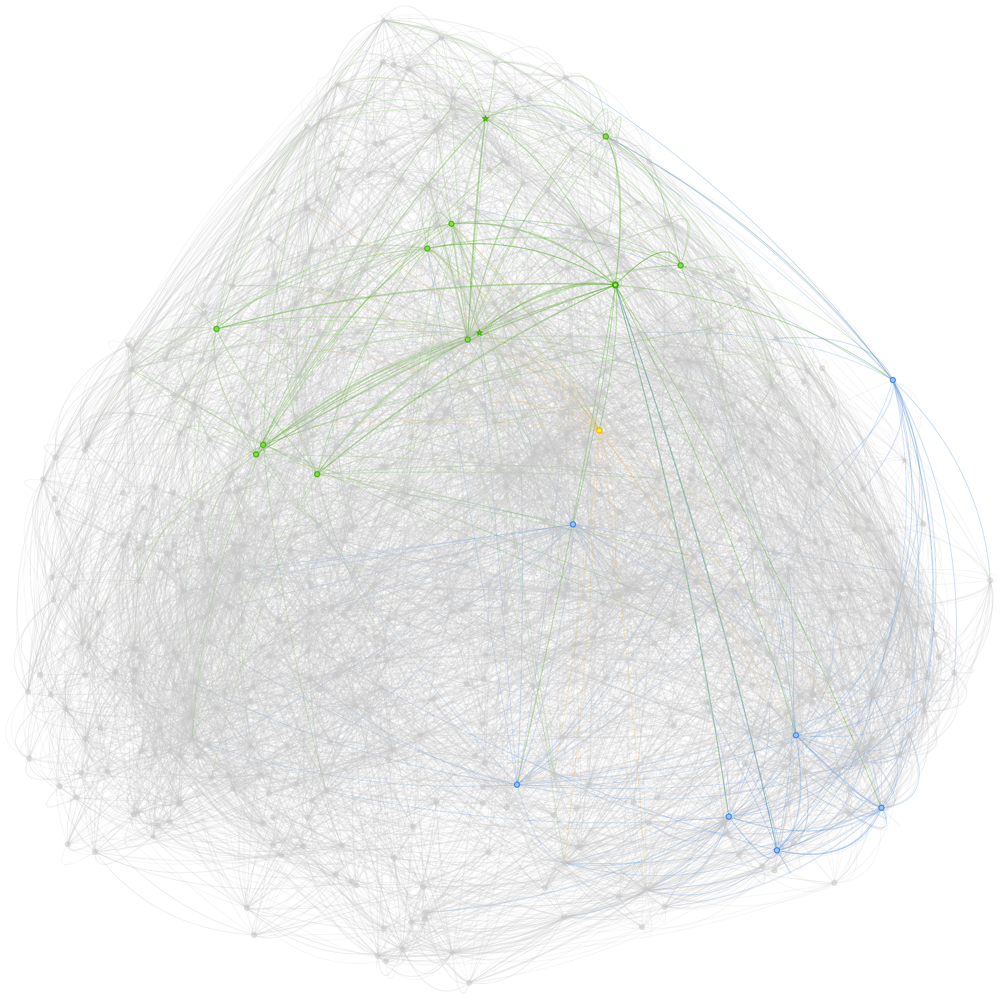
\includegraphics[width=.8\textwidth]{figures/media/image29.png}
  \caption{\label{fig:npd-frame}Thematische Verankerung des NPD-Frames.}
\end{figure}

So sind an das NPD-FE, das im juristischen Netzwerk-Cluster liegt, fast ausschließlich FE aus den Bereichen ‚Politik` und ‚Straftaten \& Juristisches` angeschlossen (siehe \figref{fig:npd-frame}). Durch den Anschluss an ersteren Bereich und FE wie \cluster{99\_Mitglieder}, \cluster{99\_Partei}, \cluster{99\_Antrag} wird die NPD als politische Partei geframet. Die Vernetzung in zweiterem Bereich macht hingegen den Status der NPD als rechtsextreme Partei deutlich. Zum einen finden sich hier die Cluster \cluster{99\_Verbot} und \cluster{99\_Bundesgerichtshof{\breakbar}Bgh{\breakbar}Bundesverfassungsgericht}, die das in diesem Zeitraum beginnende erste NPD-Verbotsverfahren zum Teil des verstehensrelevanten Wissens zum NPD- bzw. Rechtsextremismus-Frame machen; zum anderen Cluster wie \cluster{99\_Bnd{\breakbar}Fbi{\breakbar}Bka (Geheimdienste)}, \cluster{99\_Neonazis{\breakbar}Skinheads{\breakbar}Rechtsextremisten (rechtsextreme Akteure und Akteure bei Demonstrationen)}, \cluster{99\_Demonstrationen{\breakbar}Proteste{\breakbar}Protesten} oder \cluster{99\_Autonomen{\breakbar}Rechtsextremen{\breakbar}Aufmärsche (Demonstrationen des politischen Extremismus inkl. Akteuren, Demonstrationsformen, Charakteristika)}, die die Organisation von bzw. Beteiligung an Demonstrationen, Verflechtungen mit rechtsextremistischen Gruppen oder die Beobachtung durch den Verfassungsschutz abbilden.

\begin{figure}
  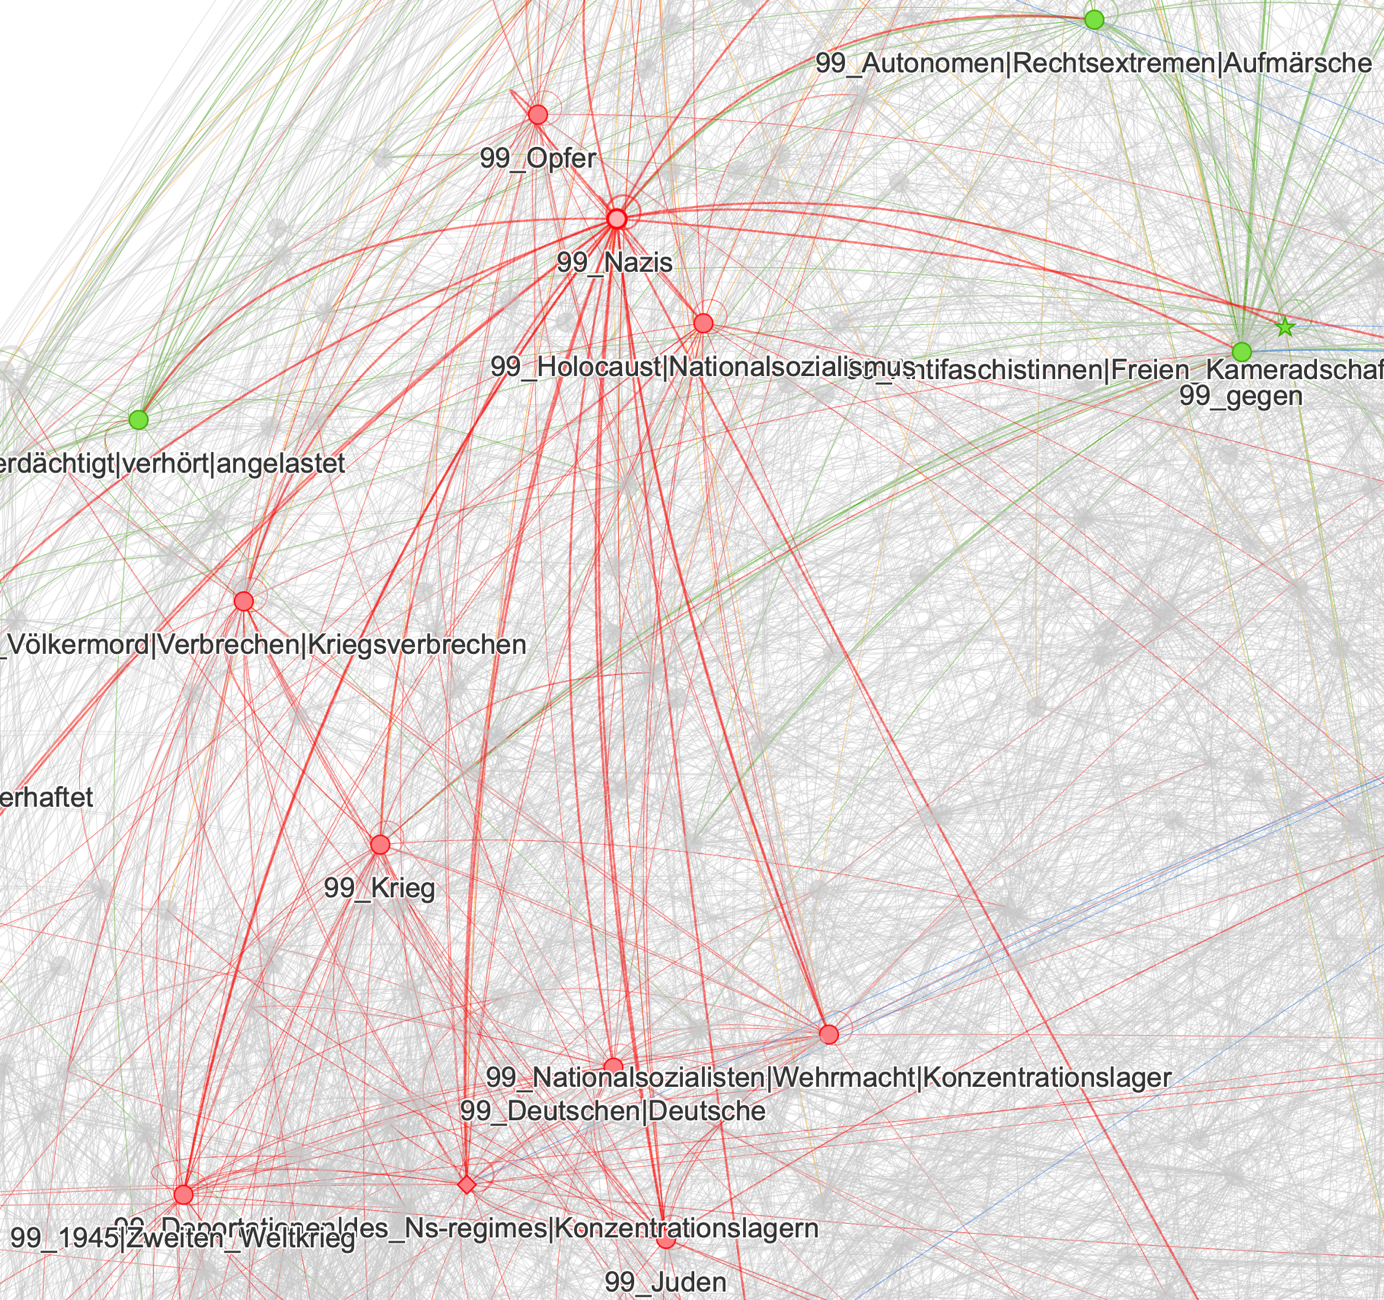
\includegraphics[width=\textwidth]{figures/media/image30.png}
  \caption{\label{fig:perspektivierung-nazis}Perspektivierung rechtsextremistischer Akteure durch das FE \cluster{99\_Nazis}.}
\end{figure}

Das Cluster \cluster{99\_Nazi} hingegen prägt deutlich andere Verbindungen im Frame aus (siehe \figref{fig:perspektivierung-nazis}). Es gehört zum thematischen Teil-Frame ‚Krieg \& Islamismus` und ist in diesem auch am meisten vernetzt, wobei fast alle hier angeschlossenen FE einen Bezug zur Zeit des Zweiten Weltkriegs aufweisen (u.\,a. \cluster{99\_Juden}, \cluster{99\_Krieg}, \cluster{99\_1945{\breakbar}Zweiten\_Weltkrieg}, \cluster{99\_Völkermord{\breakbar}Verbrechen{\breakbar}Kriegsverbrechen}). Es weist jedoch auch einzelne Verbindungen in die Cluster ‚Staat, FdGO \& Gesellschaft` (u.\,a. \cluster{99\_Fremdenfeindlichkeit{\breakbar}Ausländerfeindlichkeit{\breakbar}Rassismus}) und ‚Straftaten \& Jurstisches` (\cluster{99\_Autonomen{\breakbar}Rechtsextremen{\breakbar}Aufmärsche}) auf, die zeigen, dass der Ausdruck \emph{Nazis} mitunter auch in Zusammenhang mit zeitgenössischen Phänomenen des Rechtsextremismus genutzt wird, wenn auch deutlich seltener (siehe auch \chapref{kollokation-von-word-embedding-clustern-als-frame-relationen-und-perspektivierung-kollokationsnetzwerke-als-frames}).

\begin{figure}
  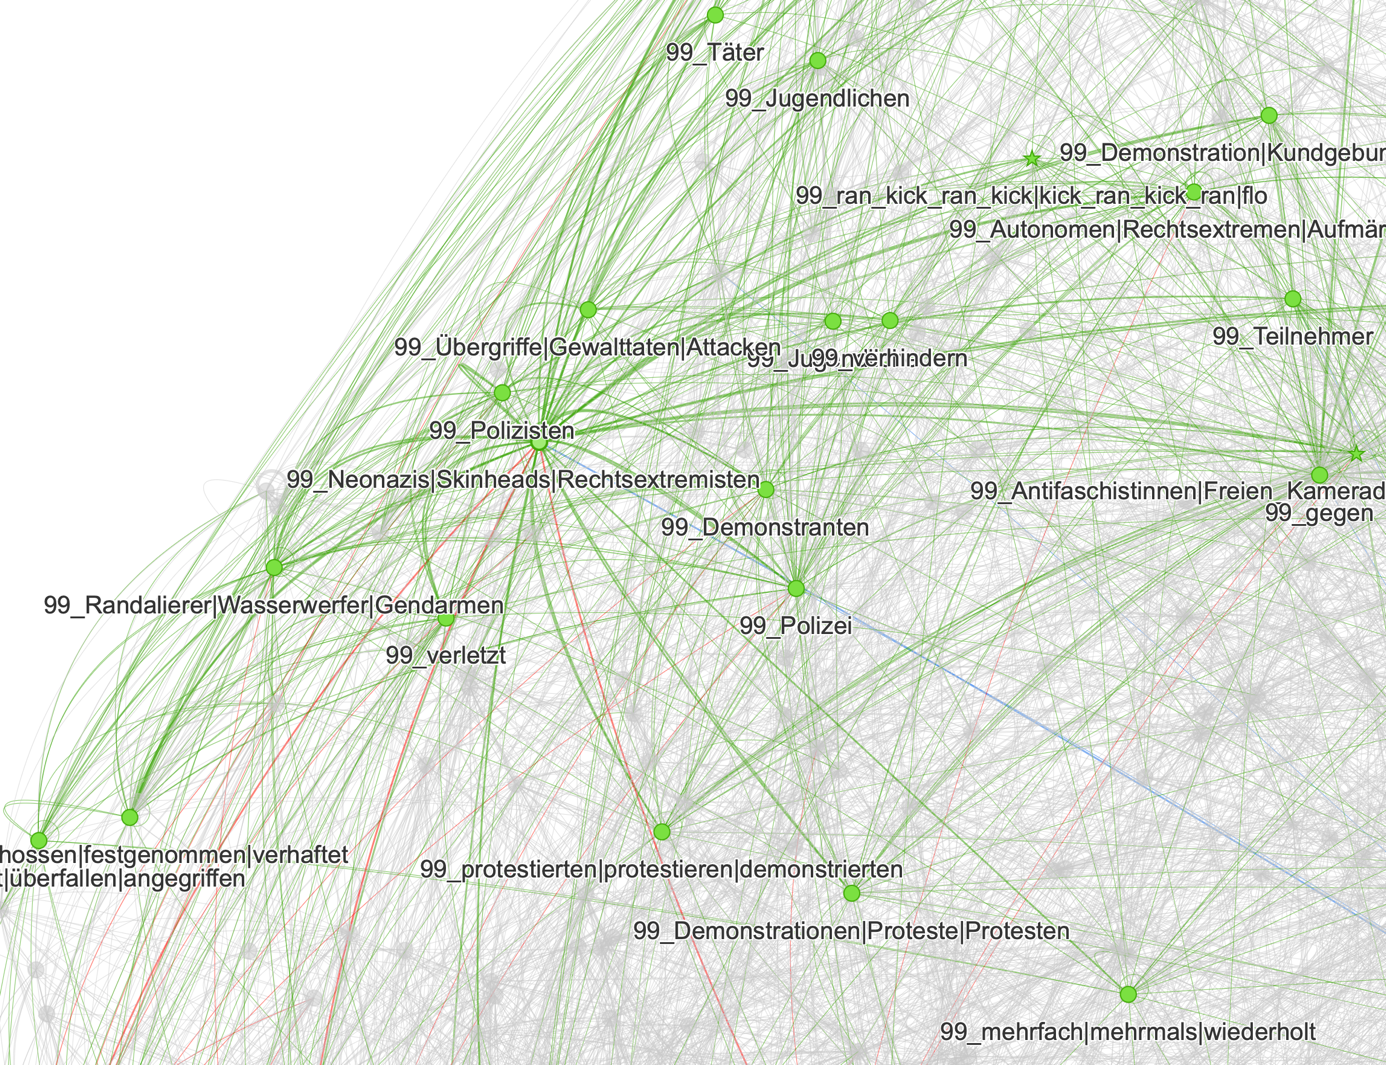
\includegraphics[width=\textwidth]{figures/media/image31.png}
  \caption{\label{fig:perspektivierung-neonazis}Perspektivierung rechtsextremistischer Akteure durch das FE \cluster{99\_Neonazis{\breakbar}Skinheads{\breakbar}Rechtsextremisten}.}
\end{figure}

Das Cluster \cluster{99\_Neonazis{\breakbar}Skinheads{\breakbar}Rechtsextremisten}, das außer den namensgebenden Wörtern auch die Ausdrücke \emph{Polizeisprecher}, \emph{Aktivisten}, \emph{Sicherheitskräfte}, \emph{Ausschreitungen}, \emph{nach\_Polizeiangaben}, \emph{Hooligans}, \emph{Polizeibeamte} und \emph{Festnahmen} umfasst, und insofern neben rechtsextremen Akteuren auch andere an Demonstrationen beteiligte Akteure sowie einzelne assoziierte Handlungen enthält, ist hingegen im Bereich des der ‚Straftaten \& des Juristischen` zu verorten (siehe \figref{fig:perspektivierung-neonazis}). Es zeigt sich dabei ein Framing, das insbesondere gewaltvolles Handeln (u.\,a. \cluster{99\_verletzt}, \cluster{99\_vergewaltigt{\breakbar}überfallen{\breakbar}angegriffen}, \cluster{99\_Übergriffe{\breakbar}Gewalttaten{\breakbar}Attacken}) und seine Verfolgung (u.\,a. \cluster{99\_Tat}, \cluster{99\_Täter}, \cluster{99\_Polizei}, \cluster{99\_Beamten{\breakbar}Beamte}) sowie Demonstrationen (u.\,a. \cluster{99\_Demonstranten}, \cluster{99\_demonstrationen{\breakbar}Proteste{\breakbar}Protesten}) und Organisiertheit (u.\,a. \cluster{99\_Teilnehmer}, \cluster{99\_Gruppe}, \cluster{99\_Autonomen{\breakbar}Rechtsextremen{\breakbar}Aufmärsche}) in den Vordergrund stellt. Dass etwa der syntagmatische Bezug zu Gewalt und Strafverfolgung der Wörter des Clusters nicht nur auf die enthaltenen Wörter wie \emph{Polizeibeamte} oder \emph{Festnahmen} zurückgeht, die ja auch außerhalb rechtsextremistischer Kontexte vorkommen können, lässt sich zeigen, indem (\emph{corpus-based}) die Kollokationen einzelner Wörter nachgeprüft werden. Das Wort \emph{Skinheads} etwa, das in diesem Zeitraum -- wie im Tooltipp zum Knoten ersichtlich -- in Bezug auf seine Keyness hochsignifikant (626,7 \emph{Log-Likelihood}) ist, hat unter seinen 50 Top-Kollokaten Wörter wie \emph{überfallen}, \emph{angepöbelt}, \emph{festgenommen}, \emph{Baseballschläger}, \emph{schlugen} oder \emph{Tode\_geprügelt}, was den Zusammenhang der rechtsextremen Akteure mit Gewalttaten und ihrer Ermittlung vereindeutigt.
\largerpage[-1]

\begin{figure}[t]
  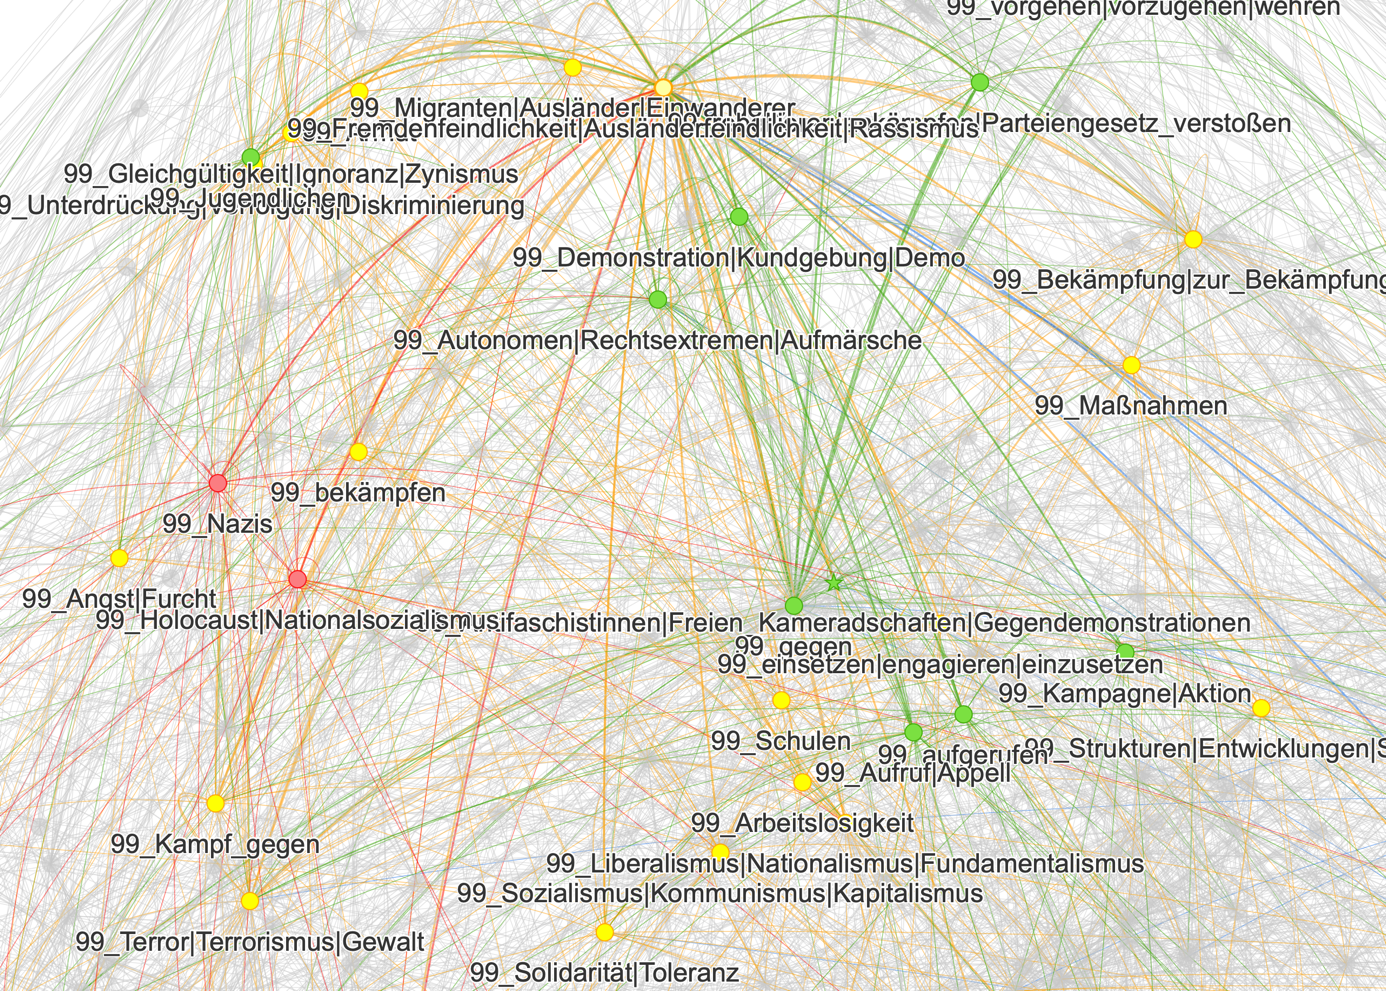
\includegraphics[width=\textwidth]{figures/media/image32.png}
  \caption{\label{fig:xenophobie-rassismus}Perspektivierung des Rechtsextremismus-Frames durch das FE \cluster{99\_Fremdenfeindlichkeit{\breakbar}Ausländerfeindlichkeit{\breakbar}Rassismus}.}
\end{figure}

Als letztes Cluster dieses Varianten-Frames soll das im thematischen Bereich ‚Staat, FdGO \& Gesellschaft` angesiedelte FE \cluster{99\_Fremdenfeindlichkeit{\breakbar}Ausländerfeindlichkeit{\breakbar}Rassismus (Charakteristika des Rechtsextremismus)} in den Blick genommen werden (\figref{fig:xenophobie-rassismus}). Wird dieses FE evoziert, treten erneut gänzlich andere Bedeutungsanteile des Rechtsextremismus-Frames in den Vordergrund. Angeschlossene FE wie \cluster{99\_Maßnahmen}, \cluster{99\_einsetzen{\breakbar}engagieren{\breakbar}einzusetzen}, \cluster{99\_Bekämpfung{\breakbar}zur\_Bekämpfung}, \cluster{99\_Mittel}, \cluster{99\_Kampf\_gegen} stellen Rechtsextremismus und seine Eigenschaften ein zu bekämpfendes Problem heraus. Es ist darüber hinaus mit anderen gesellschaftlichen Problemen wie \cluster{99\_Armut} oder \cluster{99\_Arbeitslosigkeit} verbunden, wobei eine Sichtung der entsprechenden Belegstellen zeigt, dass diese sowohl als Ursachen als auch als assoziierte kontige Konzepte zu lesen sind. Sie werden dabei oft in konjunktiv verknüpften Aufzählungen realisiert (siehe Belege K02--K04 in \tabref{tab:K02-K04}).

\begin{table}
  \caption{Konkordanzen zur Kollokation der Cluster \cluster{99\_Arbeitslosigkeit} und \cluster{99\_Fremdenfeindlichkeit{\breakbar}Ausländerfeindlichkeit{\breakbar}Rassismus}.}
  \label{tab:K02-K04}
K02 taz\_368196
\begin{tabularx}{\textwidth}{QQQ}
\toprule
noch private Niederlagen und Demütigungen wie die Scheidung von seiner Frau dazu dann Wende und & {[}\cluster{99\_Arbeitslosigkeit}: \textbf{Arbeitslosigkeit}{]}\newline
\textbf{und}\newline
{[}\cluster{99\_Fremdenfeindlichkeit{\breakbar}Ausländerfeindlichkeit{\breakbar}Rassismus:} \textbf{Ausländerfeindlichkeit}{]} & das volle\_Programm und im Mauerschützenprozess wird ausgerechnet sein inzwischen erwachsener Mannschaftskapitän angeklagt Heiko armer kleiner \\
\bottomrule
\end{tabularx}
\bigskip \newline
K03 taz\_92529
\begin{tabularx}{\textwidth}{QQQ}
\toprule
die innenpolitische\_Lage die Zuwanderung erwünscht oder unerwünscht macht bestenfalls heimlich und hinter\_vorgehaltener\_Hand diskutiert ich\_glaube dass & {[}\cluster{99\_Arbeitslosigkeit}: \textbf{Arbeitslosigkeit}{]}\newline
\textbf{und}\newline
{[}\cluster{99\_Fremdenfeindlichkeit{\breakbar}Ausländerfeindlichkeit{\breakbar}Rassismus:} \textbf{Ausländerfeindlichkeit}{]} & Argumente sein können den Ausländerzuzug zu drosseln braucht Deutschland ein Einwanderungsgesetz ja ich\_denke dass wir \\
\bottomrule
\end{tabularx}
\bigskip \newline
K04 welt\_26766
\begin{tabularx}{\textwidth}{QQQ}
\toprule
neuen Liberalismus der all\_jenen zugute\_kommen soll über die der Wirtschaftsboom der neunziger\_Jahre hinweggegangen ist dem & {[}\cluster{99\_Fremdenfeindlichkeit{\breakbar}Ausländerfeindlichkeit{\breakbar}Rassismus:} \textbf{Rassismus}{]}\newline
\textbf{und der}\newline
{[}\cluster{99\_Armut}: \textbf{Armut}{]} & in Amerika will er den Kampf\_ansagen und eine Krankenversicherung für alle Amerikaner schaffen große Aufgaben \\
\bottomrule
\end{tabularx}
\end{table}

Einige Cluster lassen sich weder eindeutig rechten noch linken extremistischen Bewegungen zuordnen und bilden so einen variantenübergreifenden Frame des politischen Extremismus. Der bereits skizzierte Rechtsextremismus-Frame kann im Sinne eines rekursiven Frame-Modells auch als Teil dieses Frames betrachtet werden. Einschlägig ist dabei insbesondere das Cluster \cluster{99\_Autonomen{\breakbar}Rechtsextremen{\breakbar}Aufmärsche (Politischer Extremismus \& Protest)}.\footnote{Ein weiteres Cluster \cluster{99\_Antifaschistinnen{\breakbar}Freien\_Kameradschaften{\breakbar}Gegendemonstrationen} erscheint zwar ebenfalls zu diesem Bereich gehörig -- und dies trifft auf eine Vielzahl der beinhalteten Wörter auch zu -- ist aber mit 254 enthaltenen Wörtern relativ groß und semantisch heterogen, sodass es nicht weiter ausgewertet wird.} Seine Relationen im Frame liegen größtenteils im thematischen Bereich ‚Straftaten \& Juristisches`, wo es ähnliche Verbindungen ausprägt wie das bereits besprochene Cluster \cluster{99\_Neonazis{\breakbar}Skinheads{\breakbar}Rechtsextremisten}, sodass Gewalt und Demonstrationen auch hier Teil des Framings sind. Die gewaltbezogenen FE unterscheiden sich jedoch insofern als besonders schwere Straftaten wie \cluster{99\_vergewaltigt{\breakbar}überfallen{\breakbar}angegriffen} hier nicht mehr assoziiert sind. Eine Sichtung der Konkordanzen zur Kookkurrenz mit dem Cluster \cluster{99\_Übergriffe{\breakbar}Gewalttaten{\breakbar}Attacken} wiederum macht deutlich, dass es dabei in der großen Mehrzahl um rechte Gewalt, oft gegen linke Akteure, geht. Es finden sich darüber hinaus Verbindungen in die Netzwerk-Community Politik mit FE wie \cluster{99\_Widerstand}, \cluster{99\_Vereine{\breakbar}Verbände{\breakbar}Vereinen} und in den Bereich ‚Staat, FdGO \& Gesellschaft` mit FE wie \cluster{99\_Organisationen{\breakbar}Initiativen{\breakbar}Institutionen} oder \cluster{99\_Bewegung}, die ebenfalls auf die Organisiertheit Bezug nehmen, jedoch dabei eine stärker legitimierende Perspektivierung andeuten als die äquivalenten FE im Rechtsextremismus-Frame.

\subsubsection{Islamismus}\label{islamismus}

Für den Islamismus-Frame erscheinen die folgenden FE besonders einschlägig, die alle im thematischen Teil-Frame ‚Krieg \& Islamismus` zu finden sind: \cluster{99\_Hebron{\breakbar}jüdische\_Siedler{\breakbar}israelischen\_Armee} \cluster{(Nahostkonflikt)}, \cluster{99\_Israelis{\breakbar}Palästinenser{\breakbar}Palästinensern (Bevölkerungsgruppen Nahostkonflikt)}, \cluster{99\_Islamisten{\breakbar}islamistischen{\breakbar}Pkk (extremistische Gruppierungen im Ausland, insb. Islamismus)}, \cluster{99\_Taliban}, \cluster{99\_Terroristen{\breakbar}Bin\_Laden{\breakbar}Waffen (Terroristen{\slash}Waffen)} und \cluster{Hussein{\breakbar}Abu{\breakbar}Ahmed} \cluster{(terroristische bzw. diktatorische Akteure)}.

Die beiden FE, die auf den Nahostkonflikt Bezug nehmen, werden durch angeschlossene Cluster wie u.\,a. \cluster{99\_getötet}, \cluster{99\_Bombe{\breakbar}Detonation{\breakbar}Sprengsatz (Attentate)}, \cluster{99\_verletzt\_worden} als gewaltvoller Konflikt geframet, der durch kriegerische Handlungen und Attentate geführt wird. FE aus dem Netzwerk-Cluster ‚Politik` wie \cluster{99\_Scharon{\breakbar}Barak{\breakbar}Arafat}, \cluster{99\_Besuch} und \cluster{99\_Gipfel{\breakbar}Gipfeltreffen{\breakbar}EU-gipfel} sowie aus dem Bereich ‚Staat, FdGO \& Gesellschaft` wie \cluster{99\_Umsetzung}, \cluster{99\_Verhandlungen{\breakbar}Gespräche} zeigen zudem die diplomatischen Bemühungen zur Lösung des Konfliktes an.

Die drei weiteren identifizierten FE und die an sie angeschlossenen FE tragen ebenfalls zu einem Framing von Islamismus bei, das durch kriegerische Handlungen und Attentate im Ausland markiert ist (\cluster{99\_Bombenangriffe{\breakbar}Bombardements{\breakbar}Bombardierungen}, \cluster{99\_Irak}, \cluster{99\_Nordkorea{\breakbar}Libyen{\breakbar}Syrien}) und bei dem nicht nur Staaten, sondern auch einzelne extremistische Gruppierungen eine Rolle spielen: \cluster{99\_Islamisten{\breakbar}islamistischen{\breakbar}Pkk} \cluster{(islamistische Akteure, aber auch Akteure des auslandsbezogenen Extremismus wie \emph{Eta} und \emph{Pkk})}, \cluster{99\_Rebellen}, \cluster{99\_Taliban} und weitere. Die Anschläge vom 11. September 2001 sind in diesem Zeitraum noch nicht deutlich im Frame sichtbar, was vermutlich darauf zurückgeht, dass sie erst gegen Ende dieses zeitlichen Abschnittes stattgefunden haben. Weitere epistemische Spezifizierungen finden sich in den anderen thematischen Frame-Teilen: Das Cluster ‚Staat, FdGO \& Gesellschaft` hebt einerseits den Aspekt der Zugehörigkeit, der im Islamismus-Frame durch Fragen der Religion und Herkunft eine besondere Rolle spielt, hervor (\cluster{99\_christlichen{\breakbar}religiösen{\breakbar}christliche}, \cluster{99\_Einheit{\breakbar}Nation{\breakbar}Gemeinschaft}, \cluster{99\_Identität{\breakbar}Herkunft}) und konstitutiert Islamismus andererseits als zu bekämpfendes Phänomen (\cluster{99\_Kampf\_gegen}, \cluster{99\_bekämpfen}). Im thematischen Teil-Frame ‚Politik` schlagen sich neben politischen Akteuren (u.\,a. \cluster{99\_Scharon{\breakbar}Barak{\breakbar}Arafat}, \cluster{99\_Präsident\_Bill\_Clinton{\breakbar}Bill\_Clinton{\breakbar}Us-präsident\_George\_W\_Bush}) auch Fragen der Anhängerschaft (u.\,a. \cluster{99\_Mitgliedern}, \cluster{99\_Anhänger{\breakbar}Gegner}, \cluster{99\_Vereine{\breakbar}Verbände{\breakbar}Vereinen}) nieder.

\subsubsection{Fazit}\label{fazit}

Insgesamt zeigen sich in diesem Zeitraum deutliche Unterschiede zwischen dem Framing von politischem Extremismus und Islamismus. Bei ersterem ist nur der Rechtsextremismus epistemisch ausdifferenziert im Frame angelegt. Es finden sich eigene Cluster zu Akteuren, dem Nationalsozialismus sowie zu Charakteristika dieser Extremismusform, wohingegen linksextreme Akteure oder Handlungen nur gemeinsam mit solchen des Rechtsextremismus in Clustern zusammengefasst vorkommen. Dies deutet an, dass Linksextremismus in diesem Zeitraum kein frequent thematisiertes oder deutlich divergent geframetes Phänomen darstellt, was sich damit deckt, dass in den entsprechenden Clustern Ausdrücke wie \emph{Rechtsextremismus} (1686 Vorkommen) oder \emph{Rechtsextremisten} (819 Vorkommen) um ein Vielfaches häufiger auftreten als etwa die jeweils 83 Mal vorkommenden Ausdrücke \emph{Linksextremismus} und \emph{Linksextremisten}. Dass sich auch bei mitunter geteilten Clustern dennoch ein eigener Rechtsextremismus-Frame abgrenzen lässt, zeigt, dass beide Extremismusvarianten zwar in Teilen ein ähnliches Framing, jedoch im Falle des Rechtsextremimus auch Alleinstellungsmerkmale aufweisen. Diese bestehen insbesondere im historischen Bezug der auf den Zweiten Weltkrieg verweisenden FE, dem FE der in einem Verbotsverfahren begriffenen NPD sowie den attributiven Zuschreibungen an Rechtsextremismus, die ebenfalls in einem FE organisiert sind. Als geteilte Merkmale des politischen Extremismus in diesem Zeitraum tritt insbesondere die Praktik des Demonstrierens und die Organisiertheit hervor. Letztere und auch die Assoziation mit Gewalt haben jedoch eine andere Qualität als im Rechtsextremismus-Frame und werden nicht gleichermaßen negativ perspektiviert.

Der Islamismus-Frame ist ebenfalls stark durch gewaltvolles Handeln geprägt. Dieses wird jedoch in Form von kriegerischen Handlungen und Attentaten realisiert, u.\,a. im Nahostkonflikt. Es finden sich hier einzelne FE, die auch Akteure des sogenannten auslandsbezogenen Extremismus abbilden wie die PKK oder ETA. Weiterhin finden sich auf Akteursebene politische Akteure wie Präsidenten der USA oder Israels und Terrororganisationen wie die Taliban.

\subsection{Der Zeitraum 2002--2004}\label{der-zeitraum-2002-2004}

\subsubsection{\texorpdfstring{\emph{Corpus-driven} Voranalyse: Thematisch gruppierte Auswahl semantisch äquivalenter Cluster im Vergleich zu den Kern-FE des vorigen Zeitraums}{Corpus-driven Voranalyse: Thematisch gruppierte Auswahl semantisch äquivalenter Cluster im Vergleich zu den Kern-FE des vorigen Zeitraums}}\label{corpus-driven-voranalyse-thematisch-gruppierte-auswahl-semantisch-aequivalenter-cluster-im-vergleich-zu-den-kern-fe-des-vorigen-zeitraums}

Um Kandidaten für die im Zeitraum 2002--2004 für den politischen Extremismus relevanten FE zu identifizieren, wurden zunächst die im Vektorraum in der Nähe der Cluster des vorigen Zeitraums befindlichen Cluster ermittelt. Tabelle 3 im Anhang zeigt pro Cluster des Zeitraumes 1999--2001 die fünf Cluster im Zeitraum 2002--2004 mit der höchsten Cosinus-Ähnlichkeit. Die Ergebnisse zeigen, dass einige FE des Zeitraumes 1999--2001 sehr äquivalente FE mit teils großen lexikalischen Überlappungen im Folgezeitraum aufweisen, was durch hohe Cosinus-Ähnlichkeitswerte von 0,85 und höher quantitativ unterlegt ist. Beispiele hierfür sind die Äquivalenzen \cluster{99\_NPD} zu \cluster{02\_NPD (0.91)}, \cluster{99\_Holocaust{\breakbar}Nationalsozialismus} zu \cluster{02\_Holocaust{\breakbar}Nazis{\breakbar}Nationalsozialismus (0.88)} oder \cluster{99\_Israelis{\breakbar}Palästinenser{\breakbar}Palästinensern} zu \cluster{02\_Israelis{\breakbar}Palästinenser{\breakbar}Palästinensern (0.97)}. Dass das letztgenannte Cluster einen besonders hohen Wert erreicht, kann nicht unmittelbar durch die lexikalische Identität mit dem äquivalentesten Cluster im Vorjahreszeitraum erklärt werden. Schließlich ist auch das Cluster \cluster{02\_Npd} lexikalisch identisch mit \cluster{99\_Npd}, jedoch nicht gleichermaßen nah positioniert. Ausdrucksseitige Identität ist natürlich ein starker Hinweis auf Bedeutungsähnlichkeit, diese zu fokussieren verstellt aber den Blick darauf, dass Wörter ihre Bedeutung ständig auf subtile Art und Weise wandeln und -- Frame-semantisch gesprochen -- zumindest graduell andere Frames evozieren. Dies gilt zumindest, wenn man das gesamte verstehensrelevante Wissen anstatt eines enggefassten Bedeutungskonzeptes zugrunde legt.

Unter den so gesammelten Clustern verweisen die Cluster in \tabref{tab:2002} vergleichsweise eindeutig auf den Extremismusdiskurs, was von diesem Zeitraum an also zusätzlich durch die Ähnlichkeit der linguistischen Kontexte, in denen sie im Vergleich zum vorgängigen Zeitraum vorkommen, empirisch-datengeleitet unterlegt wird. Sie sind darüber hinaus nach Extremismusvariante sowie einzelnen Teil-Frames, die sich herausbilden, gruppiert.

\begin{table}\small
\caption{Thematisch gruppierte Auswahl semantisch äquivalenter Cluster des Zeitraums 2002--2004.}
\label{tab:2002}
 \begin{tabularx}{\textwidth}{>{\hsize=0.5\hsize}X >{\hsize=0.5\hsize}X >{\hsize=2.0\hsize}X}
  \lsptoprule
  Extremismus-Variante & Bezug & Frame-Elemente \\
  \midrule
  \multirow{2}{=}{Rechts\-ex\-tre\-mis\-mus} 
  & historisch & \cluster{Holocaust{\breakbar}Nazis{\breakbar}Nationalsozialismus, Ss{\breakbar}Nazi-deutschland{\breakbar}Nazi-zeit, 1945{\breakbar}Zweiten\_Weltkrieg} \\
  & zeit\-ge\-nössisch & \cluster{Npd, Antisemitismus, Intoleranz{\breakbar}Hetze{\breakbar}Rassismus} \\
  \midrule
  Links\-ex\-tre\-mis\-mus & zeit\-ge\-nössisch & \cluster{Pds} \\
  \midrule
  \multirow{2}{=}{Politischer Extremismus} 
  & historisch & \cluster{Weimarer\_Republik{\breakbar}Nationalsozialisten{\breakbar}Sowjetunion, Liberalismus{\breakbar}Nationalismus{\breakbar}Totalitarismus} \\
  & zeit\-ge\-nössisch & \cluster{Autonomen{\breakbar}Antifa{\breakbar}Rechtsextremisten, Schill-Partei{\breakbar}Schill{\breakbar}GAL} \\
  \midrule
  {Islamismus} & Nahost\-konflikt & \cluster{Tulkarm{\breakbar}Tulkarem{\breakbar}jüdische\_Siedler, Hebron{\breakbar}Nablus{\breakbar}Rafah, Palästinenserpräsident\_Jassir\_Arafat{\breakbar}Jassir\_Arafat{\breakbar}Abbas, Gaza{\breakbar}Ramallah{\breakbar}Tel\_Aviv, Gaza-streifen{\breakbar}Westjordanland{\breakbar}Gazastreifen, Israelis{\breakbar}Palästinenser{\breakbar}Palästinensern, israelischen{\breakbar}israelische{\breakbar}palästinensische} \\
  & Irakkrieg & \cluster{Al\_Qaida{\breakbar}al-Qaida{\breakbar}Extremisten, Qaida{\breakbar}Terrorgruppe{\breakbar}Terrororganisation, Taliban-Kämpfer{\breakbar}Al-Qaida-Kämpfer{\breakbar}Afghanen, Saddam\_Hussein{\breakbar}Saddam} \\
  \lspbottomrule
 \end{tabularx}
\end{table}

\subsubsection{\texorpdfstring{\emph{Corpus-driven} Voranalyse: Cluster mit hoher Cosinus-Distanz im Vergleich zum vorigen Zeitraum}{Corpus-driven Voranalyse: Cluster mit hoher Cosinus-Distanz im Vergleich zum vorigen Zeitraum}}\label{corpus-driven-voranalyse-cluster-mit-hoher-cosinus-distanz-im-vergleich-zum-vorigen-zeitraum}

Als weiteres datengeleitetes Element, das die Analyse informieren kann, werden erneut die 20 Cluster berechnet, die die größte Cosinus-Distanz im Vektorraum zurückgelegt haben. In den so ermittelten Clustern zeichnen sich mehrere in diesem Zeitraum relevante Themen ab (siehe \tabref{tab:cluster-high-cosine-distance-2002}). Cluster wie \cluster{02\_Bösen{\breakbar}Achse}, \cluster{02\_Iraker}, \cluster{02\_Us-soldaten}, \cluster{02\_Inspektionen{\breakbar}Waffeninspektionen{\breakbar}Waffeninspektoren} verweisen auf den im Jahr 2003 durch die USA und Großbritannien geführten Irak-Krieg. Der Krieg wurde insbesondere mit der Vermutung von Massenvernichtungswaffen im Irak begründet; ein Topos, der bereits im Januar 2002, in Folge der Anschläge vom 11. September, durch George W. Bush prominent in die Debatte eingebracht wurde. Seine Prägung des Begriffs der ‚Achse des Bösen` schlägt sich dabei an erster Stelle in den gelisteten Clustern nieder. Des Weiteren spiegelt sich die sogenannte Möllemann-Affäre, in der ihm Antisemitismus bzw. Israel-Feindlichkeit vorgeworfen wird, in der Auflistung wider (\cluster{02\_Jürgen\_Möllemann}{\breakbar}\cluster{Hohmann}{\breakbar}\cluster{Möllemanns}, \cluster{02\_Möllemann{\breakbar}Westerwelle}).

\begin{table}[t]\small
\caption{Cluster mit hoher Cosinus-Distanz im Vergleich zum vorigen Zeitraum.}
\label{tab:cluster-high-cosine-distance-2002}
\begin{tabularx}{\textwidth}{X r}
\lsptoprule
Cluster & Cos.-Dist. \\
\midrule
\cluster{Bösen{\breakbar}Achse} & 0.41 \\
\cluster{Sarrazin{\breakbar}Strieder{\breakbar}Wowereit} & 0.31 \\
\cluster{Iraker} & 0.29 \\
\cluster{Demokraten{\breakbar}Republikaner{\breakbar}Kerry} & 0.29 \\
\cluster{Jürgen\_Möllemann{\breakbar}Hohmann{\breakbar}Möllemanns} & 0.27 \\
\cluster{Irak} & 0.24 \\
\cluster{Riester{\breakbar}Hartz{\breakbar}Rürup} & 0.23 \\
\cluster{Saddam\_Hussein{\breakbar}Saddam} & 0.22 \\
\cluster{Münteferings{\breakbar}Merkels{\breakbar}Fischers} & 0.21 \\
\cluster{Us-soldaten} & 0.21 \\
\cluster{Saddam\_Husseins{\breakbar}Saddams{\breakbar}Hussein} & 0.21 \\
\cluster{schiitischen{\breakbar}sunnitischen{\breakbar}al-Sadr} & 0.21 \\
\cluster{Inspektionen{\breakbar}Waffeninspektionen{\breakbar}Waffeninspektoren} & 0.2 \\
\cluster{Bagdad} & 0.2 \\
\cluster{Innensenator{\breakbar}Innensenator\_Ronald\_Schill{\breakbar}kusch} & 0.19 \\
\cluster{Csu-landesgruppenchef\_Michael\_Glos{\breakbar}Grünen-chef\_Reinhard\_Bütikofer{\breakbar}Stiegler} & 0.19 \\
\cluster{Rüttgers{\breakbar}Wulff{\breakbar}Steinbrück} & 0.19 \\
\cluster{irakischen{\breakbar}irakische} & 0.19 \\
\cluster{Möllemann{\breakbar}Westerwelle} & 0.18 \\
\cluster{RCD{\breakbar}Kongos{\breakbar}Ruandas} & 0.18 \\
\lspbottomrule
\end{tabularx}
\end{table}

\subsubsection{Rechts- und Linksextremismus}\label{rechts--und-linksextremismus-1}

Einen wesentlichen Teil des Rechtsextremismus-Frames macht erneut die Zeit des Nationalsozialismus aus. Die Cluster \cluster{02\_Ss{\breakbar}Nazi-deutschland{\breakbar}Nazi-zeit}, \cluster{02\_Holocaust{\breakbar}Nazis{\breakbar}Nationalsozialismus} und \cluster{02\_1945{\breakbar}Zweiten\_Weltkrieg} prägen primär Frame-Relationen im Bereich ‚Krieg \& Islamismus` aus, die die Gräueltaten dieser Zeit (\cluster{02\_Massakern{\breakbar}Gräueltaten{\breakbar}Morden (Krieg \& Gräueltaten)}, \cluster{02\_Überlebende{\breakbar}Opfern{\breakbar}Überlebende}, \cluster{02\_Flucht}, \cluster{02\_Schicksal{\breakbar}Leid}) sowie das Erinnern an ebendiese (\cluster{02\_Jahrestag}) abbilden. Im thematischen Teil-Frame ‚Staat, FdGO \& Gesellschaft` emergieren darüber hinaus FE, die den Bezug zur deutschen Gesellschaft (\cluster{02\_Schuld}, \cluster{02\_Deutschen}, \cluster{02\_Vorfahren{\breakbar}Nachfahren{\breakbar}Nachkommen}) herstellen.

Das Framing der NPD speist sich durch das noch immer laufende Verbotsverfahren weiterhin aus den Bereichen ‚Politik` sowie ‚Straftaten \& Juristisches` und hat sich dabei nicht wesentlich verändert. Charakteristika des Rechtsextremismus spiegeln sich in diesem Zeitraum in den Clustern \cluster{02\_Antisemitismus} und \cluster{02\_Intoleranz{\breakbar}Hetze{\breakbar}Rassismus} wider. Letzteres ist im Vergleich zum Vorjahreszeitraum semantisch etwas weiter gefasst und beinhaltet auch Wörter wie \emph{Hetze}, \emph{Homosexuelle} oder \emph{Zensur}, also einzelne Mittel der Unterdrückung bzw. diskriminierte Gruppen. Mit diesen FE verbunden findet sich als neues Element des Framings nun die von Antisemitismusvorwürfen geprägte Möllemann-Affäre (\cluster{02\_Möllemann{\breakbar}Westerwelle}, \cluster{02\_Jürgen\_Möllemann{\breakbar}Hohmann{\breakbar}Möllemanns}), die bereits in der \emph{corpus-driven} Analyse zum Bedeutungswandel aufgefallen war.

In der Voranalyse zur semantischen Äquivalenz wurde zudem das FE \cluster{02\_Schill-Partei{\breakbar}Schill{\breakbar}GAL} als äquivalent zum FE \cluster{99\_NPD} identifiziert (siehe Tabelle 3 im Anhang). Es umfasst die Hamburger Parteien ‚Partei Rechtsstaatlicher Offensive` (auch als \emph{Schill-Partei} bezeichnet) und die Grünen, deren Hamburger Landesverband zu der Zeit ‚Grün-Alternative Liste` (\emph{GAL}) hieß. Im Framing der Parteien werden jedoch kaum FE mit engerem thematischem Bezug zu Extremismus augenscheinlich. Auffällig ist, dass das FE fast ausschließlich im Bereich ‚Politik` vernetzt ist, jedoch mit \cluster{02\_Waffe} auch ein FE aus der Community ‚Krieg \& Islamismus` anbindet. Dies geht auf die mediale Diskussion um den Umstand, dass der rechtspopulistische damalige Innensenator \emph{Schill} eine \emph{Waffe} zur Selbstverteidigung bei sich trug, zurück.

\begin{figure}
  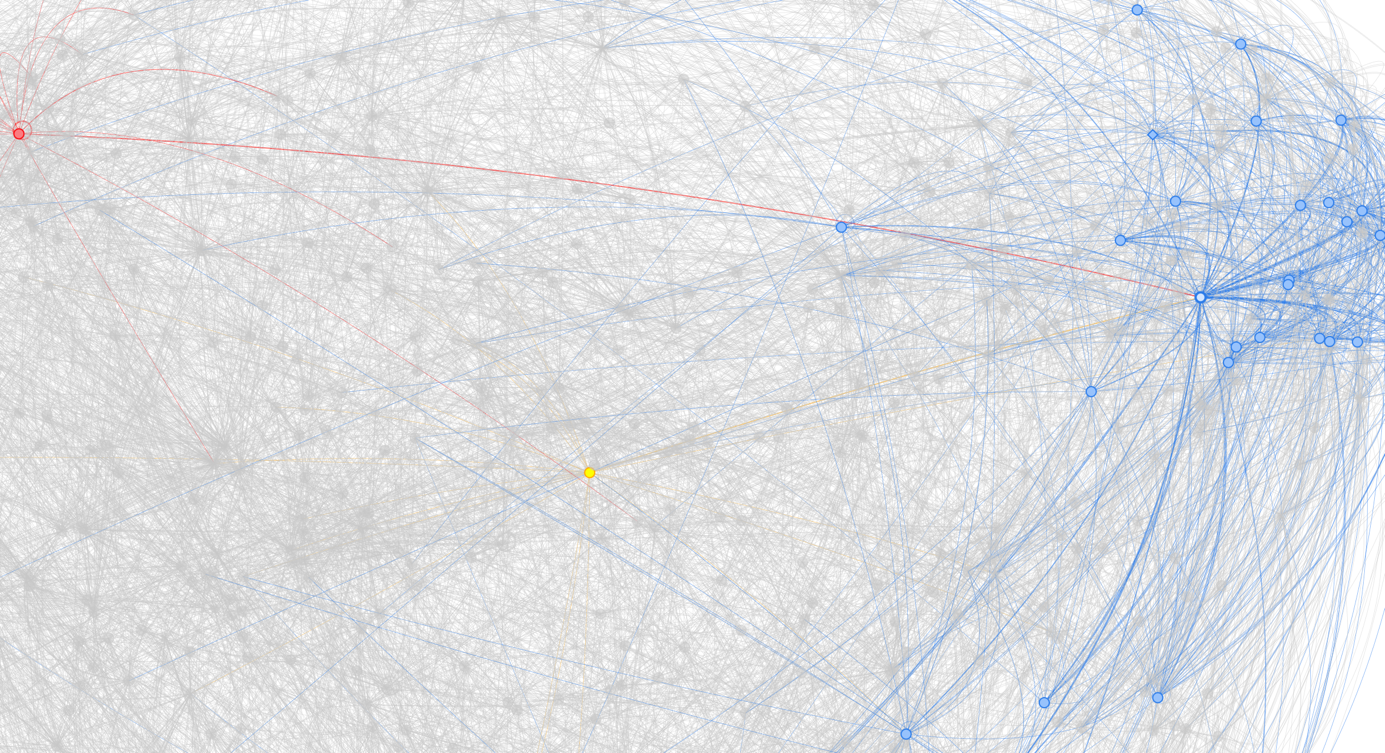
\includegraphics[width=\textwidth]{figures/media/image33.png}
  \caption{\label{fig:pds-vernetzung}Vernetzung des FE \cluster{02\_Pds} (rechts) im Gesamt-Frame.}
\end{figure}
\newpage
Als Partei am linksäußeren Rand, die zudem als bedeutungsähnlich zur NPD im vorangehenden Zeitraum identifiziert wurde (siehe Tabelle 3 im Anhang), soll das FE \cluster{02\_Pds} als Teil eines Linksextremismus-Frames in den Blick genommen werden. Wie in \figref{fig:pds-vernetzung} ersichtlich, ist das FE fast ausschließlich im thematischen Bereich der Innenpolitik vernetzt, wobei insbesondere die Anbindung an die FE \cluster{02\_Npd} und \cluster{02\_Autonomen{\breakbar}Antifa{\breakbar}Rechtsextremisten (politischer Extremismus)} ein Framing als extremistische Partei andeuten. Das FE \cluster{02\_Norden{\breakbar}Süden{\breakbar}Osten} aus der Community ‚Krieg \& Islamismus` (links in der Abbildung) verweist außerdem auf den regional begrenzten Erfolg der Partei. Auch das angebundene FE \cluster{02\_Zusammenarbeit{\breakbar}Kooperation} aus dem Bereich ‚Staat, FdGO \& Gesellschaft` (in der Mitte der Abbildung) zeigt eine besondere Rolle der PDS im Parteienspektrum an, da in Frage steht, inwiefern eine Zusammenarbeit in einer Koalition, wie sie in Berlin auf Landesebene seit 2001 besteht, gerechtfertigt ist (siehe Belege K05--K07 in \tabref{tab:K05-K07}).

\begin{table}
\caption{Konkordanzen zur Kollokation der Cluster \cluster{02\_Pds} und \cluster{02\_Zusammenarbeit{\breakbar}Kooperation}.}
\label{tab:K05-K07}
K05 spiegel\_461705
\begin{tabularx}{\textwidth}{QQQ}
\toprule
und Csu-chef\_Stoiber lehnten eine große\_Koalition nach der Wahl am lt100 September ab Schröder schloss eine & {[}\cluster{02\_Zusammenarbeit{\breakbar}Kooperation}: \textbf{Zusammenarbeit}{]}\newline
\textbf{mit der}\newline
{[}\cluster{02\_Pds}: \textbf{Pds}{]} & aus in dem Fernsehduell flammte der Streit über die Finanzierung des Wiederaufbaus nach der Flut \\
\bottomrule
\end{tabularx}
\bigskip \newline
K06 spiegel\_723618
\begin{tabularx}{\textwidth}{QQQ}
\toprule
alleinige\_Schuld an dem Wahldebakel in die Schuhe Matschie habe mit seiner sehr rigiden Ablehnung einer & {[}\cluster{02\_Zusammenarbeit{\breakbar}Kooperation}: \textbf{Zusammenarbeit}{]}\newline
\textbf{mit der}\newline
{[}\cluster{02\_Pds}: \textbf{Pds}{]} & die Wähler geradezu\_ermuntert den Linkssozialisten ihre Stimme zu geben sagte Dewes die Pds kam am\_Sonntag \\
\bottomrule
\end{tabularx}
\bigskip \newline
K07 taz\_795267
\begin{tabularx}{\textwidth}{QQQ}
\toprule
Liste aufstellen um bei dem Zugriffsverfahren auch Chancen zu haben eine andere Möglichkeit wäre die & {[}\cluster{02\_Zusammenarbeit{\breakbar}Kooperation}: \textbf{Kooperation}{]}\newline
\textbf{zwischen Fdp Bürgerbündnis und}\newline
{[}\cluster{02\_Pds}: \textbf{Pds}{]} & nur mit den Rechtsaußen will keiner die werden sich wohl wieder damit revanchieren dass sie \\
\bottomrule
\end{tabularx}
\end{table}

Das FE \cluster{02\_Autonomen{\breakbar}Antifa{\breakbar}Rechtsextremisten (Politischer Extremismus)} letztlich kondensiert als einziges FE neben den besprochenen Parteien den zeitgenössischen politischen Extremismus. Während dieser im Vorjahr noch in mehreren Clustern repräsentiert war und dabei ein von gewaltvollen Straftaten geprägtes Framing aufwies, sind in diesem Zeitraum der politische Bereich mit Bezügen zu Parteien (\cluster{02\_Parteien}, \cluster{02\_Pds}, \cluster{02\_Npd}), Gesetzen (\cluster{02\_Agenda\_2010{\breakbar}Reformen{\breakbar}Hartz\_Iv}) und Gewerkschaften (\cluster{02\_verdi{\breakbar}Dienstleistungsgewerkschaft\_Verdi{\breakbar}Gewerkschaft\_Verdi}) sowie zu Demonstrationen prägend. Dies geht auch auf die breite Semantik des Clusters, das mit 147 Wörtern sehr groß ist, zurück und etwa auch die \emph{Montagsdemonstrationen} gegen die Agenda 2010 umfasst, zurück. Ein extremistisches Framing manifestiert sich in den attributiven FE wie \cluster{02\_Intoleranz{\breakbar}Hetze{\breakbar}Rassismus} und \cluster{02\_Antisemitismus}, während Gewalt nur noch einen deutlich geringeren Teil des Frames ausmacht und sich etwa in den FE \cluster{02\_Randalierer{\breakbar}Wasserwerfer{\breakbar}Maschinenpistolen} und \cluster{02\_Razzien{\breakbar}Festnahmen{\breakbar}Verhaftungen} zeigt.

\subsubsection{Islamismus}\label{islamismus-1}

Für den Bereich des Islamismus liegt mit den datengeleitet identifizierten Clustern bereits eine Fülle an relevanten FE vor, die nur schlaglichtartig und in grundlegenden Tendenzen analysiert werden können.

Als Kernbestandteile des Frames werden die folgenden Cluster aufgefasst und an dieser Stelle bereits in Teil-Frames gegliedert: Einen Teil-Frame zum Nahostkonflikt bilden die FE \cluster{02\_Tulkarm{\breakbar}Tulkarem{\breakbar}jüdische\_Siedler (Nahostkonflikt)}, \cluster{02\_Hebron{\breakbar}Nablus{\breakbar}Rafah (Orte im Nahostkonflikt)}, \cluster{02\_Gaza{\breakbar}Ramallah{\breakbar}Tel\_Aviv (Orte im Nahostkonflikt \& israelische Armee)}, \cluster{02\_Gaza-streifen{\breakbar}Westjordanland{\breakbar}Gazastreifen (Orte im Nahostkonflikt)}, \cluster{02\_Israelis{\breakbar}Palästinenser{\breakbar}Palästinensern}, \cluster{02\_israelischen{\breakbar}israelische{\breakbar}palästinensische}, \cluster{02\_Palästinenserpräsident\_Jassir\_Arafat{\breakbar}Jassir\_Arafat{\breakbar}Abbas (Nahostkonflikt)}. Ein weiterer wesentlicher Teil des Islamismus-Frames umfasst FE, die mit den Anschlägen des 11. Septembers assoziiert sind. Hier finden sich die islamistische Gruppierungen Al-Qaida, die die Anschläge verübte sowie der Diktator Saddam Hussein, dem durch die USA Verbindungen zu Al-Qaida vorgeworfen wurde und dessen Sturz durch die USA im Rahmen des Irakkrieges forciert wurde: \cluster{02\_Al\_Qaida{\breakbar}al-Qaida{\breakbar}Extremisten (islamistische Akteure)}, \cluster{02\_Qaida{\breakbar}Terrorgruppe{\breakbar}Terrororganisation (terroristische Gruppen und Anschläge)}, \cluster{02\_Taliban-Kämpfer{\breakbar}Al-Qaida-Kämpfer{\breakbar}Afghanen (Akteure Islamismus)}, \cluster{02\_Saddam\_Hussein{\breakbar}Saddam}, \cluster{02\_Saddam\_Husseins{\breakbar}Saddams{\breakbar}Hussein}.

Der Nahostkonflikt wird insgesamt ähnlich geframet wie im vorigen Zeitraum. Es finden sich im Bereich ‚Krieg \& Islamismus` zahlreiche FE, die auf gewaltvolles kriegerisches Handeln sowie das Begehen von Anschlägen hindeuten. Die Communities ‚Innenpolitik` und ‚Außenpolitik` verdeutlichen dabei insbesondere diplomatische Bemühungen und die Community ‚Staat, FdGO \& Gesellschaft` darüber hinaus den durch Religion und terroristisches handeln geprägten Charakter des Konfliktes (\cluster{02\_Terrormis{\breakbar}Terror}, \cluster{02\_Juden}, \cluster{02\_Antismeitismus}, \cluster{02\_christliche{\breakbar}islamische{\breakbar}muslimische}, \cluster{02\_Moslems{\breakbar}Christen{\breakbar}Muslime}).

Am übrigen Teil des Islamismus-Frames, der das verstehensrelevante Wissen um den Irakkrieg und die Anschläge vom 11. September 2001 beinhaltet, sind insbesondere die Netzwerk-Cluster ‚Krieg \& Islamismus` sowie ‚Straftaten \& Juristisches` beteiligt. In ersterem tragen zum Islamismus-Framing FE, die den Irak bzw. das Regime Saddam Husseins als Ort bzw. Akteur des Krieges benennen, bei (u.\,a. \cluster{02\_Irak}, \cluster{02\_irakischen{\breakbar}irakische}, \cluster{02\_Saddam\_Husseins{\breakbar}Saddams{\breakbar}Hussein}, \cluster{02\_Regime}); zum anderen auch die durch die US-Regierung angeführte Begründung der Vermutung von Massenvernichtungswaffen (\cluster{02\_Massenvernichtungswaffen}, \cluster{02\_chemischen{\breakbar}chemische{\breakbar}Chemiewaffen (Chemiewaffen \& Atombombe)} und Kriegshandlungen (u.\,a. \cluster{02\_Anschläge{\breakbar}Attentate{\breakbar}Terroranschläge}, \cluster{02\_Attentäter{\breakbar}Selbstmordattentäter}, \cluster{02\_Angriffe}). Im thematischen Teil-Frame ‚Straftaten \& Juristisches` finden sich darüber hinaus FE um das US-Gefangenenlager Guantánamo (\cluster{02\_Guantánamo{\breakbar}Guantanamo{\breakbar}Guantanamo\_Bay}, \cluster{02\_Gefangenen}) sowie solche, die für Kriegskontexte typische epistemische Unsicherheiten zum Ausdruck bringen (\cluster{02\_Verdacht}, \cluster{02\_vorgeworfen}, \cluster{02\_Anzeichen\_dafür{\breakbar}Hinweise\_darauf{\breakbar}Befürchtung}, \cluster{02\_Anschuldigungen{\breakbar}Drohungen{\breakbar}Behauptungen}, \cluster{02\_Hinweise}). Im thematischen Feld der ‚Außenpolitik` treten insbesondere die westlichen Kriegsakteure (u.\,a. \cluster{02\_Bush{\breakbar}Blair}, \cluster{02\_Us-regierung}) hervor, aber auch Schlagwörter wie das der von Bush geprägten ‚Achse des Bösen` (\cluster{02\_Bösen{\breakbar}Achse}). Im Bereich ‚Innenpolitik` sind hingegen nur einzelne FE wie \cluster{02\_Erklärung}, \cluster{02\_Frage\_ob}, \cluster{02\_unterstützen{\breakbar}unterstützt} sowie \cluster{02\_Gruppe}, \cluster{02\_Mitgliedern} angebunden. Dies verdeutlicht, dass in einem solchen Konflikt immer wieder Fragen nach Legitimität sowie der Zugehörigkeit zu Allianzen bzw. einzelnen beteiligten Gruppen gestellt werden.

\subsubsection{Fazit}\label{fazit-1}

Insgesamt ist zum Extremismus-Frame des Zeitraumes 2002--2004 eine deutliche Verlagerung der im Diskurs evozierten Wissensbestände auf den Bereich des Islamismus festzustellen. Nach den Anschlägen vom 11. September 2001 und mit dem beginnenden Irakkrieg wird diese Extremismusform zum zentralen Gegenstand der Berichterstattung, was sich in einer Vielzahl an Clustern, die als Teil dieses Frames gelesen werden können, niederschlägt, während der politische Extremismus im wesentlichen als historisches Phänomen und in einer Erinnerungsperspektive an die Zeit des Nationalsozialismus Bestandteil des Frames ist. Hier finden sich nur einzelne FE, die zeitgenössische extremismusbezogene Entwicklungen abbilden, etwa zu den Parteien NPD und PDS sowie einem semantisch vagen Wort-Cluster \cluster{02\_Autonomen{\breakbar}Antifa{\breakbar}Rechtsextremisten}, das neben Gruppen des politischen Extremismus u.\,a. auch die Montagsdemonstrationen umfasst. In der Möllemann-Affäre spielt auch der Vorwurf des Antisemitismus als einem wesentlichen Kennzeichen des Rechtsextremismus eine Rolle. Mit dieser Entwicklung einher geht das weitestgehende Verschwinden der Assoziation mit gewalttätigen Straftaten, die im vorigen Zeitraum noch deutlich ausgeprägt war. Ein Vergleich der Parteien NPD und PDS zeigt außerdem, dass die NPD durch die diversen FE mit Bezug zum Verbotsverfahren deutlich als rechtsextreme zu bekämpfende Bedrohung geframet wird, während die PDS in weiten Teilen als gewöhnliche, im politischen Tagesgeschäft agierende Partei konstruiert wird. Bei ihr deutet lediglich die Diskussion der Legitimität einer Zusammenarbeit sowie die Frame-Relationen zum politischen Extremismus (\cluster{02\_Autonomen{\breakbar}Antifa{\breakbar}Rechtsextremisten}) und der NPD an, dass ihr nicht der Status einer Mittepartei zugemessen wird.

\subsection{Der Zeitraum 2005--2007}\label{der-zeitraum-2005-2007}

\subsubsection{\texorpdfstring{\emph{Corpus-driven} Voranalyse: Thematisch gruppierte Auswahl semantisch äquivalenter Cluster im Vergleich zu den Kern-FE des vorigen Zeitraums}{Corpus-driven Voranalyse: Thematisch gruppierte Auswahl semantisch äquivalenter Cluster im Vergleich zu den Kern-FE des vorigen Zeitraums}}\label{corpus-driven-voranalyse-thematisch-gruppierte-auswahl-semantisch-aequivalenter-cluster-im-vergleich-zu-den-kern-fe-des-vorigen-zeitraums-1}

Bevor einzelne Extremismusvarianten-Frames für diesen Zeitraum erstellt werden, wurden erneut die im Vektorraum nächsten Cluster zu den betrachteten Clustern des vorigen Zeitraumes ermittelt. Tabelle 4 im Anhang zeigt die Ergebnisse der Analyse und \tabref{tab:2005} ordnet die identifizierten Cluster einzelnen Extremismusvarianten-Frames zu.

\begin{table}[h]
\small
\caption{Thematisch gruppierte Auswahl semantisch äquivalenter Cluster des Zeitraums 2005--2007.}
\label{tab:2005}
 \begin{tabularx}{\textwidth}{>{\hsize=0.5\hsize}X >{\hsize=0.5\hsize}X >{\hsize=2.0\hsize}X}
  \lsptoprule
  Extremismus-Variante & Bezug & Frame-Elemente \\
  \midrule
  \multirow{2}{=}{Rechts\-ex\-tre\-mis\-mus} 
  & historisch & \cluster{Nationalsozialismus{\breakbar}Ns-zeit{\breakbar}Holocaust, Nazis{\breakbar}Hitler, 1945{\breakbar}Zweiten\_Weltkrieg{\breakbar}Kriegsende} \\
  & zeit\-ge\-nössisch & \cluster{Rechtsextremen{\breakbar}Rechtsextremisten{\breakbar}Neonazis} \\
  \midrule
  \multirow{2}{=}{Links\-ex\-tre\-mis\-mus} 
  & zeit\-ge\-nössisch & \cluster{Pds{\breakbar}Linkspartei{\breakbar}WASG, Heiligendamm{\breakbar}G-8-Gipfel} \\
  & historisch & \cluster{Raf} \\
  \midrule
  \multirow{2}{=}{Politischer Extremismus} 
  & historisch & \cluster{Kommunismus{\breakbar}Sowjetunion{\breakbar}Weimarer\_Republik, KZs{\breakbar}Konzentrationslager{\breakbar}Deportationen, Ss{\breakbar}Gestapo{\breakbar}Wehrmacht} \\
  & zeit\-ge\-nössisch & \cluster{Wahlalternative{\breakbar}LinksparteiPDS{\breakbar}Wahlalternative\_Arbeit, Gegendemonstranten{\breakbar}Antifas{\breakbar}Kundgebungen} \\
  \midrule
  {Islamismus} & Nahost\-konflikt & \cluster{Hisbollah-miliz{\breakbar}Luftangriffe{\breakbar}israelische\_Armee, Mahmud\_Abbas{\breakbar}Palästinenserpräsident\_Abbas, Gazastreifen{\breakbar}Gaza-streifen{\breakbar}Westjordanland, Palästinenserpräsident\_Mahmud\_Abbas{\breakbar}Ramallah, Beirut{\breakbar}Gaza{\breakbar}Tel\_Aviv, Olmert{\breakbar}Abbas{\breakbar}Scharon, Hamas{\breakbar}Hisbollah{\breakbar}Fatah, Palästinenser{\breakbar}Israelis} \\
  & Irakkrieg & \cluster{Qaida{\breakbar}Todesschwadronen{\breakbar}Terrorgruppen, Saddam\_Hussein{\breakbar}Saddam} \\
  \midrule
  varianten\-über\-greifend & allgemein & \cluster{rechtsextremen{\breakbar}rechtsextremistischen{\breakbar}rechtsextreme, Intoleranz{\breakbar}Antisemitismus{\breakbar}Hetze} \\
  \lspbottomrule
 \end{tabularx}
\end{table}

\subsubsection{\texorpdfstring{\emph{Corpus-driven} Voranalyse: Cluster mit hoher Cosinus-Distanz im Vergleich zum vorigen Zeitraum}{Corpus-driven Voranalyse: Cluster mit hoher Cosinus-Distanz im Vergleich zum vorigen Zeitraum}}\label{corpus-driven-voranalyse-cluster-mit-hoher-cosinus-distanz-im-vergleich-zum-vorigen-zeitraum-1}


\begin{table}[t]\small
  \caption{Cluster mit hoher Cosinus-Distanz im Vergleich zum vorigen Zeitraum.}
  \label{tab:cluster-high-cosine-distance-2005}
  \begin{tabularx}{\textwidth}{X r}
    \lsptoprule
    Cluster & Cos.-Dist. \\
    \midrule
    \cluster{Heiligendamm{\breakbar}G-8-Gipfel} & 0.46 \\
    \cluster{Karikaturen{\breakbar}Mohammed-Karikaturen} & 0.42 \\
    \cluster{Bundespolizei} & 0.39 \\
    \cluster{Schily{\breakbar}Schäuble{\breakbar}Steinmeier} & 0.28 \\
    \cluster{Großen\_Koalition{\breakbar}großen\_Koalition} & 0.25 \\
    \cluster{Pds{\breakbar}Linkspartei{\breakbar}WASG} & 0.25 \\
    \cluster{Nicolas\_Sarkozy{\breakbar}de\_Villepin{\breakbar}Jacques\_Chirac} & 0.24 \\
    \cluster{Seehofer{\breakbar}Huber{\breakbar}Oettinger} & 0.23 \\
    \cluster{Libanon} & 0.22 \\
    \cluster{Hamas{\breakbar}Hisbollah{\breakbar}Fatah} & 0.22 \\
    \cluster{Berlusconi{\breakbar}Prodi} & 0.22 \\
    \cluster{Saddam\_Hussein{\breakbar}Saddam} & 0.2 \\
    \cluster{Schmiergeldzahlungen{\breakbar}schwarze\_Kassen{\breakbar}Schmiergelder} & 0.2 \\
    \cluster{Leyen{\breakbar}Leyen\_Cdu} & 0.2 \\
    \cluster{Angela\_Merkel{\breakbar}Merkel{\breakbar}Kanzlerin} & 0.2 \\
    \cluster{Olmert{\breakbar}Abbas{\breakbar}Scharon} & 0.19 \\
    \cluster{mutmaßliche\_Täter{\breakbar}Uwe\_K{\breakbar}Mario\_M} & 0.19 \\
    \cluster{OEF{\breakbar}Isaf{\breakbar}Operation\_Enduring\_Freedom} & 0.19 \\
    \cluster{Bundespräsident\_Horst\_Köhler{\breakbar}Bundespräsident\_Köhler{\breakbar}Horst\_Köhler} & 0.19 \\
    \cluster{Dick\_Cheney{\breakbar}Mccain{\breakbar}Hillary\_Clinton} & 0.18 \\
    \lspbottomrule
  \end{tabularx}
\end{table}

Die in \tabref{tab:cluster-high-cosine-distance-2005} enthaltenen Cluster weisen die größte Distanz im Vektorraum im Vergleich zum Vorjahr auf. Es kristallisieren sich in diesen Resultaten die folgenden Themen heraus, die für den Extremismusdiskurs von Bedeutung sind: Der G8-Gipfel in Heiligendamm 2007, anlässlich dessen es Proteste linker Gruppen gab (\cluster{05\_Heiligendamm{\breakbar}G-8-Gipfel}), die Mohammed-Karikaturen aus dem September 2005 (\cluster{05\_Karikaturen{\breakbar}Mohammed-Karikaturen}), die Fusion von WASG und PDS zur Linkspartei (\cluster{05\_Pds{\breakbar}Linkspartei{\breakbar}WASG}) sowie der 2006 beginnende Libanon-Krieg (\cluster{05\_Libanon}, \cluster{05\_Hamas{\breakbar}Hisbollah{\breakbar}Fatah}).

\subsubsection{Rechts- und Linksextremismus}\label{rechts--und-linksextremismus-2}

Es treten in diesem Zeitraum zwei FE zu Tage, die sich keinen einzelnen Extremismusformen zuschreiben lassen, sondern sich auf alle Formen gleichermaßen beziehen. Dies ist zum einen das FE \cluster{05\_Intoleranz{\breakbar}Antisemitismus{\breakbar}Hetze}, das Charakteristika von Extremismus -- einige darunter mit besonderem Bezug zum Rechtsextremismus -- wie \emph{Antisemitismus}, \emph{Rassismus} und \emph{Intoleranz} sowie unterschiedliche Begriffe des Wortfeldes ‚Ausgrenzung` enthält (u.\,a. \emph{Diskriminierung}, \emph{Vorurteile}, \emph{Zensur}). Es weist vor allem Verbindungen zum Bereich ‚Staat, FdGO \& Gesellschaft` auf (\cluster{05\_Kampf\_gegen}, \cluster{05\_Schwule{\breakbar}Lesben{\breakbar}Schwulen}, \cluster{05\_Islam{\breakbar}Religion}, \cluster{05\_Kopftuch}), wobei auch Terrorismus und Gewalt (\cluster{05\_Terror{\breakbar}Terrorismus{\breakbar}Gewalt}) sowie rechtsextreme Akteure (\cluster{05\_Nazis{\breakbar}Hitler}, \cluster{05\_Rechtsextremen{\breakbar}Rechtsextremisten{\breakbar}Neonazis}) Bezugspunkte darstellen und die Aufnahme in den Extremismus-Frame rechtfertigen.

Das zweite Cluster \cluster{05\_rechtsextremen{\breakbar}rechtsextremistischen{\breakbar}rechtsextreme} ist in seiner Semantik vergleichsweise vage und umfasst sowohl Attribute (etwa \emph{rechtesextremen}, \emph{islamistische}), Akteure (\emph{Freien\_Kameradschaften}, \emph{Skinheads}, \emph{V-leute}) als auch Praktiken (\emph{Überfälle}, \emph{verüben}). Ganz im Gegensatz zum zuvor betrachteten FE weist es kaum Verbindungen im Bereich ‚Staat, FdGO \& Gesellschaft` auf, sondern knüpft insbesondere an die Themen ‚Krieg \& Islamismus` (u.\,a. \cluster{05\_Bombenanschlag{\breakbar}Selbstmordanschlag{\breakbar}Überfall}, \cluster{05\_Angriffe{\breakbar}Attacken{\breakbar}Angriffe}), ‚Straftaten \& Juristisches` (u.\,a. \cluster{05\_Gewalttaten{\breakbar}Straftaten{\breakbar}Morde}, \cluster{05\_Tat}, \cluster{05\_Bundeskriminalamt{\breakbar}Bka{\breakbar}Verfassungsschutz}) sowie ‚Demonstrationen \& politischer Extremismus` (\cluster{05\_Demonstrationen{\breakbar}Proteste{\breakbar}Protesten}, \cluster{05\_Verbot}) an.

Eine Reihe von Clustern bezieht sich etwas spezifischer auf den Bereich des politischen Extremismus. Dies sind in einer historischen Perspektive die FE \cluster{05\_Kommunismus{\breakbar}Sowjetunion{\breakbar}Weimarer\_Republik (Totalitarismus, 68er, Weimarer Republik)}, \cluster{05\_KZs{\breakbar}Konzentrationslager{\breakbar}Deportationen (NS- und DDR-Zeit)} und \cluster{05\_Ss{\breakbar}Gestapo{\breakbar}Wehrmacht (staatliche Akteure NS- \& DDR-Zeit)}. Diese FE zeigen durch die Bündelung von staatlichen Akteuren wie \emph{Ss}, \emph{Gestapo} und \emph{Staatssicherheit} im Cluster \cluster{05\_Ss{\breakbar}Gestapo{\breakbar}Wehrmacht} oder (Resultaten) totalitärer Praktiken wie \emph{KZs}, \emph{Gulag}, \emph{Machtergreifung} und \emph{Berliner\_Mauer} im Cluster \cluster{05\_KZs{\breakbar}Konzentrationslager{\breakbar}Deportationen} jeweils eine im Diskurs konstituierte (paradigmatische) Ähnlichkeit der Regime zueinander auf, die in der Politikwissenschaft als Totalitarismustheorie verhandelt wird.

Der Rechtsextremismus-Frame dieses Zeitraumes umfasst erneut einige FE, die einen Teil-Frame zur NS-Zeit bilden: \cluster{05\_Nationalsozialismus{\breakbar}Ns-zeit{\breakbar}Holocaust}, \cluster{05\_Nazis{\breakbar}Hitler}, \cluster{05\_1945{\breakbar}Zweiten\_Weltkrieg{\breakbar}Kriegsende (Kriegsende Zweiter Weltkrieg)}. Auch die unter dem Frame zum politischen Extremismus subsummierten FE sind durch ihre Relation zu den Kern-Clustern Teil des Frames zur NS-Zeit. Insgesamt ist dieser Teil des Rechtsextremismus-Frames in diesem Zeitraum stärker im Cluster ‚Staat, FdGO \& Gesellschaft` verankert, was eine stärkere Fokussierung der Berichterstattung auf die historisch-gesellschaftliche Dimension denn auf die kriegerischen Handlungen andeutet.

Als weiteres zentrales FE des Rechtsextremismus-Frames ist \cluster{05\_Rechtsextremen{\breakbar}Rechtsextremisten{\breakbar}Neonazis (Akteure des Rechtsextremismus)} zu nennen. Es prägt einen Großteil seiner Verbindungen in das Cluster ‚Innenpolitik` aus, was darauf zurückgeht, dass es den frequenten Ausdruck \emph{Npd} beinhaltet. Neben den FE, die es als politische Partei ausweisen (u.\,a. \cluster{05\_Bundestagswahl{\breakbar}Landtagswahl}, \cluster{05\_Landtagswahlen}, \cluster{05\_Stimme}) finden sich hier auch FE wie \cluster{05\_Sachsen-anhalt{\breakbar}Mecklenburg-vorpommern{\breakbar}Sachsen (ostdeutsche Bundesländer)}, die auf den regional begrenzten Erfolg der Partei verweisen sowie \cluster{05\_Demokraten{\breakbar}Republikaner} und \cluster{05\_Pds{\breakbar}Linkspartei{\breakbar}WASG}, die -- als einzige angeschlossene Parteien und wie bereits im vergangenen Zeitraum -- eine Stellung der Partei abseits der Mitte verdeutlichen. Die starke Verhaftung im Bereich des ‚Juristischen` ist nun, nach Abschluss des ersten NPD-Verbotverfahrens, verschwunden. Stattdessen zeigt sich eine Verschiebung in den Bereich der ‚Demonstrationen \& des politischen Extremismus`, die vor allem die Beteiligung an Demonstrationen durch rechtsextreme Akteure hervorhebt. Das Framing als gewalttätige Form des Extremismus zeigt sich auch in diesem Zeitraum kaum. Lediglich das angebundene FE \cluster{05\_rechtsextremen{\breakbar}rechtsextremistischen{\breakbar}rechtsextreme (Extremismus)} enthält einige Begriffe, die auf gewaltvolles Handeln hindeuten, wie z.\,B. \emph{gewalttätigen} oder \emph{Brandanschläge}. Wie auch in den Vorjahren sind die Bekämpfung von Rechtsextremismus (u.\,a. \cluster{05\_Kampf\_gegen}, \cluster{05\_Bekämpfung{\breakbar}zur\_Bekämpfung{\breakbar}bekämpfen}, \cluster{05\_Umgang}, \cluster{05\_Strategie}) sowie Kennzeichen von Extremismusformen und Unterdrückung (\cluster{05\_Intoleranz{\breakbar}Antisemitismus{\breakbar}Hetze}) Teil des Framings.

Zur Modellierung des Linksextremismus-Frames sind die Cluster \cluster{05\_Raf}, \cluster{05\_Pds{\breakbar}Linkspartei{\breakbar}WASG} und \cluster{05\_Heiligendamm{\breakbar}G-8-Gipfel} einschlägig. Der G8-Gipfel weist dabei eine Vielzahl an Frame-Relationen in die Bereiche ‚Innen- und Außenpolitik` auf (u.\,a. \cluster{05\_Treffen}, \cluster{05\_Blair{\breakbar}Tony\_Blair{\breakbar}Chirac}, \cluster{05\_Außenminister{\breakbar}Regierungschefs{\breakbar}Botschafter}). Er wird jedoch gleichermaßen durch FE des thematischen Teil-Frames ‚Demonstrationen \& politischer Extremismus` als Ereignis geframet, das von starkem Protest begleitet wurde (u.\,a. \cluster{05\_Protest{\breakbar}Widerstand{\breakbar}Protest\_gegen}, \cluster{05\_Demonstranten}) und auch durch politisch-extremistische Elemente geprägt war (\cluster{05\_Gegendemonstranten{\breakbar}Antifas{\breakbar}Kundgebungen}), wie die Belegstellen zur Kollokation der beiden Cluster verdeutlichen (siehe \tabref{tab:K08-K10}).

\begin{table}[h]\small
  \caption{Konkordanzen zur Kollokation der Cluster \cluster{05\_Heiligendamm{\breakbar}G-8-Gipfel} und \cluster{05\_Gegendemonstranten{\breakbar}Antifas{\breakbar}Kundgebungen}.}
  \label{tab:K08-K10}
  K08 welt\_1203355
\begin{tabularx}{\textwidth}{QQQ}
\toprule
in Hamburg muss auch dem neutralen\_Beobachter klar sein dass sich der Protest\_gegen das Treffen von & {[}\cluster{05\_Heiligendamm{\breakbar}G-8-Gipfel:} \textbf{Heiligendamm}{]}\newline
\textbf{verselbstständigt hat einem Teil der}\newline
{[}\cluster{05\_Gegendemonstranten{\breakbar}Antifas{\breakbar}Kundgebungen}: \textbf{G-8-Gegner}{]} & geht es ganz grundsätzlich um die Machtfrage um ein archaisches Fanal des Widerstands schlechthin deshalb \\
\bottomrule
\end{tabularx}
\bigskip \newline
K09 spiegel\_1189419
\begin{tabularx}{\textwidth}{QQQ}
\toprule
Demonstrationen angesagt am Myfest in Kreuzberg und im Berliner Mauerpark vor\_allem der baldige G8-Gipfel in & {[}\cluster{05\_Heiligendamm{\breakbar}G-8-Gipfel:} \textbf{Heiligendamm}{]}\newline
\textbf{lässt es unsicher erscheinen ob}\newline
{[}\cluster{05\_Gegendemonstranten{\breakbar}Antifas{\breakbar}Kundgebungen}: \textbf{Autonome}{]} & nicht dann die Gelegenheit zu heftigeren Krawallen nutzen wollen bemerkenswert ist in jedem\_Fall wie ruhig \\
\bottomrule
\end{tabularx}
\bigskip \newline
K10 spiegel\_1211355
\begin{tabularx}{\textwidth}{QQQ}
\toprule
Zeltlager\_errichtet mal gegen mal für eine Weltregierung demonstriert und mal am Zaun rüttelt eine politische & {[}\cluster{05\_Gegendemonstranten{\breakbar}Antifas{\breakbar}Kundgebungen}: \emph{\textbf{Protestbewegung}}{]}\newline
\textbf{die an den}\newline
{[}\cluster{05\_Heiligendamm{\breakbar}G-8-Gipfel:} \emph{\textbf{G-8-Gipfel}}{]} & einerseits radikale Forderungen richtet und ihn andererseits verhindern will - eine Bewegung also die nicht \\
\bottomrule
\end{tabularx}
\end{table}

Anders als später beim Hamburger G-20-Gipfel im Zeitraum 2017--2019 ist Gewalt jedoch kein wesentlicher Bestandteil des Framings. Des Weiteren ist der Zusammenschluss der beiden linken Partei PDS und WASG im Jahr 2007 durch das FE \cluster{05\_Pds{\breakbar}Linkspartei{\breakbar}WASG} im Frame abgebildet. Erneut ist -- zugunsten einer klaren Verankerung im Bereich der Innenpolitik -- die Assoziation mit dem Thema ‚Extremismus` nur punktuell sichtbar; etwa in den FE \cluster{05\_rechtsextremen{\breakbar}Rechtsextremisten{\breakbar}Neonazis} sowie \cluster{05\_Zusammenarbeit{\breakbar}Kooperation}. Auch die Bezüge in das thematische Feld ‚Demonstrationen \& politischer Extremismus` beschränken sich auf die FE \cluster{05\_Hartz\_Iv}, \cluster{05\_ausgesprochen{\breakbar}gestimmt} sowie \cluster{05\_Bürgerbegehren{\breakbar}Volksbegehren{\breakbar}Bürgerentscheid (Volksentscheide \& Umbenennung)}, wobei der größte Teil der Kookkurrenzen mit letzterem Cluster durch das in diesem enthaltene Wort \emph{Umbenennung} erklärbar ist.

Anlässe für die in diesem Zeitraum verstärkte Thematisierung der RAF (das Cluster weist eine sehr hohe Keyness von 884,5 \emph{Log-Likelihood} auf) ist die Eröffnung einer kontroversen Ausstellung RAF-Ausstellung in Berlin, das Erscheinen mehrerer Bücher und Filme zum Thema sowie der 30. Jahrestag der Entführung von Hanns Martin Schleyer. Die RAF weist, im Gegensatz zu den anderen FE des politischen Extremismus, ein Framing auf, das stark durch die Bereiche ‚Straftaten \& Juristisches` sowie ‚Krieg \& Islamismus` geprägt ist und einerseits durch gewaltvolles Handeln (\cluster{05\_Gewalttaten{\breakbar}Straftaten{\breakbar}Morde}, \cluster{05\_Entführung{\breakbar}Ermordung}, \cluster{05\_Terror{\breakbar}Terrorismus{\breakbar}Gewalt}), andererseits durch Gefängnisstrafen (\cluster{05\_Häftlinge{\breakbar}Gefangene{\breakbar}Gefangenen}) sowie Straftäter*innen, Opfer und Ermittlungen (\cluster{05\_mutmaßliche\_Täter{\breakbar}Uwe\_K{\breakbar}Mario\_M}) geprägt ist. Die Gruppe wird dabei explizit als terroristisch beschrieben oder mit terroristischen Gruppierungen verglichen, was sich in der Relation zu den FE \cluster{05\_Extremisten{\breakbar}Islamisten{\breakbar}Aufständischen (extremistische Akteure)}, \cluster{05\_Qaida{\breakbar}Todesschwadronen{\breakbar}Terrorgruppen (Islamismus{\slash}Terrorismus)} und \cluster{05\_Terror{\breakbar}Terrorismus{\breakbar}Gewalt} zeigt. Die in \tabref{tab:K11-K14} dargestellten Instanzen der Kollokation mit dem Cluster \cluster{05\_Extremisten{\breakbar}Islamisten{\breakbar}Aufständischen} illustrieren dies näher: Während die RAF in den Belegen K11 und K14 eindeutig als terroristische Gruppe beschrieben wird, wird sie in Beleg K12 punktuell mit Al-Qaida gleichgesetzt. In Beleg K13 wiederum wird durch die Interviewerin gefragt, ob „al-Qiada nicht\_ungleich gefährlicher als es die Raf war`` sei, was durch den interviewten Politikwissenschaftler bejaht wird. Hier finden sich also metadiskursive Spuren für die den sozialwissenschaftlichen Extremismusdikurs prägenden Debatte um die im Extremismuskonzept angelegte Gleichsetzung verschiedener Extremismusformen bzw. extremistischer Gruppen.
\largerpage

\begin{table}\small
  \caption{Konkordanzen zur Kollokation der Cluster \cluster{05\_Raf} und \cluster{05\_Extremisten{\breakbar}Islamisten{\breakbar}Aufständischen}.}
  \label{tab:K11-K14}
K11 welt\_1237479
\begin{tabularx}{\textwidth}{QQQ}
\toprule
Ermittler gegen Mitglieder der Militanten\_Gruppe sollte nicht kleingeredet werden zwar wurden nicht Terroristen der Kategorie & {[}\cluster{05\_Raf}: \textbf{Raf}{]}\newline
\textbf{oder}\newline
{[}\cluster{05\_Extremisten{\breakbar}Islamisten{\breakbar}Aufständischen:} \textbf{Islamisten}{]} & enttarnt und festgenommen sondern nur organisierte Brandstifter der linksradikalen\_Szene doch bekanntlich ist die Bandbreite der \\
\bottomrule
\end{tabularx}
\bigskip \newline
K12 taz\_821919
\begin{tabularx}{\textwidth}{QQQ}
\toprule
politische Ziele was im Westen häufig nicht beachtet wird was aber noch wichtiger ist egal\_ob & {[}\cluster{05\_Raf}: \textbf{Raf}{]}\newline
\textbf{oder}\newline
{[}\cluster{05\_Extremisten{\breakbar}Islamisten{\breakbar}Aufständischen:} \textbf{al-Qaida}{]} & die Terrororganisationen stehen alle vor ähnlichen Herausforderungen Sie müssen im Verborgenen\_wirken und sich davor\_schützen entdeckt \\
\bottomrule
\end{tabularx}
\bigskip \newline
K13 taz\_821919
\begin{tabularx}{\textwidth}{QQQ}
\toprule
braucht einen klaren Gegner sonst lässt sich eine Gegenstrategie schwer rechtfertigen und durchsetzen dennoch ist & {[}\cluster{05\_Extremisten{\breakbar}Islamisten{\breakbar}Aufständischen:} \textbf{al-Qaida}{]}\newline
\textbf{nicht ungleich\_gefährlicher als es die}\newline
{[}\cluster{05\_Raf}: \textbf{Raf}{]} & war natürlich Al-Qaida bedroht mehr Menschenleben die Anhänger des Netzwerks sind viel eher bereit mit \\
\bottomrule
\end{tabularx}
\bigskip \newline
K14 taz\_1250424
\begin{tabularx}{\textwidth}{QQQ}
\toprule
nicht die Polizei sondern das Familienministerium zuständig hätte der Staat vor lt100 Jahren No-Go-Areas der & {[}\cluster{05\_Raf}: \textbf{Raf}{]}\newline
\textbf{geduldet}\newline
{[}\cluster{05\_Extremisten{\breakbar}Islamisten{\breakbar}Aufständischen:} \textbf{Terroristen}{]} & der Raf sitzen noch heute im Knast sitzen die Terroristen von Mölln oder Solingen noch \\
\bottomrule
\end{tabularx}
\end{table}

\subsubsection{Islamismus}\label{islamismus-2}

Im Bereich Islamismus lassen sich in diesem Zeitraum erneut zwei wesentliche Teil-Frames ausmachen, die hier nur in Kürze besprochen werden können: der Nahostkonflikt inklusive des beginnenden Libanonkrieges und der Irakkrieg. Ersterem lassen sich die folgenden FE zuordnen: \cluster{05\_Hisbollah-miliz{\breakbar}Luftangriffe{\breakbar}israelische\_Armee (kriegerische Handlungen \& Nahostkonflikt)}, \cluster{05\_Mahmud\_Abbas{\breakbar}Palästinenserpräsident\_Abbas{\breakbar}Präsident\_Mahmud\_Abbas (Nahostkonflikt)}, \cluster{05\_Gazastreifen{\breakbar}Gaza-streifen{\breakbar}Westjordanland (palästinensische Gebiete{\slash}Südlibanon)}, \cluster{05\_Palästinenserpräsident\_Mahmud\_Abbas{\breakbar}Palästinensern{\breakbar}Ramallah}, \cluster{05\_Beirut{\breakbar}Gaza{\breakbar}Tel\_Aviv (Orte des Nahostkonfliktes{\slash}Libanonkrieges)}, \cluster{05\_Olmert{\breakbar}Abbas{\breakbar}Scharon (Präsidenten im Nahostkonflikt)}, \cluster{05\_Hamas{\breakbar}Hisbollah{\breakbar}Fatah (islamistische Gruppen{\slash}Fattah)} und \cluster{05\_Palästinenser{\breakbar}Israelis}. Als wesentliche Veränderung im Vergleich zum vorigen Zeitraum wird in diesen FE der 2006 beginnende Libanonkrieg Israels gegen die islamistische Hisbollah augenscheinlich Das Framing beschränkt sich ansonsten, wie schon zuvor, weitgehend auf den Bereich ‚Krieg \& Islamismus`.
\largerpage[-1]

Der Irakkrieg ist in diesem Zeitraum nur noch mit zwei FE abgebildet: \cluster{Qaida{\breakbar}Todesschwadronen{\breakbar}Terrorgruppen (Akteure Irakkrieg)} und \cluster{Saddam\_Hussein{\breakbar}Saddam}. Eine Veränderung im Vergleich zum Zeitraum 2002--2004 ist, dass nun -- insbesondere durch letzteres FE -- eine starke Verankerung im Bereich des Juristischen gegeben ist. Hier schlagen sich mit FE wie \cluster{05\_Todesstrafe}, \cluster{05\_Prozess}, \cluster{05\_Verhaftung{\breakbar}Festnahme{\breakbar}Hinrichtung} oder \cluster{05\_Gericht} Festnahme, Strafprozess und Hinrichtung Saddam Husseins deutlich nieder.

\subsubsection{Fazit}\label{fazit-2}

Im Zeitraum 2005--2007 setzt sich das Framing einzelner Extremismusformen im Wesentlichen ähnlich fort. Der Bereich des kontemporären politischen Extremismus wird noch immer als insbesondere im Rahmen von Demonstrationen agierend konstruiert. Eine Neuerung stellt der in diesem Jahr deutlicher zu Tage tretende Linksextremismus-Frame dar. Signifikante Teile dieses Frames werden durch die explizit als ‚terroristisch` bezeichnete RAF, den G8-Gipfel in Heiligendamm sowie die neu entstehende Linkspartei ausgemacht. Für den Islamismus-Frame ist ebenfalls eine Fortschreibung wesentlicher Tendenzen des Framings zu konstatieren. Lediglich der Prozess gegen Saddam Hussein sowie seine darauffolgende Hinrichtung stellen eine Verlagerung der relevanten Wissenselemente in den Bereich des Juristischen dar, die zuvor nicht zu Tage trat.

\largerpage
\subsection{Der Zeitraum 2008--2010}\label{der-zeitraum-2008-2010}

\subsubsection{\texorpdfstring{\emph{Corpus-driven} Voranalyse: Thematisch gruppierte Auswahl semantisch äquivalenter Cluster im Vergleich zu den Kern-FE des vorigen Zeitraums}{Corpus-driven Voranalyse: Thematisch gruppierte Auswahl semantisch äquivalenter Cluster im Vergleich zu den Kern-FE des vorigen Zeitraums}}\label{corpus-driven-voranalyse-thematisch-gruppierte-auswahl-semantisch-aequivalenter-cluster-im-vergleich-zu-den-kern-fe-des-vorigen-zeitraums-2}

\tabref{tab:2008} zeigt die thematisch gruppierte Auswahl semantisch äquivalenter Cluster des Zeitraums 2008--2010.

\begin{table}[b]\footnotesize
\caption{Thematisch gruppierte Auswahl semantisch äquivalenter Cluster des Zeitraums 2008--2010.}
\label{tab:2008}
 \begin{tabularx}{\textwidth}{>{\hsize=0.5\hsize}X >{\hsize=0.5\hsize}X >{\hsize=2.0\hsize}X}
  \lsptoprule
  Extremismus-Variante & Bezug & Frame-Elemente \\
  \midrule
  \multirow{2}{=}{Rechts\-ex\-tre\-mis\-mus} 
  & historisch & \cluster{Holocaust{\breakbar}Nationalsozialismus} \\
  & zeit\-ge\-nössisch & \cluster{Rechtsextremisten{\breakbar}Neonazis{\breakbar}Rechtsextremen, Npd, Rassismus{\breakbar}Antisemitismus, Sarrazin{\breakbar}Clement} \\
  \midrule
  \multirow{2}{=}{Links\-ex\-tre\-mis\-mus} 
  & zeit\-ge\-nössisch & \cluster{Linkspartei{\breakbar}Linken, Linke} \\
  & historisch & \cluster{Stasi, kommunistischen{\breakbar}sozialistischen{\breakbar}Sowjetunion} \\
  \midrule
  \multirow{2}{=}{Politischer Extremismus} 
  & historisch & \cluster{des\_Zweiten\_Weltkriegs{\breakbar}Krieges{\breakbar}des\_Kalten\_Krieges, Hitler{\breakbar}Adolf\_Hitler{\breakbar}Stalin, Nazizeit{\breakbar}des\_Dritten\_Reiches{\breakbar}Nazi-deutschland, Nationalsozialisten{\breakbar}Ss{\breakbar}Nazis} \\
  & zeit\-ge\-nössisch & \cluster{Autonomen{\breakbar}Antifas{\breakbar}Antifa, Pds{\breakbar}WASG{\breakbar}Dkp} \\
  \midrule
  {Islamismus} & Nahost\-konflikt & \cluster{Raketenbeschuss{\breakbar}israelischen\_Armee{\breakbar}Raketenangriffe, Gaza-streifen{\breakbar}Gazastreifen{\breakbar}Westjordanland, Hamas{\breakbar}Hisbollah{\breakbar}Pkk, Abbas{\breakbar}Netanjahu{\breakbar}Palästinenserpräsident\_Mahmud\_Abbas, Palästinenser{\breakbar}Israelis} \\
  & Irakkrieg & \cluster{Qaida{\breakbar}Osama\_Bin\_Laden{\breakbar}afghanischen\_Taliban, Extremisten{\breakbar}Taliban{\breakbar}Islamisten} \\
  \lspbottomrule
 \end{tabularx}
\end{table}
\subsubsection{\texorpdfstring{\emph{Corpus-driven} Voranalyse: Cluster mit hoher Cosinus-Distanz im Vergleich zum vorigen Zeitraum}{Corpus-driven Voranalyse: Cluster mit hoher Cosinus-Distanz im Vergleich zum vorigen Zeitraum}}\label{corpus-driven-voranalyse-cluster-mit-hoher-cosinus-distanz-im-vergleich-zum-vorigen-zeitraum-2}

Die größte Vektordistanz im Vergleich zum Zeitraum 2005--2007 weisen die in \tabref{tab:cluster-high-cosine-distance-2008} gelisteten Cluster auf. Für den Extremismusdiskurs relevant erscheint dabei insbesondere das FE \cluster{08\_Sarrazin{\breakbar}Clement}. Hier sind zwei SPD-Politiker zusammengefasst, die in einem Parteiausschlussverfahren aus der SPD ausgeschlossen werden sollten, wobei die Ursache im Fall Sarrazin die Publikation des durch rechte Narrative geprägten Buches ‚Deutschland schafft sich ab` ist.

\begin{table}[b]\small
\caption{Cluster mit hoher Cosinus-Distanz im Vergleich zum vorigen Zeitraum.}
\label{tab:cluster-high-cosine-distance-2008}
\begin{tabularx}{\textwidth}{X r}
\lsptoprule
Cluster & Cos.-Dist. \\
\midrule
\cluster{Althaus} & 0.51 \\
\cluster{Guttenberg} & 0.49 \\
\cluster{Piraten} & 0.41 \\
\cluster{Sarrazin{\breakbar}Clement} & 0.36 \\
\cluster{Horst\_Köhler{\breakbar}Gauck{\breakbar}Wulff} & 0.29 \\
\cluster{Griechenland} & 0.28 \\
\cluster{Tibet} & 0.26 \\
\cluster{Obamas{\breakbar}Clintons{\breakbar}Barack\_Obamas} & 0.25 \\
\cluster{Georgien} & 0.25 \\
\cluster{Mccain{\breakbar}Hillary\_Clinton{\breakbar}Clinton} & 0.24 \\
\cluster{Steuersünder{\breakbar}Steuerhinterzieher{\breakbar}Steuerflüchtlinge} & 0.23 \\
\cluster{Somalia{\breakbar}Seeräuber{\breakbar}Aden} & 0.22 \\
\cluster{Eu-vertrag{\breakbar}Lissabon-vertrag{\breakbar}EU-Reformvertrag} & 0.22 \\
\cluster{Mugabe{\breakbar}Tsvangirai{\breakbar}Simbabwe} & 0.21 \\
\cluster{Obama{\breakbar}Bush} & 0.2 \\
\cluster{Ypsilanti{\breakbar}Roland\_Koch{\breakbar}Rüttgers} & 0.2 \\
\cluster{Westerwelles{\breakbar}Steinmeiers{\breakbar}Becks} & 0.19 \\
\cluster{Piusbruderschaft{\breakbar}Ratzinger{\breakbar}Papst\_Benedikt\_XVI} & 0.19 \\
\cluster{Stiftungsrat{\breakbar}BdV{\breakbar}Erika\_Steinbach} & 0.19 \\
\cluster{schwarz-gelben{\breakbar}schwarz-gelben\_Regierung{\breakbar}Spd-führung} & 0.18 \\
\lspbottomrule
\end{tabularx}
\end{table}

\subsubsection{Rechts- und Linksextremismus}\label{rechts--und-linksextremismus-3}

In diesem Zeitraum tritt im Bereich des politischen Extremismus erneut ein Teil-Frame zu Tage, der sowohl die NS-Zeit als auch den anschließenden Kalten Krieg umfasst. Wesentliche FE sind dabei \cluster{08\_des\_Zweiten\_Weltkriegs{\breakbar}Krieges{\breakbar}des\_Kalten\_Krieges (Zweiter Weltkrieg \& Kalter Krieg)}, \cluster{08\_Hitler{\breakbar}Adolf\_Hitler{\breakbar}Stalin}, \cluster{08\_Nazizeit{\breakbar}des\_Dritten\_Reiches{\breakbar}Nazi-deutschland (NS-Zeit \& 20. Jhdt.)} sowie \cluster{08\_Nationalsozialisten{\breakbar}Ss{\breakbar}Nazis (NS-Zeit \& RAF)}. Dieser historische Frame-Anteil ist vorwiegend im Bereich ‚Staat, FdGO \& Gesellschaft` verankert und insgesamt -- wie auch die Label der Cluster andeuten -- stärker durch die Zeit des Nationalsozialismus als durch die des kalten Kriegs geprägt. Auch größere Bereiche des Themas ‚Krieg \& Islamismus` sind Teil dieses Netzwerks, wobei dies vor allem auf das FE \cluster{08\_des\_Zweiten\_Weltkriegs{\breakbar}Krieges{\breakbar}des\_Kalten\_Krieges} zurückgeht. Dieses enthält mit dem Wort \emph{Krieges} einen Ausdruck, der sich auch auf andere Kriege als den Zweiten Weltkrieg sowie den Kalten Krieg bezieht (angebunden sind hier u.\,a. \cluster{08\_Afghanistan}, \cluster{08\_Irak{\breakbar}nahen\_Osten}) und zudem deutlich frequenter als die anderen beiden enthaltenen Wörter ist. Die FE des thematischen Teil-Frames ‚Staat, FdGO \& Gesellschaft` beziehen sich etwa auf staatlich-institutionelle Einheiten (\cluster{08\_Brd{\breakbar}Ddr{\breakbar}Ostberlin {[}DDR-Zeit{]}}, \cluster{08\_Bundesrepublik}), die Verbrechen dieser Zeit (\cluster{08\_Völkermord{\breakbar}Genozid{\breakbar}Massenmord}, \cluster{08\_Vernichtung{\breakbar}Zerstörung{\breakbar}Unterdrückung}) sowie die nachträgliche Auseinandersetzung mit ihr (\cluster{08\_Jahrestag}, \cluster{08\_Auseinandersetzung}). Ein sehr ähnliches Framing weist auch das Cluster \cluster{08\_Holocaust{\breakbar}Nationalsozialismus} auf, das sich ausschließlich auf die NS-Zeit bezieht. Unter den historischen Anteilen des Linksextremismus-Frames divergiert insbesondere das Framing von \cluster{08\_Stasi} im Vergleich zu den anderen Teilen des historischen politischen Extremismus. Als Sicherheitsbehörde zeigt sie eine Verankerung im Bereich ‚Straftaten \& Juristisches` (\cluster{08\_festgenommen{\breakbar}verhaftet{\breakbar}festgenommen\_worden {[}Festnahmen \& \emph{ermordet}{]}}, \cluster{08\_Lka{\breakbar}Kripo{\breakbar}Kriminalpolizei {[}Ermittlungen{]}}), wobei sich mit dem FE \cluster{08\_Schikanen{\breakbar}Einschüchterung{\breakbar}Gewalttätigkeiten}, das viele Wörter, die durch den Staat ausgeübte Gewalt sowie weitere Verbrechen bezeichnen, enthält, auch die spezifische Rolle der Stasi in der DDR niederschlägt. FE wie \cluster{08\_Unterlagen{\breakbar}Akten{\breakbar}Dokumente} oder \cluster{08\_Mitarbeiter} führen weitere Charakteristika zur Organisation ein, die mithilfe ihrer offiziellen und inoffiziellen Mitarbeiter umfangreiche Akten zu Bürger*innen der DDR anlegte. In dieser Hinsicht ist auch das im Cluster ‚Innenpolitik` angebundenen FE \cluster{08\_Renate\_Künast{\breakbar}Jürgen\_Trittin{\breakbar}Trittin} (deutsche Politiker) sowie das FE \cluster{08\_Zusammenarbeit{\breakbar}Kooperation} zu lesen, dessen Relation auf die Vorwürfe gegen den Linken-Politiker Gregor Gysi zurückgeht, inoffizieller Mitarbeiter der Stasi gewesen zu sein. Auch im gemeinsamen Auftreten mit \cluster{08\_Linke} zeigt sich, wie Vorwürfe der Zusammenarbeit, Verharmlosung oder fehlenden Distanzierung, insbesondere für die SED-Nachfolgepartei, Teil des Extremismusdiskurses sind (siehe Belege K15--K16 in \tabref{tab:K15-K16}).

\begin{table}\small
  \caption{Konkordanzen zur Kollokation der Cluster \cluster{08\_Linke} und \cluster{08\_Stasi}.}
  \label{tab:K15-K16}
K15 welt\_1607095
\begin{tabularx}{\textwidth}{QQQ}
\toprule
die & {[}08\_Linke: \textbf{Linke}{]}\newline
\textbf{Ramelows Sekretärin arbeitete für die}\newline
{[}08\_Stasi: \textbf{Stasi}{]} & Schlagzeilen über seine Sekretärin bringen Bodo\_Ramelow in Erklärungszwang denn die Mitarbeiterin des Spitzenkandidaten der Linken \\
\bottomrule
\end{tabularx}
\bigskip \newline
K16 spiegel\_1333818
\begin{tabularx}{\textwidth}{QQQ}
\toprule
und so einen Staat von innen wieder aufweichen Katja\_Kipping nannte Wegners Verhalten schädlich für die & {[}08\_Linke: \textbf{Linke}{]}\newline
\textbf{wer die}\newline
{[}08\_Stasi: \textbf{Stasi}{]} & oder die Mauer\_wiederhaben will für den ist kein Platz in der neuen Linken nicht nur \\
\bottomrule
\end{tabularx}
\end{table}

Zeitgenössische Cluster des politischen Extremismus sind des Weiteren \cluster{08\_Autonomen{\breakbar}Antifas{\breakbar}Antifa} sowie \cluster{08\_Pds{\breakbar}WASG{\breakbar}Dkp}. Das erstere Cluster beinhaltet insbesondere Gruppen bzw. Organisationsformen des Rechts- und Linksextremismus. Es perspektiviert den Frame in Hinblick auf mitunter gewaltvoll verlaufende Demonstrationen (\cluster{08\_Schlagstöcken{\breakbar}Tränengas{\breakbar}Wasserwerfern}, \cluster{08\_Krawallen{\breakbar}Krawalle{\breakbar}Zusammenstöße}) sowie die Zugehörigkeit zu diesen Gruppen (\cluster{08\_Anhänger{\breakbar}Unterstützer}, \cluster{08\_Mitgliedern}). Das zweitgenannte FE beinhaltet (ehemalige) Parteien der politischen Ränder (PDS, WASG, DKP und DVU). Sein Framing weist keine wesentlichen Besonderheiten im Vergleich zum Framing ähnlicher Cluster der Vorjahre auf, was auch für die den zeitgenössischen Teil des Linksextremismus-Frames ausmachende Linkspartei gilt.

Der Rechtsextremismus-Frame zeigt eine ähnliche Konfiguration wie in den vorigen Zeiträumen. Rechtsextreme Akteure (\cluster{08\_Rechtsextremisten{\breakbar}Neonazis{\breakbar}Rechtsextremen}) agieren insbesondere in Form von (auch gewaltbegleiteten) Demonstrationen (u.\,a. \cluster{08\_demonstrierten{\breakbar}protestierten{\breakbar}versammelten}, \cluster{08\_Krawallen{\breakbar}Krawalle{\breakbar}Zusammenstöße}, \cluster{08\_Gewalt}) und werden durch Sicherheitsbehörden (\cluster{08\_Polizei}, \cluster{08\_Bka{\breakbar}Bundeskriminalamt{\breakbar}Verfasungsschutz}) bekämpft. Auch die NPD ist mit Demonstrationen assoziiert und weist Verbindungen zu extremistischen Gruppen auf (\cluster{08\_Autonomen{\breakbar}Antifas{\breakbar}Antifa}, \cluster{08\_Rechtsextremisten{\breakbar}Neonazis{\breakbar}Rechtsextremen}), mit denen sie verbündet ist bzw. die sich gegen sie einsetzen. Das FE \cluster{08\_Rassismus{\breakbar}Antisemitismus}, das Charakteristika des Rechtsextremismus bündelt, schließt auch Ziele rechtsextremer Gewalt (\cluster{08\_Migranten{\breakbar}Einwanderer{\breakbar}Ausländer}) sowie das FE \cluster{08\_Vorwurf} in das Framing mit ein. Letzteres verdeutlicht erneut den diskursiven Stellenwert des Extremismuskonzeptes als Unwertwort \autocite{burkhardtDeutscheSprachgeschichteUnd1998}. Das FE \cluster{08\_Sarrazin{\breakbar}Clement}, das in der quantitativen Analyse der Cluster-Distanzen aufgefallen war, weist kein deutlich rechtsextremistisch geprägtes Framing auf. Lediglich FE wie \cluster{08\_Kritik} oder \cluster{08\_Zentralrat{\breakbar}des\_Zentralrats} deuten die Reaktionen auf die Veröffentlichung des Sarrazin-Buches an (siehe Belege K17--K19 in \tabref{tab:K17-K19}).

\begin{table}[t]
  \caption{Konkordanzen zur Kollokation der Cluster \cluster{08\_Sarrazin{\breakbar}Clement} und \cluster{08\_Zentralrat{\breakbar}des\_Zentralrats}.}
  \label{tab:K17-K19}
K17 taz\_1620978
\begin{tabularx}{\textwidth}{QQQ}
\toprule
- es liegt an der Kultur und den Genen in dieser\_Hinsicht da hat Stephan\_Kramer vom & {[}08\_Zentralrat{\breakbar}des\_Zentralrats: \textbf{Zentralrat}{]}\newline
\textbf{der Juden recht steht}\newline
{[}08\_Sarrazin{\breakbar}Clement: \textbf{Sarrazin}{]} & in der Tradition von Hitler und Goebbels auch wenn der Vergleich sonst etwas\_dick\_aufgetragen ist neu \\
\bottomrule
\end{tabularx}
\bigskip \newline
K18 spiegel\_1774715
\begin{tabularx}{\textwidth}{QQQ}
\toprule
und internationale Ansehen der Bundesbank durchaus beeinträchtigt durch die Äußerungen von Herrn\_Sarrazin sagte\_Regierungssprecher\_Steffen Seibert der & {[}08\_Zentralrat{\breakbar}des\_Zentralrats: \textbf{Zentralrat}{]}\newline
\textbf{der Juden in Deutschland warf}\newline
{[}08\_Sarrazin{\breakbar}Clement: \textbf{Sarrazin}{]} & nach seinen Äußerungen über Juden Rassismus und das Schüren von Hass vor Sarrazin hat endgültig \\
\bottomrule
\end{tabularx}
\bigskip \newline
K19 taz\_1775177
\begin{tabularx}{\textwidth}{QQQ}
\toprule
offenbar gibt es den Versuch einer gewissen bürgerlichen Hinrichtung aus gewissen Ecken der frühere Vize-vorsitzende & {[}08\_Zentralrat{\breakbar}des\_Zentralrats: \textbf{des\_Zentralrats}{]}\newline
\textbf{der Juden\_Michel\_Friedman warf}\newline
{[}08\_Sarrazin{\breakbar}Clement: \textbf{Sarrazin}{]} & unhaltbare Verallgemeinerungen vor man kann den Menschen nicht auf sein Erbgut allein reduzieren es gehe \\
\bottomrule
\end{tabularx}
\end{table}

Dass sich diese drastische Kritik nur moderat im modellierten Frame niederschlägt, dürfte zum einen darauf zurückgehen, dass die Veröffentlichung von ‚Deutschland schafft sich ab` bzw. ersten Auszügen erst 2010 erfolgte, also nur einen kleinen Teil des Zeitraumes ausmachte; zum anderen werden die Frame-Relationen des FE auch durch den SPD-Politiker Clement geprägt, der wiederum nicht durch eine rechtsextreme Haltung aufgefallen war.

\subsubsection{Islamismus}\label{islamismus-3}

Große Teile des Islamismus-Frame machen auch in diesem Zeitraum der Nahostkonflikt sowie Islamistische Gruppen wie Al-Qaida und die Taliban aus. Im Nahostkonflikt liegt ein Schwerpunkt nach wie vor auf dem kriegerischen Agieren der Konfliktparteien, das mitunter als Terrorismus besprochen wird (u.\,a. \cluster{08\_Terrorismus{\breakbar}Terror}, \cluster{08\_Angriffen}, \cluster{08\_Raketenbeschuss{\breakbar}israelischen\_Armee{\breakbar}Raketenangriffe}). Die starke Verankerung des Teil-Frames im Bereich ‚Außenpolitik` macht darüber hinaus die diplomatischen Bemühungen, die zur Lösung des Konfliktes unternommen werden (u.\,a. \cluster{08\_Versöhnung{\breakbar}Verständigung{\breakbar}Annäherung}, \cluster{08\_Bereitschaft}, \cluster{08\_Lösung}) sichtbar, wobei auch der diplomatische \cluster{08\_Boykott} gegen die Hamas durch das sogenannte Nahost-Quartett aus EU, UN, Russland und den USA Teil des Frames ist, was eine zuvor nicht zu Tage getretene Maßnahme der Islamismusbekämpfung darstellt. Die FE \cluster{08\_Qaida{\breakbar}Osama\_Bin\_Laden{\breakbar}afghanischen\_Taliban (Islamismus)} und \cluster{08\_Extremisten{\breakbar}Taliban{\breakbar}Islamisten (islamistische Akteure)} machen einen Teil des Frames aus, der sich allgemeiner unter Islamismus \& Terrorismus subsummieren lässt und weniger regional spezifisch bzw. durch einzelne Staaten repräsentiert ist. Damit einher geht das weitgehende Ausbleiben eines außenpolitikbezogenen Framings. Das FE \cluster{08\_Extremisten{\breakbar}Taliban{\breakbar}Islamisten} macht des Weiteren \cluster{08\_Atomwaffen} zum Teil des Frames, was insbesondere auf die Sorge zurückgeht, dass islamistische Gruppen in Besitz von Atomwaffen kommen könnten (siehe Belege K20--K22 in \tabref{tab:K20-K22}).

\begin{table}\small
  \caption{Konkordanzen zur Kollokation der Cluster \cluster{08\_Atomwaffen} und \cluster{08\_Extremisten{\breakbar}Taliban{\breakbar}Islamisten}.}
  \label{tab:K20-K22}
K20 spiegel\_1566482
\begin{tabularx}{\textwidth}{QQQ}
\toprule
den Gefahren für Europa durch militante\_Gruppen in Pakistan gegen solche Zugeständnisse ausgesprochen Experten\_befürchten dass die & {[}08\_Atomwaffen: \textbf{Atomwaffen}{]}\newline
\textbf{Pakistans in die Hände der}\newline
{[}08\_Extremisten{\breakbar}Taliban{\breakbar}Islamisten: \textbf{Taliban}{]} & geraten könnten Pakistan hat diese Befürchtungen stets\_heruntergespielt aus einem Entwurf für den Gipfel geht hervor \\
\bottomrule
\end{tabularx}
\bigskip \newline
K21 welt\_1823447
\begin{tabularx}{\textwidth}{QQQ}
\toprule
käme würde die Organisation keine\_Hemmungen haben sie auch einzusetzen hatte Obama betont wir wissen dass & {[}08\_Extremisten{\breakbar}Taliban{\breakbar}Islamisten: \textbf{al-Qaida}{]}\newline
\textbf{versucht sich}\newline
{[}08\_Atomwaffen: \textbf{Atomwaffen}{]} & zu beschaffen hatte Obama mit großer\_Sorge wissen lassen nach Einschätzung der Berliner Stiftung\_Wissenschaft \\
\bottomrule
\end{tabularx}
\bigskip \newline
K22 spiegel\_1548273
\begin{tabularx}{\textwidth}{QQQ}
\toprule
durchgesetzt die Einsicht dass Frieden in Afghanistan von Fortschritten in Pakistan abhängt und dass Dutzende & {[}08\_Atomwaffen: \textbf{Atomwaffen}{]}\newline
\textbf{die in die Hände von}\newline
{[}08\_Extremisten{\breakbar}Taliban{\breakbar}Islamisten: \textbf{Extremisten}{]} & fallen könnten womöglich die größte außenpolitische Bedrohung überhaupt darstellen Bruce\_Riedel Co-autor der neuen Pakistan-Strategie des\_Weißen\_Hauses \\
\bottomrule
\end{tabularx}
\end{table}

\subsubsection{Fazit}\label{fazit-3}

Das Framing der einzelnen Extremismusvarianten setzt sich auch in diesem Zeitraum in weiten Teilen ähnlich fort. Punktuelle Neuerungen zeigen sich insbesondere im Bereich des Linksextremismus, der mit dem FE \cluster{08\_Stasi} einerseits eine historische Dimension aufweist, andererseits für einzelne Parteien und Politiker die Notwendigkeit aufzeigt, sich von Verdachtsmomenten des Extremismus bzw. entsprechenden Organisationen zu distanzieren. Im Islamismus-Frame ist insbesondere eine starke außenpolitisch-diplomatische Ausrichtung zu konstatieren, die zuvorderst auf diplomatisches Agieren im Nahostkonflikt zurückzuführen ist. Dabei stellt der diplomatische Boykott gegen die Hamas eine besondere Maßnahme der Extremismusbekämpfung dar.

\subsection{Der Zeitraum 2011--2013}\label{der-zeitraum-2011-2013}

\subsubsection{\texorpdfstring{\emph{Corpus-driven} Voranalyse: Thematisch gruppierte Auswahl semantisch äquivalenter Cluster im Vergleich zu den Kern-FE des vorigen Zeitraums}{Corpus-driven Voranalyse: Thematisch gruppierte Auswahl semantisch äquivalenter Cluster im Vergleich zu den Kern-FE des vorigen Zeitraums}}\label{corpus-driven-voranalyse-thematisch-gruppierte-auswahl-semantisch-aequivalenter-cluster-im-vergleich-zu-den-kern-fe-des-vorigen-zeitraums-3}

Eine Zusammenschau der nach Thema gruppierten semantisch äquivalenter Cluster des Zeitraums 2011--2013 findet sich in \tabref{tab:2011}.

\begin{table}[b]\small
\caption{Thematisch gruppierte Auswahl semantisch äquivalenter Cluster des Zeitraums 2011--2013.}
\label{tab:2011}
 \begin{tabularx}{\textwidth}{>{\hsize=0.5\hsize}X >{\hsize=0.5\hsize}X >{\hsize=2.0\hsize}X}
  \lsptoprule
  Extremismus-Variante & Bezug & Frame-Elemente \\
  \midrule
  \multirow{2}{=}{Rechts\-ex\-tre\-mis\-mus} 
  & historisch & \cluster{Holocaust{\breakbar}Nationalsozialismus, Konzentrationslager{\breakbar}Auschwitz{\breakbar}Ss, Nazis, 1939{\breakbar}1940{\breakbar}1941, Zweiten\_Weltkrieg} \\
  & zeit\-ge\-nössisch & \cluster{Neonazis{\breakbar}Rechtsextremisten{\breakbar}Rechtsextremen, Hells\_Angels{\breakbar}Bandidos{\breakbar}Rocker, Terrorzelle{\breakbar}Zwickauer\_Zelle{\breakbar}Zwickauer\_Terrorzelle, Npd, Grass{\breakbar}Thilo\_Sarrazin{\breakbar}Sarrazin} \\
  \midrule
  \multirow{2}{=}{Links\-ex\-tre\-mis\-mus} 
  & zeit\-ge\-nössisch & \cluster{Linkspartei{\breakbar}Linken{\breakbar}Linke, Sahra\_Wagenknecht{\breakbar}Wagenknecht{\breakbar}Dietmar\_Bartsch} \\
  & historisch & \cluster{Ddr} \\
  \midrule
  \multirow{2}{=}{Politischer Extremismus} 
  & historisch & \cluster{Nsdap{\breakbar}Sed{\breakbar}Raf, Hitler{\breakbar}Adolf\_Hitler{\breakbar}Stalin, Faschismus{\breakbar}Nationalismus{\breakbar}Antisemitismus} \\
  & zeit\-ge\-nössisch & \cluster{rechtsextreme{\breakbar}rechtsradikalen{\breakbar}Rechtsradikalen} \\
  \midrule
  {Islamismus} & Nahost\-konflikt & \cluster{Ostjerusalem{\breakbar}Westbank{\breakbar}jüdischen\_Siedlungen, Gazastreifen{\breakbar}Gaza-streifen{\breakbar}Westjordanland, Abbas{\breakbar}Netanjahu{\breakbar}Hamas, Palästinenser{\breakbar}Israelis{\breakbar}Israel, Beirut{\breakbar}Tel\_Aviv{\breakbar}Jerusalem} \\
  & Syrien & \cluster{syrische\_Opposition{\breakbar}syrische\_Regierung{\breakbar}Präsident\_Assad, Assads{\breakbar}Präsident\_Baschar\_al-Assad{\breakbar}Regimes, Assad-Truppen{\breakbar}Assads\_Truppen{\breakbar}syrischen\_Armee} \\
  & allgemein & \cluster{Extremisten{\breakbar}Islamisten{\breakbar}Terroristen, Al-kaida{\breakbar}Al-Qaida{\breakbar}Terrororganisation, Taliban} \\
  \lspbottomrule
 \end{tabularx}
\end{table}

\subsubsection{\texorpdfstring{\emph{Corpus-driven} Voranalyse: Cluster mit hoher Cosinus-Distanz im Vergleich zum vorigen Zeitraum}{Corpus-driven Voranalyse: Cluster mit hoher Cosinus-Distanz im Vergleich zum vorigen Zeitraum}}\label{corpus-driven-voranalyse-cluster-mit-hoher-cosinus-distanz-im-vergleich-zum-vorigen-zeitraum-3}

In den Clustern mit hoher Cosinus-Distanz in \tabref{tab:cluster-high-cosine-distance-2011} werden insbesondere zwei für den Extremismusdiskurs relevante Themen deutlich: die Aufdeckung des NSU (\cluster{11\_Beate\_Zschäpe{\breakbar}Zschäpe{\breakbar}Nsu}, \cluster{11\_Uwe\_Mundlos{\breakbar}Uwe\_Böhnhardt{\breakbar}Böhnhardt}, \cluster{11\_Terrorzelle{\breakbar}Zwickauer\_Zelle{\breakbar}Zwickauer\_Terrorzelle}) sowie der beginnende Syrienkrieg und die durch den Arabischen Frühling ausgelösten Umbrüche im Nahen Osten (\cluster{11\_Misrata{\breakbar}Misurata{\breakbar}Aleppo}, \cluster{11\_Muslimbrüder{\breakbar}Muslimbruderschaft}, \cluster{11\_Assads{\breakbar}Präsident\_Baschar\_al-Assad{\breakbar}Regimes}, \cluster{11\_Tripolis{\breakbar}Bengasi}, \cluster{11\_Libyens{\breakbar}Syriens{\breakbar}Ägyptens}).

\begin{table}[b]\small
\caption{Cluster mit hoher Cosinus-Distanz im Vergleich zum vorigen Zeitraum.}
\label{tab:cluster-high-cosine-distance-2011}
\begin{tabularx}{\textwidth}{X r}
\lsptoprule
Cluster & Cos.-Dist. \\
\midrule
\cluster{Strauss-kahn{\breakbar}Dominique\_Strauss-kahn{\breakbar}Zimmermädchen} & 0.54 \\
\cluster{Beate\_Zschäpe{\breakbar}Zschäpe{\breakbar}Nsu} & 0.51 \\
\cluster{Piraten} & 0.44 \\
\cluster{Uwe\_Mundlos{\breakbar}Uwe\_Böhnhardt{\breakbar}Böhnhardt} & 0.4 \\
\cluster{Papandreou{\breakbar}Monti{\breakbar}Samaras} & 0.38 \\
\cluster{Assad{\breakbar}Gaddafi} & 0.36 \\
\cluster{Schavan{\breakbar}Koch-Mehrin{\breakbar}Doktortitel} & 0.3 \\
\cluster{Terrorzelle{\breakbar}Zwickauer\_Zelle{\breakbar}Zwickauer\_Terrorzelle} & 0.3 \\
\cluster{NSA} & 0.3 \\
\cluster{Ägypten{\breakbar}Tunesien} & 0.29 \\
\cluster{Syrien{\breakbar}Libyen} & 0.28 \\
\cluster{Griechenland{\breakbar}Zypern} & 0.27 \\
\cluster{Misrata{\breakbar}Misurata{\breakbar}Aleppo} & 0.27 \\
\cluster{Muslimbrüder{\breakbar}Muslimbruderschaft} & 0.26 \\
\cluster{Assads{\breakbar}Präsident\_Baschar\_al-Assad{\breakbar}Regimes} & 0.25 \\
\cluster{Tripolis{\breakbar}Bengasi} & 0.24 \\
\cluster{Libyens{\breakbar}Syriens{\breakbar}Ägyptens} & 0.24 \\
\cluster{de\_Maizière{\breakbar}Pofalla{\breakbar}De\_Maizière} & 0.23 \\
\cluster{Eurogruppe{\breakbar}Euro-gruppe{\breakbar}Euro-Finanzminister} & 0.23 \\
\cluster{Husni\_Mubarak{\breakbar}Präsident\_Mohammed\_Mursi{\breakbar}Präsident\_Mursi} & 0.22 \\
\lspbottomrule
\end{tabularx}
\end{table}

\subsubsection{Rechts- und Linksextremismus}\label{rechts--und-linksextremismus-4}

Das Framing der historischen Phänomene des politischen Extremismus bzw. Totalitarismus setzt sich in diesem Zeitraum ähnlich fort. Die FE \cluster{11\_Nsdap{\breakbar}Sed{\breakbar}Raf} \cluster{(NSDAP{\slash}SED{\slash}RAF{\slash}Weimarer Republik)}, \cluster{11\_Hitler{\breakbar}Adolf\_Hitler{\breakbar}Stalin (Akteure Totalitarismus)} und \cluster{11\_Faschismus{\breakbar}Nationalismus{\breakbar}Antisemitismus (auch u.\,a. Faschismus{\slash}Sozialismus{\slash}Antisemitismus)} sind im thematischen Teil-Frame ‚Staat, FdGO \& Gesellschaft` angesiedelt und framen Extremismus als ein zu bekämpfendes, auf staatlicher Ebene organisiertes Phänomen. FE wie \cluster{11\_Anschlag{\breakbar}Attentat}, \cluster{11\_Gewalt} oder \cluster{11\_Terrorismus{\breakbar}Terror} verdeutlichen darüber hinaus, dass auch Gewalt dabei einen wichtigen Anteil ausmacht.

Im Rechtsextremismus-Frame gibt es hingegen mit der Aufdeckung des NSU eine grundlegende Änderung im Framing. Es ist nun insbesondere der thematische Bereich ‚Straftaten \& Juristisches`, der diesen Teil des Frames um die Cluster \cluster{11\_Uwe\_Mundlos{\breakbar}Uwe\_Böhnhardt{\breakbar}Böhnhardt}, \cluster{11\_Terrorzelle{\breakbar}Zwickauer\_Zelle{\breakbar}Zwickauer\_Terrorzelle (NSU-Komplex)} sowie \cluster{11\_Beate\_Zschäpe{\breakbar}Zschäpe{\breakbar}Nsu} konstituiert. Hier sind einerseits FE zu finden, die verstehensrelevantes Wissen zu den Taten einspeisen (u.\,a. \cluster{11\_Pistole{\breakbar}Waffe{\breakbar}Messer}, \cluster{11\_Mord}, \cluster{11\_Morde{\breakbar}Morden{\breakbar}Taten}), wobei die enthaltenen Wörter als Straftatbestände eine eher juristische Perspektivierung leisten. Einen weiteren großen Teil des Teil-Frames nehmen FE um die umfangreichen Ermittlungen (\cluster{11\_Ermittlungen}, \cluster{11\_Ermittler{\breakbar}Fahnder}, \cluster{11\_Verfassungsschutz}, \cluster{11\_Spitzel{\breakbar}Informanten{\breakbar}V-mann (verdeckte Ermittler)} sowie den Gerichtsprozess gegen Beate Zschäpe (u.\,a. \cluster{11\_Untersuchungshaft}, \cluster{11\_Anwälte}, \cluster{11\_Verfahrens{\breakbar}Prozesses}, \cluster{11\_beschuldigt{\breakbar}verdächtigt{\breakbar}angeklagt}) ein. Einen besonderen Stellenwert im verstehensrelevanten Wissen zum NSU-Komplex hat auch das FE \cluster{11\_Unterlagen{\breakbar}Akten{\breakbar}Dokumente}, das u.\,a. Verbindungen zu \cluster{11\_Verfassungsschutz}, \cluster{11\_Zerstörung{\breakbar}Vernichtung} und \cluster{11\_Ausschuss{\breakbar}Untersuchungsausschuss{\breakbar}Gremium} aufweist und auf die Vernichtung von Akten über die Ermittlungen zum NSU durch den Verfassungsschutz zurückgeht -- Vorgänge, die als Teil des insgesamten Ermittlungsversagens eine Rolle in Untersuchungsausschüssen auf Bundes- und Landesebene spielten. Auch im Vergleich der einzelnen am NSU-Teil-Frame beteiligten FE zeigen sich Unterschiede im Framing. So sind die zuvor genannten Aspekte insbesondere durch das FE \cluster{11\_Beate\_Zschäpe{\breakbar}Zschäpe{\breakbar}Nsu}, das neben Beate Zschäpes Namen auch die Wörter \emph{Nsu} und \emph{Bundesanwaltschaft} enthält, eingebunden. Die beiden anderen NSU-Mitglieder Uwe Mundlos und Uwe Böhnhardt (\cluster{11\_Uwe\_Mundlos{\breakbar}Uwe\_Böhnhardt{\breakbar}Böhnhardt}) hingegen werden zum einen als weniger zentral geframet (\cluster{11\_Mitbewohner{\breakbar}Begleiter{\breakbar}Kameraden}), zum anderen spiegelt sich der Tod der beiden im Frame wider (\cluster{11\_Leichen}, \cluster{11\_getötet{\breakbar}erschossen}, \cluster{11\_tötet{\breakbar}erschoss{\breakbar}tötet}).

Ebenfalls stark in Hinblick auf die juristische Aufarbeitung wird der Rechtsextremist Anders Breivik (\cluster{11\_Breivik}) geframet. Im Vergleich zum NSU findet sich jedoch eine stärker auf die Grausamkeit der Tat fokussierte Darstellung mit Anleihen aus dem Bereich ‚Krieg \& Islamismus` (\cluster{11\_Anschläge{\breakbar}Attentate{\breakbar}Terroranschläge}, \cluster{11\_Massaker}, \cluster{11\_Bluttat{\breakbar}Schießerei{\breakbar}Amoklauf}).

Für das FE \cluster{11\_Npd} ist durch das 2013 im Anschluss an die Aufdeckung des NSU begonnene zweite Verbotsverfahren eine Wiederkehr vorheriger Framing-Muster zu konstatieren. Die Partei ist nun erneut im Cluster ‚Straftaten \& Juristisches` angesiedelt und weist nur noch einzelne Verbindungen ins Cluster ‚Politik` auf, was auch auf ihren politischen Bedeutungsverlust zurückgeht; sie zieht 2011 im Rahmen der Landtagswahl in Mecklenburg-Vorpommern das letzte Mal in einen Landtag ein.

Das FE \cluster{11\_Hells\_Angels{\breakbar}Bandidos{\breakbar}Rocker (Rockerbanden)} ist zwar ein Kandidat für den Rechtsextremismus-Frame, da es als äquivalentes Cluster zu \cluster{08\_Rechtsextremisten{\breakbar}Neonazis{\breakbar}Rechtsextremen} identifiziert wurde und Rockerbanden mitunter eine Nähe zu rechten Strukturen aufweisen. Das Framing weist jedoch keine engeren Bezüge zu FE des Rechtsextremismus auf, auch wenn gewisse Parallelen bestehen, die die Ähnlichkeit der Vektoren erklären können. Insbesondere ist dabei die Organisation in Gruppen (\cluster{11\_Unterstützer}, \cluster{11\_Mitglieder{\breakbar}Mitgliedern}, \cluster{11\_Mitglied}), der Bezug zu Ostdeutschland (\cluster{11\_Sachsen-anhalt{\breakbar}Mecklenburg-vorpommern{\breakbar}Thüringen}) sowie das Verhältnis zur Polizei (\cluster{11\_Polizei}, \cluster{11\_Durchsuchungen{\breakbar}Razzia{\breakbar}Razzien}) ähnlich. Die konkreten verübten Straftaten unterscheiden sich jedoch (z.\,B. \cluster{11\_Menschenhandel{\breakbar}Prostitution{\breakbar}Drogenhandel}).

Im Cluster \cluster{11\_Neonazis{\breakbar}Rechtsextremisten{\breakbar}Rechtsextremen} sind neben den Ausdrücken, die rechte Akteure bezeichnen, auch die Wörter \emph{Rechtsextremismus} und \emph{Gegendemonstranten} enthalten. Neben der nach wie vor deutlichen Verankerung im Bereich der Demonstrationen finden sich nun auch hier wieder vor allem FE des Bereiches ‚Straftaten \& Juristisches` (u.\,a. \cluster{11\_Durchsuchungen{\breakbar}Razzia{\breakbar}Razzien}, \cluster{11\_Polizei}, \cluster{11\_Morde{\breakbar}Morden{\breakbar}Taten}, \cluster{11\_Straftaten}), was einen veränderten Fokus der Bekämpfung von Rechtsextremismus und mithin der Berichterstattung nach Aufdeckung des NSU anzeigt.

Für den Bereich des Linksextremismus sind keine größeren Veränderungen des Framings festzustellen.

\subsubsection{Islamismus}\label{islamismus-4}

\begin{figure}
  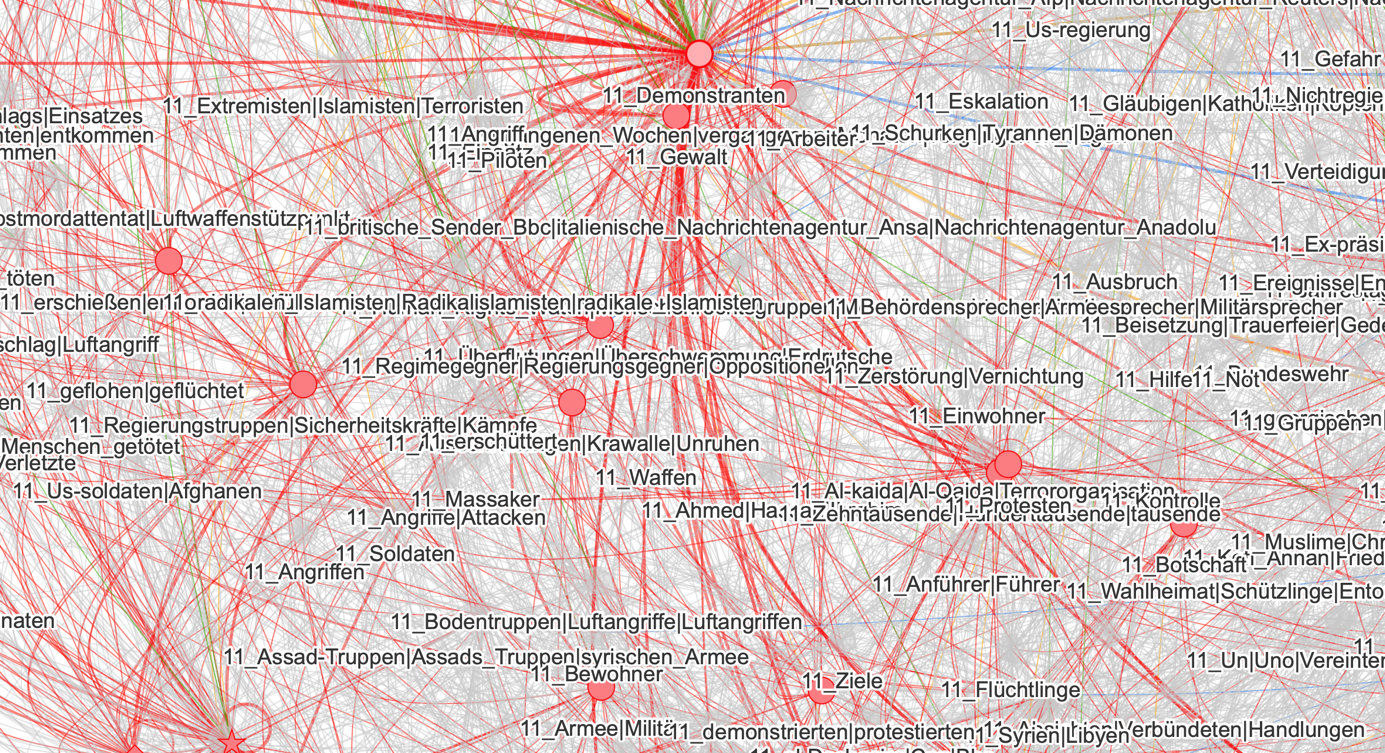
\includegraphics[width=\textwidth]{figures/media/image34.png}
  \caption{\label{fig:islamismus-demonstrationen}Neukonfiguration des Framings von Islamismus bzw. Demonstrationen am Beispiel des FE \cluster{11\_Demonstranten}.}
\end{figure}

Zum Islamismus-Frame sind insbesondere zwei Neukonfigurationen zu nennen: Zum einen schlagen sich die Ereignisse des Arabischen Frühlings deutlich im thematischen Netzwerk-Cluster ‚Krieg \& Islamismus` nieder, sodass nun die auf Demonstrationen bezogenen FE wie \cluster{11\_Protest}, \cluster{11\_Demonstrationen{\breakbar}Kundgebung} oder \cluster{11\_protestieren{\breakbar}demonstrieren}, die zuvor häufig ein eigenes Netzwerk-Cluster bildeten, ein zentraler Teil des thematischen Bereiches ‚Krieg \& Islamismus` werden (\figref{fig:islamismus-demonstrationen}). Zum anderen tritt auch der Bürgerkrieg in Syrien, ebenfalls eine Folge des Arabischen Frühlings, mit FE wie \cluster{11\_syrische\_Opposition{\breakbar}syrische\_Regierung{\breakbar}Präsident\_Assad (politische Akteure Syrienkrieg)}, \cluster{11\_Assads{\breakbar}Präsident\_Baschar\_al-Assad{\breakbar}Regimes (Regime Assad \& Gaddafi)} und \cluster{11\_Assad-Truppen{\breakbar}Assads\_Truppen{\breakbar}syrischen\_Armee (militärische Auseinandersetzungen im Syrienkrieg)} deutlich hervor.

\subsubsection{Fazit}\label{fazit-4}

Im Zeitraum 2011--2013 finden nach einer längeren Phase der Kontinuität größere Umbrüche im Framing einzelner Extremismusvarianten statt. Dabei ist für den Bereich des Rechtsextremismus insbesondere die Wiederkehr eines Framings als gewalttätige, Straftaten begehende Form des Extremismus, wie sie bereits im Zeitraum 1999--2001 vorlag, zu konstatieren. Diese Entwicklung wird durch die Aufdeckung des NSU sowie das Attentat Anders Breiviks ausgelöst und verschiebt den thematischen Fokus der Berichterstattung vom eher abstrakten Bereich eines sozialen, zu bekämpfenden Phänomens in das Netzwerk-Cluster ‚Straftaten \& Juristisches`, was auch eine Replikation der Ergebnisse von Czulo et al. \autocite*{czuloEinflussExtremistischerGewaltereignisse2020} darstellt (siehe \chapref{weitere-arbeiten-zum-extremismusdiskurs-und--begriff}). Die deutliche juristische Prägung ist dabei auch durch den sich über viele Jahre erstreckenden NSU-Prozess sowie das Behördenversagen bei den Ermittlungen zum NSU zu erklären. Auch die juristischen Elemente des Framings der NPD kehren mit dem zweiten NPD-Verbotsverfahren zurück. Der Islamismus-Frame erfährt durch die Ereignisse des Arabischen Frühlings markante Veränderungen. So sind nun Demonstrationen das zentrale, von Bürger*innen ausgeübte Mittel, um gegen die autoritär-islamistischen Regime im Nahen Osten aufzubegehren. Neu zu Tage tritt auch der in Folge des Arabischen Frühlings beginnende Bürgerkrieg in Syrien.

\subsection{Der Zeitraum 2014--2016}\label{der-zeitraum-2014-2016}

\subsubsection{\texorpdfstring{\emph{Corpus-driven} Voranalyse: Thematisch gruppierte Auswahl semantisch äquivalenter Cluster im Vergleich zu den Kern-FE des vorigen Zeitraums}{Corpus-driven Voranalyse: Thematisch gruppierte Auswahl semantisch äquivalenter Cluster im Vergleich zu den Kern-FE des vorigen Zeitraums}}\label{corpus-driven-voranalyse-thematisch-gruppierte-auswahl-semantisch-aequivalenter-cluster-im-vergleich-zu-den-kern-fe-des-vorigen-zeitraums-4}

Die Tabellen \ref{tab:2014_1} und \ref{tab:2014_2} bieten eine Übersicht über die nach Thema gruppierten semantisch äquivalenten Cluster des Zeitraums 2014--2016.

\begin{table}\small
\caption{Thematisch gruppierte Auswahl semantisch äquivalenter Cluster des Zeitraums 2014--2016.}
\label{tab:2014_1}
 \begin{tabularx}{\textwidth}{>{\hsize=0.5\hsize}X >{\hsize=0.5\hsize}X >{\hsize=2.0\hsize}X}
  \lsptoprule
  Extremismus-Variante & Bezug & Frame-Elemente \\
  \midrule
  \multirow{2}{=}{Rechts\-ex\-tre\-mis\-mus} 
  & historisch & \cluster{Holocaust{\breakbar}Nationalsozialismus, Konzentrationslager{\breakbar}Auschwitz-birkenau{\breakbar}Ss, Wehrmacht{\breakbar}Stalin{\breakbar}Roten\_Armee, Auschwitz, Nazis} \\
  & zeit\-ge\-nössisch & \cluster{Neonazis{\breakbar}Rechtsextremisten{\breakbar}Rechtsextreme, Npd, Pegida, Uwe\_Böhnhardt{\breakbar}Uwe\_Mundlos{\breakbar}Böhnhardt, Beate\_Zschäpe{\breakbar}Nsu-prozess, Afd, Frauke\_Petry{\breakbar}Petry{\breakbar}Gauland, Front\_national{\breakbar}Marine\_Le\_Pen{\breakbar}FN, Rassismus{\breakbar}Homophobie{\breakbar}Sexismus, rechtsradikale{\breakbar}rechtsradikalen{\breakbar}rechtsextreme, Heidenau{\breakbar}Freital{\breakbar}Bautzen, Ferguson{\breakbar}Michael\_Brown{\breakbar}Polizeigewalt} \\
  \midrule
  \multirow{2}{=}{Links\-ex\-tre\-mis\-mus} 
  & historisch & \cluster{Ddr} \\
  & zeit\-ge\-nössisch & \cluster{Linke} \\
  \midrule
  \multirow{2}{=}{Politischer Extremismus} 
  & historisch & \cluster{Udssr{\breakbar}Oktoberrevolution{\breakbar}Stalins, Faschisten{\breakbar}Nationalisten{\breakbar}Kommunisten, Weimarer\_Republik{\breakbar}Brd{\breakbar}Ostberlin, Kommunismus{\breakbar}Sozialismus{\breakbar}Diktatur} \\
  & zeit\-ge\-nössisch & \cluster{Antifa{\breakbar}Pegida-Bewegung{\breakbar}Islam-} \\
  \lspbottomrule
 \end{tabularx}
\end{table}

\begin{table}
\caption{Thematisch gruppierte Auswahl semantisch äquivalenter Cluster des Zeitraums 2014--2016.}
\label{tab:2014_2}
 \begin{tabularx}{\textwidth}{>{\hsize=0.5\hsize}X >{\hsize=0.5\hsize}X >{\hsize=2.0\hsize}X}
  \lsptoprule
  Extremismus-Variante & Bezug & Frame-Elemente \\
  \midrule
  {Islamismus} & Nahost\-konflikt & \cluster{Ostjerusalem{\breakbar}Israels\_Armee{\breakbar}radikalislamischen, Hamas, Abbas{\breakbar}Netanjahu{\breakbar}Palästinensern, Gazastreifen{\breakbar}Westjordanland, Jerusalem{\breakbar}Tel\_Aviv{\breakbar}Gaza, israelischen{\breakbar}palästinensische{\breakbar}israelische, Palästinenser{\breakbar}Israelis} \\
  & Syrienkrieg{\slash}Islamischer Staat & \cluster{Baschar\_al-Assad{\breakbar}Machthaber\_Baschar\_al-Assad{\breakbar}Assads, syrischen\_Rebellen{\breakbar}IS-Dschihadisten, Assad, Regime{\breakbar}Assad-regime{\breakbar}militärisch, Al-Nusra-Front{\breakbar}al-Qaida, IS-Miliz{\breakbar}Isis, islamischen\_Staates{\breakbar}iS, kurdische\_Kämpfer{\breakbar}Peschmerga, Kämpfer{\breakbar}Is-kämpfer, Kobane{\breakbar}Mossul{\breakbar}Kobani} \\
  & allgemein & \cluster{Extremisten{\breakbar}Dschihadisten{\breakbar}Islamisten} \\
  \midrule
  varianten\-über\-greifend & Diverses & \cluster{mutmaßlichen\_Terroristen{\breakbar}Abdelhamid\_Abaaoud{\breakbar}Abaaoud} \\
  \lspbottomrule
 \end{tabularx}
\end{table}

\subsubsection{\texorpdfstring{\emph{Corpus-driven} Voranalyse: Cluster mit hoher Cosinus-Distanz im Vergleich zum vorigen Zeitraum}{Corpus-driven Voranalyse: Cluster mit hoher Cosinus-Distanz im Vergleich zum vorigen Zeitraum}}\label{corpus-driven-voranalyse-cluster-mit-hoher-cosinus-distanz-im-vergleich-zum-vorigen-zeitraum-4}

Unter den Ergebnissen (siehe \tabref{tab:cluster-high-cosine-distance-2014}) dieser Voranalyse zeichnen sich als für den Extremismusdiskurs besonders relevant das Erstarken des \cluster{14\_iS}, die sogenannte \cluster{14\_Flüchtlingskrise}, die Kölner \cluster{14\_Silvesternacht} sowie die Ereignisse um die Tötung Michael Browns durch Polizeigewalt in den USA ab.

\begin{table}[t]\small
\caption{Cluster mit hoher Cosinus-Distanz im Vergleich zum vorigen Zeitraum.}
\label{tab:cluster-high-cosine-distance-2014}
\begin{tabularx}{\textwidth}{X r}
\lsptoprule
Cluster & Cos.-Dist. \\
\midrule
\cluster{iS} & 0.93 \\
\cluster{Flüchtlingskrise} & 0.49 \\
\cluster{Krim} & 0.45 \\
\cluster{Ferguson{\breakbar}Michael\_Brown{\breakbar}Polizeigewalt} & 0.43 \\
\cluster{Silvesternacht} & 0.41 \\
\cluster{Minsk} & 0.4 \\
\cluster{Frauke\_Petry{\breakbar}Petry{\breakbar}Gauland} & 0.39 \\
\cluster{Trump{\breakbar}Donald\_Trump} & 0.36 \\
\cluster{Edathy{\breakbar}Hartmann{\breakbar}Ziercke} & 0.36 \\
\cluster{Westafrika} & 0.34 \\
\cluster{Sierra\_Leone{\breakbar}Liberia{\breakbar}Guinea} & 0.31 \\
\cluster{Mariupol{\breakbar}Slowjansk{\breakbar}Luhansk} & 0.31 \\
\cluster{Clinton{\breakbar}Hillary\_Clinton} & 0.31 \\
\cluster{Bundesaußenminister\_Frank-walter\_Steinmeier{\breakbar}Außenminister\_Frank-walter\_Steinmeier} & 0.3 \\
\cluster{Putschversuch{\breakbar}Putsch} & 0.27 \\
\cluster{Heidenau{\breakbar}Freital{\breakbar}Bautzen} & 0.27 \\
\cluster{Flüchtlingspolitik} & 0.27 \\
\cluster{Obergrenze} & 0.23 \\
\cluster{Kobane{\breakbar}Mossul{\breakbar}Kobani} & 0.23 \\
\cluster{Schlepper{\breakbar}Schleuser} & 0.21 \\
\lspbottomrule
\end{tabularx}
\end{table}

\subsubsection{Rechts- und Linksextremismus}\label{rechts--und-linksextremismus-5}

Wie schon zuvor lässt sich aus dem Gesamt-Frame zum politischen Extremismus ein historischer Anteil abgrenzen, der wiederum unterschiedliche Teil-Frames enthält. Darunter ein Frame zur NS-Zeit um die FE \cluster{14\_Holocaust{\breakbar}Nationalsozialismus}, \cluster{14\_Konzentrationslager{\breakbar}Konzentrationslagern{\breakbar}Auschwitz-birkenau}, \cluster{14\_Wehrmacht{\breakbar}Stalin{\breakbar}Roten\_Armee (Akteure NS-Zeit)}, \cluster{14\_Auschwitz} und \cluster{14\_Nazis}; ein Frame zum Totalitarismus bzw. dem 20 Jahrhundert inklusive der Zeit des Kalten Krieges (\cluster{14\_}Udssr{\breakbar}\cluster{Oktoberrevolution{\breakbar}Stalins} (20. Jhdt), \cluster{14\_}Faschisten{\breakbar}\cluster{Nationalisten{\breakbar}Kommunisten} (Anhänger Totalitarismus), \cluster{14\_}Weimarer\cluster{\_Republik{\breakbar}Brd{\breakbar}Ostberlin} (Deutschland 20. Jhdt), \cluster{14\_Kommunismus{\breakbar}Sozialismus{\breakbar}Diktatur (Totalitarismus)}) und letztlich das ausschließlich auf die DDR bezogene FE \cluster{14\_Ddr}. Wie schon in den vorigen Zeiträumen ist das Framing hier insbesondere auf den thematischen Bereich ‚Staat, FdGO \& Gesellschaft` konzentriert, der die Bedrohung dieser Ereignisse für \cluster{14\_Freiheit} und \cluster{14\_Demokratie} deutlich macht und das \cluster{14\_Gedenken} an sie herausstellt. Dabei sind die Ereignisse bzw. Menschen, derer gedacht wird (\cluster{14\_Toten{\breakbar}Todesopfer}, \cluster{14\_Opfer}, \cluster{14\_getöteten{\breakbar}ermordeten{\breakbar}toten}), häufig in einem in diesem Zeitraum neu entstehenden Teil-Frame zu finden, der ‚Tod \& Attentate` thematisiert.\largerpage

Deutlichere Veränderungen, die zu einem großen Teil auf die Fluchtbewegungen der Jahre 2015 und 2016 zurückgehen, finden sich im zeitgenössischen Teil des Rechtsextremismus-Frame. Hier ist zum einen die PEGIDA-Bewegung zu nennen, die -- wie zuvor andere Bewegungen des politischen Extremismus in Deutschland -- insbesondere durch das Agieren im Rahmen von Demonstrationen geframet wird (u.\,a. \cluster{14\_demonstrieren}, \cluster{14\_Aufruf{\breakbar}Appell}, \cluster{14\_Straße}). Durch die Vernetzung mit rechten politischen Akteuren (\cluster{14\_Frauke\_Petry{\breakbar}Petry{\breakbar}Gauland}, \cluster{14\_Npd}) sowie Charakteristika des Rechtsextremismus (\cluster{14\_rechtsradikale{\breakbar}rechtsradikalen{\breakbar}rechtsextreme}, \cluster{14\_Fremdenfeindlichkeit{\breakbar}Intoleranz{\breakbar}Antisemitismus}) wird der rechtsextreme Charakter der Bewegung deutlich. Ein ähnliches Framing, das noch etwas stärker FE zum thematischen Feld des Demonstrierens bindet, zeigt auch das FE \cluster{14\_Antifa{\breakbar}Pegida-Bewegung{\breakbar}Islam}-, das eine breitere Sammlung an Wörtern zur PEGIDA-Bewegung sowie den Protesten und Gegenprotesten enthält (u.\,a. \emph{Aufmärsche}, \emph{linken\_Szene}, \emph{Mob}, \emph{Protestbewegung}, \emph{Pegida-Bewegung}). Mit der Kölner \cluster{14\_Silvesternacht} und der politisch-medial breit geführten Diskussion zu einer \cluster{14\_Obergrenze} hat die \emph{corpus-driven} Voranalyse (\chapref{corpus-driven-voranalyse-cluster-mit-hoher-cosinus-distanz-im-vergleich-zum-vorigen-zeitraum-4}) außerdem zwei Schlagwörter zu Tage gefördert, die für zwei zentrale Diskursereignisse des Zeitraums stehen. Während sich die Diskussion um eine Migrationsobergrenze zwischen den thematischen Frame-Anteilen ‚Flucht \& Migration` sowie ‚Politik` entspannt, wird die Kölner Silvesternacht als juristisch relevantes Ereignis geframet. Dabei changieren die angeschlossenen FE (siehe \figref{fig:silvesternacht-straftaten}) zwischen schweren Straftaten (\cluster{14\_Gewalttaten{\breakbar}Morde{\breakbar}Übergriffe}, \cluster{14\_Straftaten}, \cluster{14\_Täter}) und eher verharmlosenden Begriffen wie \cluster{14\_Vorkommnisse{\breakbar}Verfehlungen{\breakbar}Missstände}.

\begin{figure}[t]
  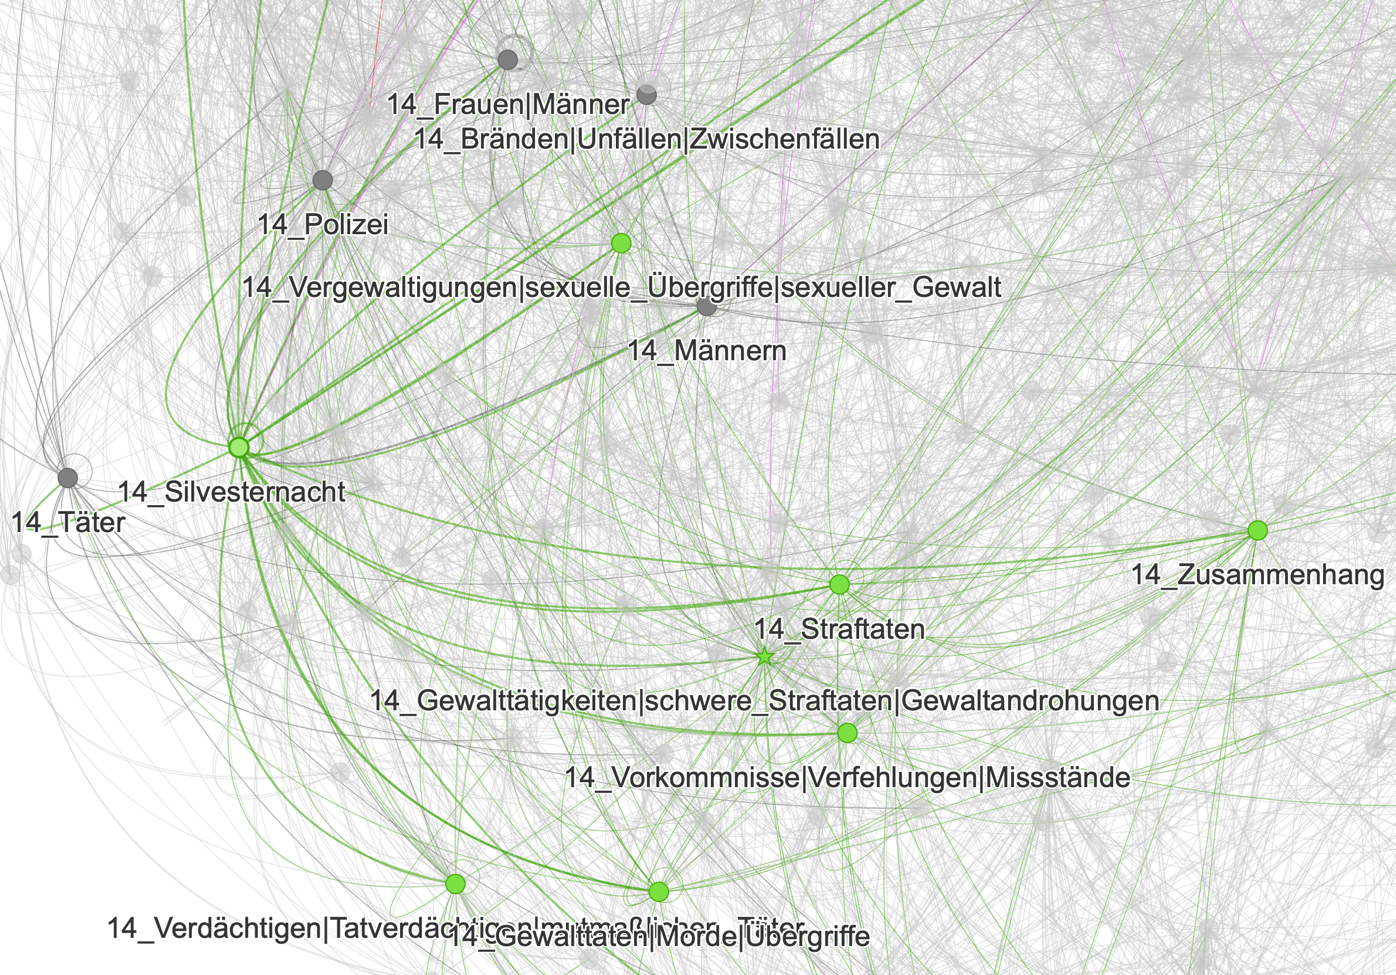
\includegraphics[width=\textwidth]{figures/media/image35.png}
  \caption{\label{fig:silvesternacht-straftaten}Teil der Vernetzung des FE \cluster{14\_Silvesternacht} im Bereich ‚Straftaten \& Juristisches`.}
\end{figure}

Mit dem FE \cluster{14\_Heidenau{\breakbar}Freital{\breakbar}Bautzen} erhalten außerdem einzelne ostdeutsche Orte, an denen rechte Attentate auf Asylunterkünfte verübt wurden, Einzug in den Varianten-Frame. Die verlinkten FE geben dabei Aufschluss über die Art der Anschläge -- aus dem neu entstehenden Migrations-Teil-Frame sind dies etwa \cluster{14\_Flüchtlingsunterkünfte{\breakbar}Flüchtlingsheime{\breakbar}Unterkünfte}, \cluster{14\_Notunterkunft{\breakbar}Erstaufnahmeeinrichtung{\breakbar}Unterkunft} sowie aus dem Cluster um Tod \& Attentate u.\,a. \cluster{14\_Bränden{\breakbar}Unfällen{\breakbar}Zwischenfällen} und \cluster{14\_Brand}. Auch der thematische Bereich ‚Demonstrationen \& politischer Extremismus` leistet eine weitere epistemische Spezifizierung durch die FE \cluster{14\_Ausschreitungen} und \cluster{14\_rechtsradikale{\breakbar}rechtsradikalen{\breakbar}rechtsextreme}. Am angeschlossenen Cluster \cluster{14\_Kanzlerin{\breakbar}Merkel{\breakbar}Angela\_Merkel} lassen sich außerdem Versuche der politischen Auseinandersetzung mit diesen Anschlägen sowie der von rechten Teilen der Bevölkerung gegen die damalige Bundeskanzlerin Merkel gerichtete Hass nachvollziehen (siehe Belege K23--K25 in \tabref{tab:K23-K25}).

\begin{table}
  \caption{Konkordanzen zur Kollokation der Cluster \cluster{14\_Heidenau{\breakbar}Freital{\breakbar}Bautzen} und \cluster{14\_Kanzlerin{\breakbar}Merkel{\breakbar}Angela\_Merkel}.}
  \label{tab:K23-K25}
K23 welt\_3334259
\begin{tabularx}{\textwidth}{QQQ}
\toprule
D-Flüchtlinge-Sachsen-Polizei-Einwanderung-Gewalt-Regierung Merkel nennt Ausschreitungen gegen Flüchtlinge beschämend & {[}14\_Kanzlerin{\breakbar}Merkel{\breakbar}Angela\_Merkel: \emph{\textbf{Kanzlerin}}{]}\newline
\textbf{kritisiert alkoholisierte} \textbf{Schreihälse in}\newline
{[}Heidenau{\breakbar}Freital{\breakbar}Bautzen: \emph{\textbf{Heidenau}}{]} & Bundeskanzlerin\_Angela\_Merkel Cdu hat die wiederholten\_Ausschreitungen an dem Asylbewerberheim im sächsischen\_Heidenau als beschämend kritisiert die Bundeskanzlerin \\
\bottomrule
\end{tabularx}
\bigskip \newline
K24 spiegel\_3335667
\begin{tabularx}{\textwidth}{QQQ}
\toprule
schon leben dass es irgendwann Tote gibt ist angesichts der Gewaltbereitschaft mancher Kreise nicht ausgeschlossen & {[}14\_Kanzlerin{\breakbar}Merkel{\breakbar}Angela\_Merkel: \emph{\textbf{Merkel}}{]}\newline
\textbf{muss in}\newline
{[}Heidenau{\breakbar}Freital{\breakbar}Bautzen: \emph{\textbf{Heidenau}}{]} & spüren dass die Frage wie die Republik mit den Hunderttausenden\_Flüchtlingen umgehen soll mancherorts das Zeug \\
\bottomrule
\end{tabularx}
\bigskip \newline
K25 taz\_3670491
\begin{tabularx}{\textwidth}{QQQ}
\toprule
Bahnhöfen sah man erschöpfte Familien auf dem Schoß abgerissene Kinder fünf Tage zuvor hatten in & {[}Heidenau{\breakbar}Freital{\breakbar}Bautzen: \emph{\textbf{Heidenau}}{]}\newline
\textbf{Fremdenfeinde die}\newline
{[}14\_Kanzlerin{\breakbar}Merkel{\breakbar}Angela\_Merkel: \emph{\textbf{Kanzlerin}}{]} & als Volksverräterin angepöbelt tags\_darauf waren in einem abgestellten Kühllaster auf der österreichischen Autobahn die verwesten\_Leichen \\
\bottomrule
\end{tabularx}
\end{table}

Auch die AfD ist nach ihrem Wandel von einer vordergründig auf wirtschaftliche Themen ausgerichteten Partei zu einer asylkritischen Rechtsaußen-Partei mit den Clustern \cluster{14\_AfD} und \cluster{14\_Frauke\_Petry{\breakbar}Petry{\breakbar}Gauland} im Frame repräsentiert. Neben Frame-Relationen im Bereich der Innenpolitik weist die Partei auch eine starke Verankerung im Bereich ‚Demonstrationen \& politischer Extremismus` auf. Als Partei des äußeren rechten Spektrums wird sie insbesondere durch Anbindungen an rechtxextreme Attribuierungen wie \cluster{14\_Fremdenfeindlichkeit{\breakbar}Intoleranz{\breakbar}Antisemitismus} und \cluster{14\_rechtsradikale{\breakbar}rechtsradikalen{\breakbar}rechtsextreme} epistemisch konturiert. Auch die in Beziehung stehenden politischen Parteien \cluster{14\_Npd}, \cluster{14\_Front\_national{\breakbar}Marine\_Le\_Pen{\breakbar}FN}, die zu Parteien wie \cluster{14\_Union} oder \cluster{14\_Grüne} keine Verbindungen aufweisen, geben Hinweise auf die Stellung im Parteiensystem.

Einen weiteren neuen Akzent markiert in diesem Zeitraum das FE \cluster{14\_Ferguson{\breakbar}Michael\_Brown{\breakbar}Polizeigewalt}, das die Ereignisse um die Tötung Michael Browns durch einen Polizisten im US-amerikanischen Ferguson und die sich anschließenden Debatten und Proteste gegen rassistische Polizeigewalt abbildet. Sichtbar wird dies in FE wie \cluster{14\_Polizei}, \cluster{14\_Schwarze{\breakbar}Schwarzen{\breakbar}Afroamerikaner}, \cluster{14\_Ausschreitungen} oder \cluster{14\_Rassismus{\breakbar}Homophobie{\breakbar}Sexismus}.

\subsubsection{Islamismus}\label{islamismus-5}

Der Islamismus-Frame ist in diesem Zeitraum besonders durch das Erstarken des Islamischen Staates (IS) sowie den damit in Zusammenhang stehenden Syrienkrieg geprägt, was sich in einer Vielzahl von FE im Bereich ‚Krieg \& Islamismus` niederschlägt. Dabei werden sowohl (para\mbox{-})militärische Akteure wie die Cluster \cluster{14\_Kämpfer{\breakbar}Is-kämpfer}, \cluster{14\_syrischen\_Rebellen{\breakbar}syrische\_Rebellen{\breakbar}IS}- und \cluster{14\_kurdische\_Kämpfer{\breakbar}irakischen\_Armee{\breakbar}Pschmerga}; Orte (\cluster{14\_Kobane{\breakbar}Mossul{\breakbar}Kobani}) als auch Terrororganisationen (\cluster{14\_iS}, \cluster{14\_Al-Nusra-Front{\breakbar}Nusra-Front{\breakbar}al-Qaida}) als Teil des Islamismus-Frames offenbar. Die angeschlossenen FE außerhalb des Bereiches ‚Krieg \& Islamismus`framen den IS zu einem großen Teil in seiner Eigenschaft als Organisation, bei der Fragen der Unterstützung bzw. Mitgliedschaft virulent werden: u.\,a. \cluster{14\_Reihen{\breakbar}eigenen\_Reihen}, \cluster{14\_Mitglied}, \cluster{14\_Gruppen{\breakbar}Gruppierungen{\breakbar}Aktionen}, \cluster{14\_Netzwerke{\breakbar}Aktivitäten{\breakbar}Dienste}, \cluster{14\_Gruppe}, \cluster{14\_Anhänger}. Dies hängt auch damit zusammen, dass -- wie bereits zuvor gezeigt -- Fragen der Anhängerschaft von extremistischen Gruppen im Extremismusdiskurs von höchster Bedeutung sind. Dies liegt bei Terrororganisationen wie dem IS neben der gesellschaftlich-ethischen Bedeutung dieses Aspektes auch an der Relevanz für Fragen der inneren Sicherheit und der juristischen Bedeutung, die der Straftatbestand der Mitgliedschaft in einer ausländischen terroristischen Vereinigung hat. Die Konkordanzen K26--K28 in \tabref{tab:K26-K28} illustrieren dies näher.

\begin{table}[t]
  \caption{Konkordanzen zur Kollokation der Cluster \cluster{14\_Mitglied} und \cluster{14\_iS}.}
  \label{tab:K26-K28}
K26 welt\_3668970
\begin{tabularx}{\textwidth}{QQQ}
\toprule
erste islamistische Selbstmordanschlag in Deutschland die Bundesanwaltschaft\_prüft den Verdacht dass der 27-jährige Täter aus Syrien & {[}14\_Mitglied: \textbf{Mitglied}{]}\newline
\textbf{in der Terrormiliz\_islamischer\_Staat}\newline
{[}14\_iS: \textbf{iS}{]} & war wie die Bild unter\_Berufung auf ein psychologisches Fachgutachten berichtet schätzte ein Therapeut aus Lindau \\
\bottomrule
\end{tabularx}
\bigskip \newline
K27 spiegel\_3441101
\begin{tabularx}{\textwidth}{QQQ}
\toprule
zu benennen Ayoub\_B lt100 Jahre\_alt und Ebrahim\_H\_B lt100 Jahre waren nach Überzeugung des Senats beide & {[}14\_Mitglied: \textbf{Mitglied}{]}\newline
\textbf{des}\newline
{[}14\_iS: \textbf{iS}{]} & dass sie Ende Mai 2014 nach\_Syrien\_gereist sind um den Islam zu studieren oder humanitäre\_Hilfe zu \\
\bottomrule
\end{tabularx}
\bigskip \newline
K28 spiegel\_3130133
\begin{tabularx}{\textwidth}{QQQ}
\toprule
hatte der Mann aus Mülheim an der Ruhr ist dringend\_verdächtig sich im vergangenen Sommer als & {[}14\_Mitglied: \textbf{Mitglied}{]}\newline
\textbf{der Terrororganisation\_islamischer\_Staat}\newline
{[}14\_iS: \textbf{iS}{]} & mehrfach an Kampfhandlungen in Syrien beteiligt zu haben er war über Syrien in das Bürgerkriegsland \\
\bottomrule
\end{tabularx}
\end{table}

Im Cluster \cluster{14\_mutmaßlichen\_Terroristen{\breakbar}Abdelhamid\_Abaaoud{\breakbar}Abaaoud (Attentate in Europa)} sind darüber hinaus Wörter zu diversen in Europa verübten Attentaten vereint. Darunter der Anschlag auf dem \emph{Berliner\_Breitscheidplatz} durch \emph{Anis\_Amri}; die Pariser Anschläge von 2015, verübt durch die IS-Mitglieder \emph{Abdelhamid\_Abaaoud}, \emph{Amedy\_Coulibaly} und \emph{Salah\_Abdeslam} und unter Beteiligung von \emph{Najim\_Laachraoui}, der darüber hinaus auch einen Bombenanschlag auf den Brüsseler Flughafen im Jahr 2016 beging; das rechtsextremistisch motivierte Attentat auf Henriette Reker durch \emph{Frank\_S}; das mutmaßlich von \emph{Dschaber al-Bakr} geplante Attentat auf den Berliner Flughafen Tegel; die Anschläge durch \emph{Anders Breivik}, das \emph{NSU-Trio} und weitere. Das Cluster weist eine starke Vernetzung im Frame-Anteil ‚Straftaten \& Juristisches` auf, die durch Ermittlungen und mithin in der Berichterstattung verwendete Ausdrücke der epistemischen Unsicherheit (\cluster{14\_Hinweise}, \cluster{14\_angebliche{\breakbar}angeblichen{\breakbar}vermeintlichen}, \cluster{14\_Bericht\_zufolge}, \cluster{14\_offensichtlich{\breakbar}offenkundig{\breakbar}anscheinend}) geprägt ist. Wissenselemente, die die Taten selbst näher spezifizieren, sind in den Clustern ‚Krieg \& Islamismus` (\cluster{14\_Geiseln}, \cluster{14\_Anschlägen}, \cluster{14\_Anschlag{\breakbar}Attentat{\breakbar}Terroranschlag}) sowie ‚Tod \& Attentate` (\cluster{14\_tötete{\breakbar}erschoss{\breakbar}erschießt}, \cluster{14\_Lastwagen{\breakbar}Lkw}, \cluster{14\_Attacke}) zu finden.

\subsubsection{Fazit}\label{fazit-5}

Im Zeitraum 2014--2016 verändert sich das Framing von Extremismusvarianten erneut deutlich. Bereits in der Makrostruktur des Clusters kristallisieren sich durch die Fluchtbewegungen der Jahre 2015 und 2016 sowie eine Vielzahl von Anschlägen in Europa die Themenfelder ‚Flucht \& Migration` sowie ‚Tod \& Attentate` heraus. Beide Themen stehen in einem inhaltlichen Zusammenhang mit dem Erstarken des IS, das sich im Cluster ‚Krieg \& Islamismus` in einer Vielzahl von FE widerspiegelt. Im Bereich des Rechtsextremismus treten vor diesem Hintergrund mit PEGIDA, der AfD sowie den Brandanschlägen auf Asylunterkünfte neue Akteure und Formen extremistischer Gewalt zu Tage.

\subsection{Der Zeitraum 2017--2019}\label{der-zeitraum-2017-2019}

\subsubsection{\texorpdfstring{\emph{Corpus-driven} Voranalyse: Thematisch gruppierte Auswahl semantisch äquivalenter Cluster im Vergleich zu den Kern-FE des vorigen Zeitraums}{Corpus-driven Voranalyse: Thematisch gruppierte Auswahl semantisch äquivalenter Cluster im Vergleich zu den Kern-FE des vorigen Zeitraums}}\label{corpus-driven-voranalyse-thematisch-gruppierte-auswahl-semantisch-aequivalenter-cluster-im-vergleich-zu-den-kern-fe-des-vorigen-zeitraums-5}

Einen Überblick über die thematisch gruppierte Auswahl semantisch äquivalenter Cluster des Zeitraums 2017--2019 gibt \tabref{tab:2017}.

\begin{table}[t]\small
\caption{Thematisch gruppierte Auswahl semantisch äquivalenter Cluster des Zeitraums 2017--2019.}
\label{tab:2017}
 \begin{tabularx}{\textwidth}{>{\hsize=0.5\hsize}X >{\hsize=0.5\hsize}X >{\hsize=2.0\hsize}X}
  \lsptoprule
  Extremismus-Variante & Bezug & Frame-Elemente \\
  \midrule
  \multirow{2}{=}{Rechts\-ex\-tre\-mis\-mus} 
  & historisch & \cluster{Nationalsozialisten{\breakbar}Holocaust{\breakbar}Nationalsozialismus, Judenverfolgung{\breakbar}Vernichtungslager{\breakbar}Konzentrationslager} \\
  & zeit\-ge\-nössisch & \cluster{Rechtsextremisten{\breakbar}Rechtsextreme{\breakbar}Neonazis, rechtsradikalen{\breakbar}rechtsextremen{\breakbar}rechtsextreme, Gauland{\breakbar}Meuthen{\breakbar}Weidel, Uwe\_Böhnhardt{\breakbar}Böhnhardt{\breakbar}Uwe\_Mundlos, André\_E{\breakbar}Nsu-prozess{\breakbar}Beate\_Zschäpe, Antisemitismus{\breakbar}Rassismus} \\
  \midrule
  \multirow{2}{=}{Links\-ex\-tre\-mis\-mus} 
  & historisch & - \\
  & zeit\-ge\-nössisch & - \\
  \midrule
  \multirow{2}{=}{Politischer Extremismus} 
  & historisch & \cluster{Ddr{\breakbar}Weimarer\_Republik{\breakbar}Sowjetunion, Kommunismus{\breakbar}Sozialismus{\breakbar}Diktatur, Bolschewiki{\breakbar}Kommunisten{\breakbar}kommunistischen} \\
  & zeit\-ge\-nössisch & \cluster{Linkspartei{\breakbar}Afd{\breakbar}Linken, Rechtsradikalen{\breakbar}Rechtsradikale{\breakbar}Rechtsextremen} \\
  \midrule
  {Islamismus} & Nahost\-konflikt & \cluster{Ostjerusalem{\breakbar}Ramallah{\breakbar}Hebron, Gazastreifen{\breakbar}Westjordanland, Hamas, Palästinensern{\breakbar}Israelis} \\
  & Syrienkrieg{\slash}Islamischer Staat & \cluster{Regierungstruppen{\breakbar}Provinz\_Idlib{\breakbar}syrischen\_Armee, Idlib{\breakbar}Afrin{\breakbar}Damaskus, Dschihadisten, Terrormiliz{\breakbar}Terrormiliz\_iS{\breakbar}Terrormiliz\_islamischer\_Staat, Pkk{\breakbar}Terrororganisation{\breakbar}Gülen-bewegung, iS, kurdische{\breakbar}kurdischen{\breakbar}syrische} \\
  & Weiteres & \cluster{Huthi-Rebellen{\breakbar}Huthis{\breakbar}Hisbollah, Amri} \\
  \midrule
  varianten\-über\-greifend & Diverses & \cluster{Rechtsextremismus{\breakbar}Islamismus{\breakbar}Extremismus, rechtsextremistischen{\breakbar}gewaltbereiten{\breakbar}militanten, El\_Paso{\breakbar}Christchurch{\breakbar}Pittsburgh} \\
  \lspbottomrule
 \end{tabularx}
\end{table}

\subsubsection{\texorpdfstring{\emph{Corpus-driven} Voranalyse: Cluster mit hoher Cosinus-Distanz im Vergleich zum vorigen Zeitraum}{Corpus-driven Voranalyse: Cluster mit hoher Cosinus-Distanz im Vergleich zum vorigen Zeitraum}}\label{corpus-driven-voranalyse-cluster-mit-hoher-cosinus-distanz-im-vergleich-zum-vorigen-zeitraum-5}

In diesem Zeitraum prägen außenpolitische Veränderungen, darunter insbesondere die Wahl Donald Trumps zum US-Präsidenten und auch der Brexit, die semantischen Verschiebungen im Vektorraum (siehe \tabref{tab:cluster-high-cosine-distance-2017}). Des Weiteren spiegeln sich als extremismusbezogene Ereignisse rechte Attentate in den USA (\cluster{17\_El\_Paso{\breakbar}Christchruch{\breakbar}Pittsburgh}) und der \emph{G-20-Gipfel} in Hamburg wider.

\begin{table}[t]\small
\caption{Cluster mit hoher Cosinus-Distanz im Vergleich zum vorigen Zeitraum.}
\label{tab:cluster-high-cosine-distance-2017}
\begin{tabularx}{\textwidth}{X r}
\lsptoprule
Cluster & Cos.-Dist. \\
\midrule
\cluster{Dezember\_2016} & 0.62 \\
\cluster{Us-präsident\_Donald\_Trump{\breakbar}Us-präsident\_Trump{\breakbar}Präsident\_Donald\_Trump} & 0.51 \\
\cluster{Puigdemont{\breakbar}Carles\_Puigdemont} & 0.44 \\
\cluster{Mueller{\breakbar}Flynn{\breakbar}Comey} & 0.39 \\
\cluster{G20-gipfel{\breakbar}G-20-Gipfel{\breakbar}beim\_G20-gipfel} & 0.37 \\
\cluster{El\_Paso{\breakbar}Christchurch{\breakbar}Pittsburgh} & 0.36 \\
\cluster{Macron} & 0.35 \\
\cluster{Bolton{\breakbar}Tillerson{\breakbar}Pompeo} & 0.28 \\
\cluster{Kim} & 0.23 \\
\cluster{May{\breakbar}Theresa\_May{\breakbar}Premierministerin\_Theresa\_May} & 0.22 \\
\cluster{Premierministerin\_May{\breakbar}Eu-ratspräsident\_Donald\_Tusk{\breakbar}Eu-kommissionspräsident\_Jean-claude\_Juncker} & 0.21 \\
\cluster{de\_Maizière{\breakbar}De\_Maizière{\breakbar}Pistorius} & 0.2 \\
\cluster{Einzelhaft{\breakbar}Hausarrest{\breakbar}türkischer\_Haft} & 0.2 \\
\cluster{Dekret{\breakbar}Einreiseverbot} & 0.19 \\
\cluster{Wahlbeeinflussung{\breakbar}des\_Trump-Teams{\breakbar}russische\_Hacker} & 0.19 \\
\cluster{Bogotá{\breakbar}Nairobi{\breakbar}Lagos} & 0.17 \\
\cluster{Us-justiz{\breakbar}Missbrauchsvorwürfe{\breakbar}wegen\_sexueller\_Belästigung} & 0.17 \\
\cluster{Trumps{\breakbar}Donald\_Trumps} & 0.17 \\
\cluster{Alan\_Kurdi{\breakbar}Open\_Arms{\breakbar}Aquarius} & 0.17 \\
\cluster{Backstop{\breakbar}Eu-austritt\_Großbritanniens{\breakbar}Austrittsvertrag} & 0.17 \\
\lspbottomrule
\end{tabularx}
\end{table}

\subsubsection{Rechts- und Linksextremismus}\label{rechts--und-linksextremismus-6}

Der Rechtsextremismus-Frame dieses Zeitraumes ist eher durch Kontinuitäten als Brüche im Framing gekennzeichnet. Nach wie vor macht der NSU-Prozess mit den FE \cluster{17\_Uwe\_Böhnhardt{\breakbar}Böhnhardt{\breakbar}Uwe\_Mundlos} und \cluster{17\_André\_E{\breakbar}Nsu-prozess{\breakbar}Beate\_Zschäpe} einen stark juristisch geprägten Anteil aus. Es finden sich nur einzelne Verbindungen in andere thematische Bereiche, so in das Netzwerk-Cluster ‚Tod \& Attentate` (\cluster{17\_erschossen{\breakbar}ermordet}, \cluster{17\_verstorbenen{\breakbar}gestorbenen{\breakbar}Todestag}, \cluster{17\_Opfer{\breakbar}Opfern}), das den NSU-Komplex stärker in Hinblick auf die ermordeten Menschen sowie das Gedenken an sie perspektiviert, und in den Bereich ‚Politischer Extremismus \& Demonstrationen`, der Organisationsaspekte (\cluster{17\_Netzwerk}) sowie den gewalttätig-extremistischen Charakter (\cluster{17\_rechtsextremistischen{\breakbar}gewaltbereiten{\breakbar}militanten}) des NSU einbindet.

Das FE \cluster{17\_Gauland{\breakbar}Meuthen{\breakbar}Weidel (NPD{\slash}AfD-Politiker*innen{\slash}Sahra Wagenknecht)} ist zum einen Teil des Clusters ‚Politik`, zum anderen klar als rechtsextremistisch geframet. Hierzu trägt neben FE aus dem Feld ‚Demonstrationen \& politischer Extremismus` (\cluster{17\_rechtsradikalen{\breakbar}rechtsextremen{\breakbar}rechtsextreme {[}attributive Charakteristika Rechtsextremismus{]}}, \cluster{17\_Rechtsextremismus{\breakbar}Islamismus{\breakbar}Extremismus {[}Extremismusformen{\slash}Radikalisierung{\slash}Fremdenfeindlichkeit{]})} auch das FE \cluster{17\_Verfassungsschutz} bei, das insbesondere für die Beobachtung des ‚Flügels` um Björn Höcke durch den Verfassungsschutz steht.

Die FE \cluster{17\_Rechtsextremisten{\breakbar}Rechtsextreme{\breakbar}Neonazis} und \cluster{17\_rechtsradikalen{\breakbar}rechtsextremen{\breakbar}rechtsextreme (attributive Charakteristika Rechtsextremismus)} versprachlichen Rechtsextremismus zu einem großen Teil explizit. Die an sie angeschlossenen FE sind häufig Objekt der Zuschreibung, rechtsextremistisch zu sein bzw. dem Rechtsextremismus nahe zu stehen. Hierunter fallen einerseits Parteien und Politiker wie in den FE \cluster{17\_Orbán{\breakbar}Viktor\_Orbán{\breakbar}Ungarns}, \cluster{17\_Pd{\breakbar}Podemos{\breakbar}PSOE} oder \cluster{17\_Le\_Pen{\breakbar}Marine\_Le\_Pen{\breakbar}Emmanuel\_Macron}, aber auch die Bundeswehr (\cluster{17\_Bundeswehr}, \cluster{17\_Truppe}), die in Bezug auf rechtextreme Vorfälle zum Gegenstand des medialen Extremismusdiskurses wird (siehe Belege K29--K31 in \tabref{tab:K29-K31}).

\begin{table}[h]\small
  \caption{Konkordanzen zur Kollokation der Cluster \cluster{17\_rechtsradikalen{\breakbar}rechtsextremen{\breakbar}rechtsextreme} und \cluster{17\_Truppe}.}
  \label{tab:K29-K31}
K29 spiegel\_4166845
\begin{tabularx}{\textwidth}{QQQ}
\toprule
sich durch Fehler als Ministerin geschwächt in der Bundeswehr ist sie umstritten seit sie der & {[}17\_Truppe: \textbf{Truppe}{]}\newline
\textbf{nach einzelnen}\newline
{[}17\_rechtsradikalen{\breakbar}rechtsextremen{\breakbar}rechtsextreme: \textbf{rechtsradikalen}{]} & Vorfällen ein Haltungsproblem\_attestiert hat in der Folge kam es zu einem regelrechten Aufstand in der \\
\bottomrule
\end{tabularx}
\bigskip \newline
K30 spiegel\_4272324
\begin{tabularx}{\textwidth}{QQQ}
\toprule
nach einer\_Kleinen\_Anfrage der Grünen-abgeordneten\_Irene\_Mihalic und Konstantin von Notz beide wollten vor\_allem wissen ob sich möglicherweise & {[}17\_rechtsradikalen{\breakbar}rechtsextremen{\breakbar}rechtsextreme: \textbf{rechtsextreme}{]}\newline
\textbf{Soldaten bei der}\newline
{[}17\_Truppe: \textbf{Truppe}{]} & mit Waffen und Munition eingedeckt haben könnten die Antwort ist teilweise kurios so wurden die \\
\bottomrule
\end{tabularx}
\bigskip \newline
K31 welt\_3932906
\begin{tabularx}{\textwidth}{QQQ}
\toprule
konkrete\_Hinweise seien nicht ernst\_genommen worden sagte der Generalinspekteur dem Nachrichtenmagazin stattdessen habe sich in der & {[}17\_Truppe: \textbf{Truppe}{]}\newline
\textbf{gegenüber}\newline
{[}17\_rechtsradikalen{\breakbar}rechtsextremen{\breakbar}rechtsextreme: \textbf{rechtsextremen}{]} & Soldaten ein Muster des Wegsehens etabliert schon 2014 habe es interne Warnsignale gegeben sagte Wieker \\
\bottomrule
\end{tabularx}
\end{table}

Auch das FE \cluster{17\_El\_Paso{\breakbar}Christchurch{\breakbar}Pittsburgh} findet sich unter den verlinkten FE. Es vereint die rechtsextrem motivierten Anschläge von El Paso, Christchurch, Pittsburgh und Charlottesville sowie einen Amoklauf in Parkland und ein islamistisches Attentat in Manchester. Es ist seinerseits im Bereich ‚Demonstrationen \& politischer Extremismus` vernetzt, der die Ereignisse als extremistisch framet. Zudem finden sich Bezüge in den thematischen Bereich ‚Tod \& Anschläge` (u.\,a. \cluster{17\_Attentäter}, \cluster{17\_Todesopfer{\breakbar}Todesopfern{\breakbar}Verletzten}) und Politik (u.\,a. \cluster{17\_Bürgermeister{\breakbar}Oberbürgermeister}, \cluster{17\_Reaktion}, \cluster{17\_Trump{\breakbar}Donald\_Trump{\breakbar}Us-präsident}).

Der Bereich des Linksextremismus ist in diesem Zeitraum kaum in eigenständigen Clustern abgebildet. Lediglich das FE \cluster{17\_G20-gipfel{\breakbar}G-20-Gipfel{\breakbar}beim\_G20-Gipfel} bindet die radikalen linken Proteste (\cluster{17\_Demonstrationen{\breakbar}Kundgebung{\breakbar}Demo}, \cluster{17\_Protest\_gegen{\breakbar}Protest}, \cluster{17\_Demonstrationen{\breakbar}Kundgebungen{\breakbar}Protestte}), bei denen es auch zu Gewalt (\cluster{17\_Gewalt}, \cluster{17\_Ausschreitungen{\breakbar}Krawallen{\breakbar}Krawalle}) und Auseinandersetzungen mit der Polizeit (\cluster{17\_Polizei}, \cluster{17\_Großeinsatz{\breakbar}Polizeieinsatz}, \cluster{17\_Polizisten}) kam, in den Extremismus-Frame dieses Zeitraumes ein.

\subsubsection{Islamismus}\label{islamismus-6}

Neben dem weiterhin präsenten Nahostkonflikt-Frame finden sich im Bereich Islamismus erneut FE, die verstehensrelevantes Wissen um den Krieg in Syrien und den IS kondensieren. Den im engeren Sinne auf kriegerische Handlungen und Orte bezogenen FE aus dem Bereich ‚Krieg \& Islamisimus` wie \cluster{17\_Gebiete{\breakbar}Dörfer}, \cluster{17\_Offensive} oder \cluster{17\_Syrien{\breakbar}Afghanistan} stehen erneut zahlreiche FE wie u.\,a. \cluster{17\_Mitglieder}, \cluster{17\_Mitglied} und \cluster{17\_Verbindungen{\breakbar}Kontakte} zur Seite, sodass der IS in Hinblick auf seine Eigenschaft als Organisation geframet wird. Die Mitgliedschaft stellt dabei -- wie bereits im vorigen Kapitel gezeigt -- einen schweren und auch strafrechtlich relevanten Vorwurf dar.

Nachdem der Anschlag auf den Berliner Breitscheidplatz im zuvor analysieren Zeitraum nur als Teil eines größeren Clusters abgebildet war, was auf den nur wenige Wochen umfassenden Berichtzeitraum im Subkorpus zurückgeht, findet sich nun mit \cluster{17\_Amri} ein FE, das das Attentat klar widerspiegelt. Die Ereignisse des Anschlages werden durch FE wie \cluster{17\_Lastwagen{\breakbar}Lkw}, \cluster{17\_verletzt}, \cluster{17\_Flucht} und \cluster{17\_Anschlag} repräsentiert. Das Framing speist sich darüber hinaus zu großen Anteilen aus dem Bereich ‚Straftaten \& Juristisches`, was auf die Ermittlungen zum Attentat sowie das Behördenversagen im Vorfeld des Anschlages zurückgeht (u.\,a. \cluster{17\_Bka{\breakbar}Lka}, \cluster{17\_Erkenntnisse}, \cluster{17\_Behörden{\breakbar}Sicherheitsbehörden}, \cluster{17\_Geheimdienst{\breakbar}Informanten{\breakbar}Agenten, 17\_Ermittler}), siehe Belege K32--K34 in \tabref{tab:K32-K34}.

\begin{table}[t]
  \caption{Konkordanzen zur Kollokation der Cluster \cluster{17\_Amri} und \cluster{17\_Ermittler}.}
  \label{tab:K32-K34}
K32 spiegel\_4134660
\begin{tabularx}{\textwidth}{QQQ}
\toprule
Prenzlauer\_Berg und häufig in die Fussilet-Moschee Sie wird zu seinem zweiten Zuhause immer\_öfter gelingt es & {[}\cluster{17\_Amri}: \textbf{Amri}{]}\newline
\textbf{die}\newline
{[}\cluster{17\_Ermittler}: \textbf{Ermittler}{]} & abzuschütteln an der Turmstraße springt er im letzten Moment in die vollbesetzte U-bahn die Zielperson \\
\bottomrule
\end{tabularx}
\bigskip \newline
K33 welt\_4134954
\begin{tabularx}{\textwidth}{QQQ}
\toprule
Jahr 2016 mit dem Tunesier und der Gefahr die von ihm ausging die Einschätzung der & {[}\cluster{17\_Ermittler}: \textbf{Ermittler}{]}\newline
\textbf{damals}\newline
{[}\cluster{17\_Amri}: \textbf{Amri}{]} & war definitiv gefährlich aber von ihm ging keine\_akute\_Gefahr aus solch eine fatale\_Fehleinschätzung soll es in \\
\bottomrule
\end{tabularx}
\bigskip \newline
K34 spiegel\_4113989
\begin{tabularx}{\textwidth}{QQQ}
\toprule
Berlin-Attentäter Amri-Ermittler übersahen Handyfotos mit Waffen Neue Panne im Fall des Berliner\_Attentäters\_Anis & {[}\cluster{17\_Amri}: \textbf{Amri}{]}\newline
\newline
{[}\cluster{17\_Ermittler}: \textbf{Ermittler}{]} & haben ein Handy des späteren Terroristen nur oberflächlich ausgewertet im Fall\_Anis\_Amri hat es eine weitere \\
\bottomrule
\end{tabularx}
\end{table}

Auch das verknüpfte FE \cluster{17\_Gefährder{\breakbar}Straftäter} ist in diesem Zusammenhang Teil des verstehensrelevanten Wissens. Zum einen findet sich hier mit dem Wort \emph{Gefährder} ein Begriff, der von Sicherheitsbehörden im Kontext Extremismus verwendet wird, um Personen zu bezeichnen, die im Verdacht stehen, schwere extremistisch motivierte Straftaten, wie z.\,B. Attentate, zu planen.\footnote{Wie im Extremismusdiskurs häufig der Fall, handelt es sich dabei nicht um einen Rechtsbegriff, sondern um polizeilich-institutionelles Vokabular, dessen Anwendung auf ein Individuum jedoch z.\,B. zu erweiterten Ermittlungsbefugnissen führen kann (siehe \url{https://www.bpb.de/themen/migration-integration/kurzdossiers/migration-und-sicherheit/302982/gefaehrder/}).} Wie die Konkordanzen K35--K37 in \tabref{tab:K35-K37} zeigen, bestehen zwischen den im Amri-Frame gleichzeitig auftretenden FE zum Anschlag einerseits und dem Gefährder-Status andererseits ein \emph{constraint}, der ein gleichzeitiges Auftreten eigentlich nicht vorsieht: Wer von den Sicherheitsbehörden beobachtet wird, weil er im Verdacht steht, einen Anschlag zu begehen, kann dazu keine Gelegenheit haben. Dass dies trotzdem geschehen ist, macht die explizite Auseinandersetzung notwendig.

\begin{table}[t]
  \caption{Konkordanzen zur Kollokation der Cluster \cluster{17\_Amri} und \cluster{17\_Gefährder{\breakbar}Straftäter}.}
  \label{tab:K35-K37}
K35 spiegel\_4218285
\begin{tabularx}{\textwidth}{QQQ}
\toprule
von der Spd-geführten Düsseldorfer\_Innenministerium dabei ging es vor\_allem um die politisch\_brisante Frage warum der als & {[}\cluster{17\_Gefährder{\breakbar}Straftäter}: \textbf{Gefährder}{]}\newline
\textbf{und potenzieller\_Terrorist eingestufte\_Tunesier}\newline
{[}\cluster{17\_Amri}: \textbf{Amri}{]} & nicht längst außer\_Landes geschafft worden war die Antwort der Ministerialen lautete verkürzt gesagt weil Tunesien \\
\bottomrule
\end{tabularx}
\bigskip \newline
K36 welt\_4131731
\begin{tabularx}{\textwidth}{QQQ}
\toprule
Polizisten\_erschossen worden in dem Fall gab es eine ganze Serie von schweren Pannen und Ermittlungsfehlern & {[}\cluster{17\_Amri}: \textbf{Amri}{]}\newline
\textbf{war ein bekannter\_Islamist}\newline
{[}\cluster{17\_Gefährder{\breakbar}Straftäter}: \textbf{Gefährder}{]} & und verurteilter\_Straftäter der eigentlich hätte abgeschoben werden sollen aber stattdessen mit diversen Identitäten umherzog die \\
\bottomrule
\end{tabularx}
\bigskip \newline
K37 taz\_4523740
\begin{tabularx}{\textwidth}{QQQ}
\toprule
drangen Sie fragen sich ob da möglicherweise etwas vertuscht werden soll etwa dass man die & {[}\cluster{17\_Gefährder{\breakbar}Straftäter}: \textbf{Gefährder}{]}\newline
\newline
{[}\cluster{17\_Amri}: \textbf{Amri}{]} & und Ba nicht von der Straße holte weil man sich von ihnen interessante Informationen über \\
\bottomrule
\end{tabularx}
\end{table}

\subsubsection{Fazit}\label{fazit-6}

Insgesamt ist der Zeitraum 2017--2019 durch wiederkehrende Framing-Mechanis\-men geprägt. Wie schon zuvor der NSU wird auch der Anschlag durch Anis Amri zu einem wesentlichen Teil in Hinblick auf die juristische Aufarbeitung bzw. das Versagen der Sicherheitsbehörden geframet. Es zeigen sich dabei Spannungen innerhalb des Frames durch das gemeinsame Auftreten von \emph{constraints} unterliegenden FE. Im Bereich des politischen Extremismus tritt im linken Spektrum der G-20-Gipfel zu Tage, wobei sich das gewaltbezogene Framing (\cluster{17\_Ausschreitungen{\breakbar}Krawallen{\breakbar}Krawalle}, \cluster{17\_Gewalt}) im Vergleich zum G-8-Gipfel in Heiligendamm im Zeitraum 2005--2007 intensiviert hat, sich jedoch deutlich von rechten oder islamistischen Gewaltereignissen unterscheidet. Am Beispiel des FE \cluster{17\_El\_Paso{\breakbar}Christchurch{\breakbar}Pittsburgh} betrifft dies sowohl die die Taten selbst betreffenden Ausdrücke bzw. FE wie \cluster{17\_Todesopfer{\breakbar}Todesopfern{\breakbar}Verletzten} oder \cluster{17\_Messerattacke{\breakbar}Messerangriff{\breakbar}Schüssen} als auch die Einordnung der extremistischen Gewaltereignisse in Hinblick auf ihre Schwere, etwa als \cluster{17\_Attentat{\breakbar}Terroranschlag} oder \cluster{17\_Terrorismus{\breakbar}Terror}.

\subsection{Der Zeitraum 2020 -- August 2021}\label{der-zeitraum-2020-august-2021}

\subsubsection{\texorpdfstring{\emph{Corpus-driven} Voranalyse: Thematisch gruppierte Auswahl semantisch äquivalenter Cluster im Vergleich zu den Kern-FE des vorigen Zeitraums}{Corpus-driven Voranalyse: Thematisch gruppierte Auswahl semantisch äquivalenter Cluster im Vergleich zu den Kern-FE des vorigen Zeitraums}}\label{corpus-driven-voranalyse-thematisch-gruppierte-auswahl-semantisch-aequivalenter-cluster-im-vergleich-zu-den-kern-fe-des-vorigen-zeitraums-6}

\tabref{tab:2020} zeigt die thematisch gruppierte Auswahl semantisch äquivalenter Cluster des Zeitraums 2020--2021.

\begin{table}\footnotesize
\caption{Thematisch gruppierte Auswahl semantisch äquivalenter Cluster des Zeitraums 2020--2021.}
\label{tab:2020}
 \begin{tabularx}{\textwidth}{>{\hsize=0.5\hsize}X >{\hsize=0.5\hsize}X >{\hsize=2.0\hsize}X}
  \lsptoprule
  Extremismus-Variante & Bezug & Frame-Elemente \\
  \midrule
  \multirow{2}{=}{Rechts\-ex\-tre\-mis\-mus}
  & historisch & \cluster{Nationalsozialismus{\breakbar}Holocaust, Nazis} \\
  & zeit\-ge\-nössisch & \cluster{Rechtsextremen{\breakbar}Rechtsextremisten{\breakbar}Neonazis, rechtsextremen{\breakbar}antisemitische{\breakbar}rechtsextreme, Höcke{\breakbar}Kalbitz{\breakbar}Andreas\_Kalbitz, Afd{\breakbar}Partei, Stephan\_Ernst{\breakbar}Markus\_H{\breakbar}Mittäter, Antisemitismus{\breakbar}Rassismus{\breakbar}Rechtsextremismus, George\_Floyd{\breakbar}Floyd{\breakbar}des\_Afroamerikaners\_George, Portland{\breakbar}Minneapolis{\breakbar}Nationalgarde, Hanau} \\
  \midrule
  \multirow{2}{=}{Links\-ex\-tre\-mis\-mus}
  & historisch & - \\
  & zeit\-ge\-nössisch & - \\
  \midrule
  \multirow{2}{=}{Politischer Extremismus}
  & historisch & \cluster{Mai\_1945{\breakbar}Stalin{\breakbar}Hitlers, 1945{\breakbar}1939{\breakbar}1944} \\
  & zeit\-ge\-nössisch & \cluster{Susanne\_Hennig-Wellsow{\breakbar}Hennig-Wellsow{\breakbar}Mike\_Mohring} \\
  \midrule
  Islamismus  & Nahost\-konflikt & \cluster{Gaza{\breakbar}Hamas{\breakbar}Jerusalem} \\
  & Syrienkrieg{\slash}Islamischer Staat & \cluster{Syrien{\breakbar}Afghanistan{\breakbar}Libyen, iS{\breakbar}Islamisten{\breakbar}Terrormiliz\_islamischer\_Staat} \\
  & Afghanistan & \cluster{Taliban} \\
  \lspbottomrule
 \end{tabularx}
\end{table}

\subsubsection{\texorpdfstring{\emph{Corpus-driven} Voranalyse: Cluster mit hoher Cosinus-Distanz im Vergleich zum vorigen Zeitraum}{Corpus-driven Voranalyse: Cluster mit hoher Cosinus-Distanz im Vergleich zum vorigen Zeitraum}}\label{corpus-driven-voranalyse-cluster-mit-hoher-cosinus-distanz-im-vergleich-zum-vorigen-zeitraum-6}

Die Übersicht der datengeleitet identifizierten Cluster mit der höchsten Cosinus-Distanz wird in diesem Zeitraum stark durch die Corona-Pandemie bestimmt (siehe \tabref{tab:cluster-high-cosine-distance-2020}). An erster Stelle schlägt sich mit \cluster{20\_Hanau} jedoch ein extremistisches Gewaltereignis nieder.

\begin{table}[h]\small
\caption{Cluster mit hoher Cosinus-Distanz im Vergleich zum vorigen Zeitraum.}
\label{tab:cluster-high-cosine-distance-2020}
\begin{tabularx}{\textwidth}{X r}
\lsptoprule
Cluster & Cos.-Dist. \\
\midrule
\cluster{Hanau} & 0.57 \\
\cluster{Corona-Schutzmaßnahmen{\breakbar}Corona-Beschränkungen{\breakbar}Ausgangsbeschränkungen} & 0.41 \\
\cluster{Belarus{\breakbar}Minsk} & 0.34 \\
\cluster{Infizierte{\breakbar}Infizierten{\breakbar}Menschen\_starben} & 0.29 \\
\cluster{Portland{\breakbar}Minneapolis{\breakbar}Nationalgarde} & 0.28 \\
\cluster{Wirecard} & 0.23 \\
\cluster{Einreisebeschränkungen{\breakbar}Reisewarnungen{\breakbar}Reisebeschränkungen} & 0.23 \\
\cluster{Joe\_Biden{\breakbar}Biden{\breakbar}Donald\_Trump} & 0.21 \\
\cluster{Ausbreitung{\breakbar}Verbreitung} & 0.19 \\
\cluster{Bergkarabach{\breakbar}Armenien{\breakbar}Aserbaidschan} & 0.19 \\
\cluster{Taiwan{\breakbar}Peking{\breakbar}Südkorea} & 0.18 \\
\cluster{Ministerpräsidenten} & 0.18 \\
\cluster{Ausbruch} & 0.18 \\
\cluster{Einstufung} & 0.18 \\
\cluster{South\_Carolina{\breakbar}Arizona{\breakbar}Wisconsin} & 0.16 \\
\cluster{Mike\_Pence{\breakbar}oppositionellen\_Demokraten{\breakbar}republikanische} & 0.15 \\
\cluster{Pence{\breakbar}McConnell{\breakbar}Vizepräsident\_Mike\_Pence} & 0.15 \\
\cluster{gehandelt} & 0.15 \\
\cluster{Kontakte{\breakbar}Verbindungen} & 0.15 \\
\cluster{Mosambik{\breakbar}Angola{\breakbar}Honduras} & 0.15 \\
\lspbottomrule
\end{tabularx}
\end{table}

\subsubsection{Rechts- und Linksextremismus}\label{rechts--und-linksextremismus-7}

\largerpage
Für den Bereich des politischen Extremismus erscheinen in diesem Zeitraum insbesondere die zeitgenössischen Teile des Frames von Veränderungen geprägt zu sein, wobei keine dezidiert für den Linksextremismus einschlägigen Cluster zu Tage treten. Politische Akteure fast aller Parteien finden sich im FE \cluster{20\_Susanne\_Hennig-Wellsow{\breakbar}Hennig-Wellsow{\breakbar}Mike\_Mohring}, das hier Berücksichtigung findet, da es einerseits im Rahmen der Analyse semantisch äquivalenter Cluster (siehe Tabelle 9 im Anhang) auffiel und andererseits mit \emph{Susanne\_Hennig-Welsow}, \emph{Mike\_Mohring}, \emph{Bodo\_Ramelow}, \emph{Thomas\_Kämmerich} und \emph{Thüringer\_Ministerpräsidenten} Ausdrücke enthält, die auf die Ereignisse um die Wahl Thomas Kämmerichs zum Thüringischen Ministerpräsidenten mit Stimmen der AfD referieren. Diese Ereignisse spiegeln sich auch in angeschlossenen FE wie \cluster{20\_AfD{\breakbar}Partei}, \cluster{20\_Ministerpräsident{\breakbar}Regierungschef} oder \cluster{20\_Rücktritt} wider, wobei sich das Framing fast ausschließlich im Bereich des Clusters ‚Politik` abspielt und die FE, die den Vorgang deutlicher als für den Extremismusdiskurs relevant rahmen, nur indirekt angeschlossen sind, etwa an das FE \cluster{20\_AfD{\breakbar}Politik}. Für die AfD, die neben jenem Cluster auch in einem gesonderten, einige Politiker sowie Parteistrukturen umfassenden FE (\cluster{20\_Höcke{\breakbar}Kalbitz{\breakbar}Andreas\_Kalbitz}) abgebildet ist, ist ein Framing zu konstatieren, das innerparteiliche Konflikte (u.\,a. \cluster{20\_Seite}, \cluster{20\_Gegner,} \cluster{20\_Konflikt{\breakbar}Kampf{\breakbar}Machtkampf}) sowie die Einstufung des sogenannten ‚Flügels` als gesichert rechtsextrem durch den Verfassungsschutz und die darauf folgende Auflösung der Parteistruktur (u.\,a. \cluster{20\_Verfassungsschutz}, \cluster{20\_Einstufung}, \cluster{20\_rechtsextremen{\breakbar}antisemitische{\breakbar}rechtsextreme}) deutlich macht.

Im FE \cluster{20\_Stephan\_Ernst{\breakbar}Markus\_H{\breakbar}Mittäter} sind darüber hinaus Ausdrücke organisiert, die auf rechte Attentate Bezug nehmen, insbesondere auf den Mord an Walter Lübcke (u.\,a. \emph{Stephan\_Ernst}, \emph{Markus\_H}, \emph{Walter\_Lübcke}), aber auch auf Ermittlungen bzw. Gerichtsverfahren generell (u.\,a. \emph{mutmaßlich}, \emph{Motiv}, \emph{laut\_Anklage}). Seine Verbindungen im Frame sind, wie bereits bei anderen in Deutschland verübten Attentaten, insbesondere im Netzwerk-Cluster ‚Straftaten \& Juristisches` angelegt, erstrecken sich jedoch auch in den hier neu auftretenden thematischen Teil-Frame ‚Anschläge, Gedenken \& Nationalsozialismus`, wo sich die Benennung als \emph{Attentat} (\cluster{20\_Attentat{\breakbar}Terroranschlag{\breakbar}Anschläge}) und die rechtsextremistisch motivierten Anschläge in Hanau (\cluster{20\_Hanau}) und Halle (\cluster{20\_Synagoge}) wiederfinden. Auch diese Anschläge weisen ein in weiten Teilen ähnliches Framing auf, wobei der Anschlag in Hanau etwas stärker in Hinblick auf die Trauer der Angehörigen-Familien und das Gedenken an die Opfer perspektiviert wird (\cluster{20\_Gedenkfeier{\breakbar}Gedenkveranstaltung{\breakbar}Trauerfeier}, \cluster{20\_Schmerz{\breakbar}Trauer{\breakbar}Scham}, \cluster{20\_Angehörigen{\breakbar}Angehörige}, \cluster{20\_Familien}). Die Konkordanzen K38--K40 in \tabref{tab:K38-K40} illustrieren dies exemplarisch.

\begin{table}[t]
  \caption{Konkordanzen zur Kollokation der Cluster \cluster{20\_Hanau} und \cluster{20\_Schmerz{\breakbar}Trauer{\breakbar}Scham}.}
  \label{tab:K38-K40}
K38 taz\_4862583
\begin{tabularx}{\textwidth}{QQQ}
\toprule
manche geben der Afd eine Mitschuld Stuttgart\_dpalsw - der mutmaßlich rechtsradikale und rassistische Anschlag von & {[}\cluster{20\_Hanau}: \textbf{Hanau}{]}\newline
\textbf{hat in Baden-württemberg Bestürzung und}\newline
{[}\cluster{20\_Schmerz{\breakbar}Trauer{\breakbar}Scham}: \textbf{Trauer}{]} & ausgelöst der Landtag von Baden-württemberg ist tief\_erschüttert von den rassistisch\_motivierten\_Morden in Hanau teilte Landtagspräsidentin\_Muhterem\_Aras Grüne \\
\bottomrule
\end{tabularx}
\bigskip \newline
K39 spiegel\_4851116
\begin{tabularx}{\textwidth}{QQQ}
\toprule
nicht nachlassen für das friedliche\_Miteinander in unserem\_Land einzustehen Außenminister\_Heiko\_Maas drückt den Angehörigen der Opfer sein & {[}\cluster{20\_Schmerz{\breakbar}Trauer{\breakbar}Scham}: \textbf{Mitgefühl}{]}\newline
\textbf{aus die schrecklichen\_Ereignisse in}\newline
{[}\cluster{20\_Hanau}: \textbf{Hanau}{]} & schmerzen uns alle twittert der Spd-politiker nach dieser grausamen Nacht sind unsere Gedanken bei den \\
\bottomrule
\end{tabularx}
\bigskip \newline
K40 welt\_5115165
\begin{tabularx}{\textwidth}{QQQ}
\toprule
Menschen demütigen bedrohen jagen oder gar ermorden Lübckes Familie übermittelte den Hinterbliebenen der Opfer von & {[}\cluster{20\_Hanau}: \textbf{Hanau}{]}\newline
\textbf{am\_Freitag ihr}\newline
{[}\cluster{20\_Schmerz{\breakbar}Trauer{\breakbar}Scham}: \textbf{Mitgefühl}{]} & es bleibe aber nicht nur Schmerz sondern es gebe auch viele drängende\_Fragen erklärte sie und \\
\bottomrule
\end{tabularx}
\end{table}

\begin{figure}
  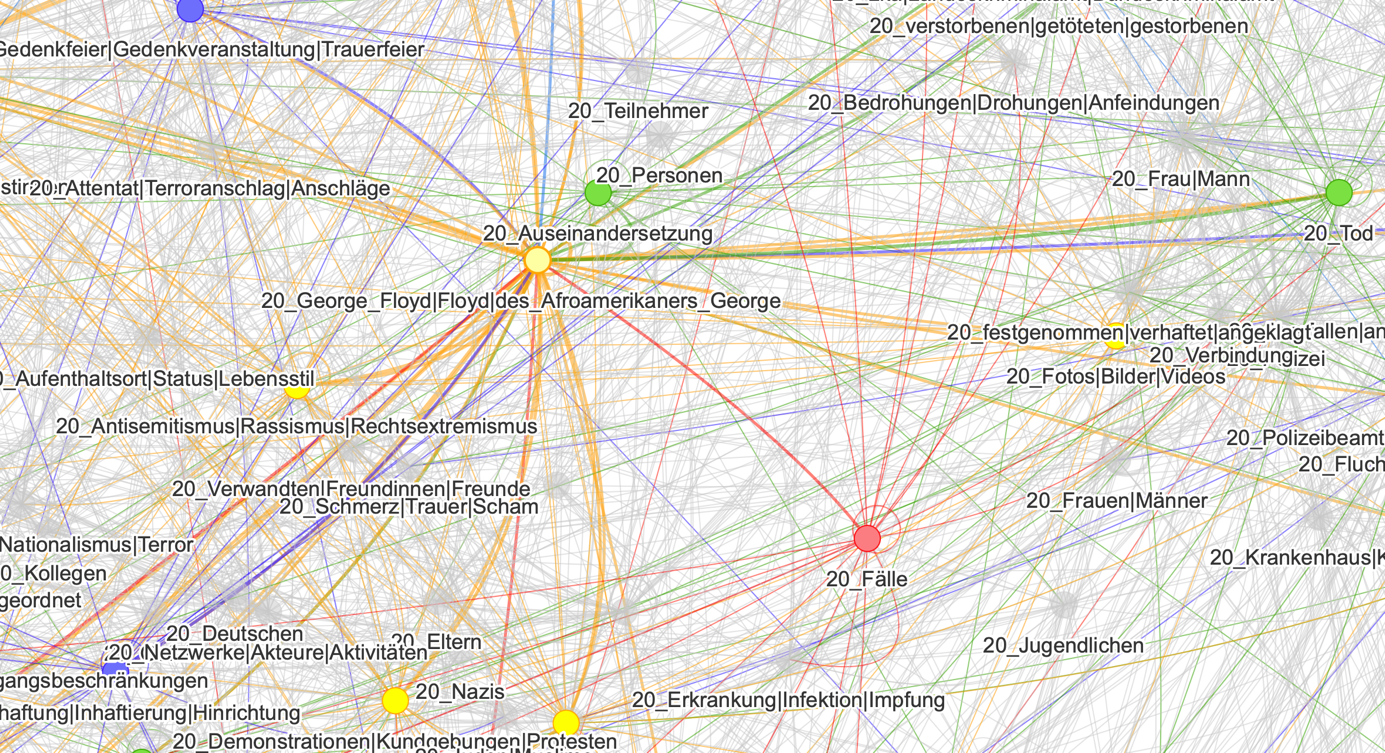
\includegraphics[width=\textwidth]{figures/media/image36.png}
  \caption{\label{fig:george-floyd-frame}Teil des George-Floyd-Frames.}
\end{figure}

Des Weiteren wird mit dem FE \cluster{20\_George\_Floyd{\breakbar}Floyd{\breakbar}des\_Afroamerikaners\_George} erneut ein Fall von in den USA gegen Schwarze ausgeübter Polizeigewalt emergent (siehe \figref{fig:george-floyd-frame}). Auch die sich anschließenden \emph{Black-Lives-Matter}-Proteste finden sich wieder. Zum einen im unten noch näher analysierten FE \cluster{20\_Extinction\_Rebellion{\breakbar}Fridays\_for\_Future{\breakbar}aktivistInnen}, zum anderen im Cluster \cluster{20\_Portland{\breakbar}Minneapolis{\breakbar}Nationalgarde}, das einzelne Orte der Proteste sowie die \emph{Nationalgarde} enthält, die in Teilen des Landes eingesetzt wurde, um gegen die Proteste vorzugehen.

Einzelne Akteure des Rechtsextremismus finden sich zudem im FE \cluster{20\_Rechtsextremen{\breakbar}Rechtsextremisten{\breakbar}Neonazis}, wobei auch eine linke Organisation (\emph{Antifa}) sowie die im Rahmen der Corona-Pandemie neu entstehende Querdenken-Bewegung (\emph{Querdenker}) hier enthalten sind. Über die Vernetzung mit anderen FE wird Rechtsextremismus als (zum Teil politisch) organisiertes Phänomen (\cluster{20\_AfD{\breakbar}Partei}, \cluster{20\_Höcke{\breakbar}Kalbitz{\breakbar}Andreas\_Kalbitz}, \cluster{20\_Gruppen, 20\_Mitglieder}) konstruiert, dessen Handlungsspektrum auf Demonstrationen (u.\,a. \cluster{20\_Demonstrationen{\breakbar}Kundgebung{\breakbar}Demo}, \cluster{20\_protestieren{\breakbar}protestierten{\breakbar}demonstrieren}) fokussiert ist, jedoch auch schwere Gewalttaten (\cluster{20\_Attentat{\breakbar}Terroranschlag{\breakbar}Anschläge}, \cluster{20\_Bedrohungen{\breakbar}Drohungen{\breakbar}Anfeindungen {[}hier auch u.\,a. enthalten: \emph{Attacken}, \emph{Übergriffe}, \emph{Gewalttaten}{]})} umfasst.

Am FE \cluster{20\_Antisemitismus{\breakbar}Rassismus{\breakbar}Rechtsextremismus (Kennzeichen des Rechtsextremismus{\slash}Rechtsextremismus)} zeigt sich erneut der Stigmacharakter des Extremismuskonzeptes (\cluster{20\_Vorwurf}, \cluster{20\_vorgeworfen}). Auch Sicherheitsbehörden wie die \cluster{20\_Polizei} werden wieder als Träger rechtsextremistischer Merkmale diskutiert (siehe Belege K41--K43 in \tabref{tab:K41-K43}).

\begin{table}[t]
  \caption{Konkordanzen zur Kollokation der Cluster \cluster{20\_Antisemitismus{\breakbar}Rassismus{\breakbar}Rechtsextremismus} und \cluster{20\_Polizei}.}
  \label{tab:K41-K43}
K41 taz\_4934582
\begin{tabularx}{\textwidth}{QQQ}
\toprule
Debatte über & {[}\cluster{20\_Antisemitismus{\breakbar}Rassismus{\breakbar}Rechtsextremismus}: \textbf{Rassismus}{]}\newline
\textbf{in}\newline
{[}\cluster{20\_Polizei}: \textbf{Polizei}{]} & wissen wir seit den NSU-Morden Spd-chefin\_Saskia\_Esken wird für ihren Satz unter Polizistinnen in Deutschland gebe \\
\bottomrule
\end{tabularx}
\bigskip \newline
K42 taz\_4952496
\begin{tabularx}{\textwidth}{QQQ}
\toprule
Polizeisprecher über Rassimus wir nehmen keine Hautfarbe fest Thilo\_Cablitz weiß dass es auch bei der & {[}\cluster{20\_Polizei}: \textbf{Polizei}{]}\newline
\newline
{[}\cluster{20\_Antisemitismus{\breakbar}Rassismus{\breakbar}Rechtsextremismus}: \textbf{Rassismus}{]} & gibt aber das sei keinesfalls die Regel sagt der Chef der Pressestelle der Polizei Berlin \\
\bottomrule
\end{tabularx}
\bigskip \newline
K43 taz\_5230564
\begin{tabularx}{\textwidth}{QQQ}
\toprule
die Rede von der kritischen Unabhängigkeit immer mehr zur Farce wird ausgerechnet ein Buch das & {[}\cluster{20\_Antisemitismus{\breakbar}Rassismus{\breakbar}Rechtsextremismus}: \textbf{Rechtsextremismus}{]}\newline
\textbf{in} \textbf{der}\newline
{[}\cluster{20\_Polizei}: \textbf{Polizei}{]} & adressiert denn nachdem das BMI der bpb letzthin eine Links­extremismusdefinition des Verfassungsschutzes diktiert hat hat \\
\bottomrule
\end{tabularx}
\end{table}

Auch warum eher unerwartet das FE \cluster{20\_Meghan{\breakbar}Prinz\_Harry{\breakbar}Harry} hier als Teil des Extremismusdiskurses aufscheint, wird durch die Anbindung an Charakteristika des Rechtsextremismus deutlich. So warfen Prinz Harry und seine Frau Meghan Markle der britischen Königsfamilie Rassismus vor (siehe Belege K44--K46 in \tabref{tab:K44-K46}).

\begin{table}
  \caption{Konkordanzen zur Kollokation der Cluster \cluster{20\_Meghan{\breakbar}Prinz\_Harry{\breakbar}Harry} und \cluster{20\_Antisemitismus{\breakbar}Rassismus{\breakbar}Rechtsextremismus}.}
  \label{tab:K44-K46}
K44 spiegel\_5184036
\begin{tabularx}{\textwidth}{QQQ}
\toprule
erhoben sie im März schwere\_Vorwürfe\_gegen das Königshaus von dem sie sich nicht ausreichend unterstützt fühlten & {[}\cluster{20\_Meghan{\breakbar}Prinz\_Harry{\breakbar}Harry}: \textbf{Meghan}{]}\newline
\textbf{beklagte zudem}\newline
{[}\cluster{20\_Antisemitismus{\breakbar}Rassismus{\breakbar}Rechtsextremismus}: \textbf{Rassismus}{]} & im britischen\_Königshaus seitdem gilt das Verhältnis\_zwischen den beiden und dem Rest der Royals als noch \\
\bottomrule
\end{tabularx}
\bigskip \newline
K45 spiegel\_5130368
\begin{tabularx}{\textwidth}{QQQ}
\toprule
Harry wir sind keine rassistische Familie Prinz\_William verteidigt den britischen Palast gegen den Vorwurf des & {[}\cluster{20\_Antisemitismus{\breakbar}Rassismus{\breakbar}Rechtsextremismus}: \textbf{Rassismus}{]}\newline
\textbf{den}\newline
{[}\cluster{20\_Meghan{\breakbar}Prinz\_Harry{\breakbar}Harry}: \textbf{Meghan}{]} & und Harry erhoben hatten ein Gespräch der Brüder über das Thema steht aber offenbar noch \\
\bottomrule
\end{tabularx}
\bigskip \newline
K46 welt\_5208098
\begin{tabularx}{\textwidth}{QQQ}
\toprule
Kinder in einem Aufsehen\_erregenden Interview mit US-Talkshowlegende Oprah\_Winfrey warfen sie dem Königshaus mangelnde\_Rücksichtnahme und sogar & {[}\cluster{20\_Antisemitismus{\breakbar}Rassismus{\breakbar}Rechtsextremismus}: \textbf{Rassismus}{]}\newline
\textbf{vor}\newline
{[}\cluster{20\_Meghan{\breakbar}Prinz\_Harry{\breakbar}Harry}: \textbf{Meghan}{]} & lt100 hat teilweise afroamerikanische\_Wurzeln der Sunken Garden soll eine besondere\_Anziehungskraft auf die Prinzessin ausgeübt haben \\
\bottomrule
\end{tabularx}
\end{table}

Als letztes FE soll mit \cluster{20\_Extinction\_Rebellion{\breakbar}Fridays\_for\_Future{\breakbar}aktivistInnen} ein Cluster in den Blick genommen werden, das unterschiedliche demonstrierende Gruppen umfasst (u.\,a. \emph{Fridays\_for\_Future}, \emph{Extinction\_Rebellion}, \emph{Black\_Lives\_Matter}, \emph{Querdenken}, \emph{Greenpeace}, \emph{Klimabewegung}), die nicht als extremistisch gelten und sich auch nicht ohne Weiteres in die Extremismus-Trias aus Links- und Rechtsextremismus sowie Islamismus einordnen lassen. Die paradigmatische Ähnlichkeit, die das Zu-Tage-Treten im Frame bedingt, liegt in der Organisiertheit (\cluster{20\_Gruppen}, \cluster{20\_Netzwerke, 20\_Organisationen{\breakbar}Initiativen{\breakbar}Stiftungen}, \cluster{20\_Netzwerke{\breakbar}Akteure{\breakbar}Aktivitäten}) und dem außerparlamentarischen Agieren in Form von Protesten und Demonstrationen (u.\,a. \cluster{20\_Widerstand{\breakbar}Protest}, \cluster{20\_Straßen{\breakbar}Straße}, \cluster{20\_Demonstranten}). Es zeigt sich auch eine Anbindung an (insbesondere rechts\mbox{-}) extremistische Akteure (\cluster{20\_Rechtsextremen{\breakbar}Rechtsextremisten{\breakbar}Neonazis}), was einerseits damit zusammenhängt, dass in diesem Cluster auch unspezifischere Ausdrücke wie \emph{Gruppe} oder \emph{Gruppierung} enthalten sind (K47), andererseits auf Interaktionen der unterschiedlichen Akteure miteinander (K48) oder auch die Zuschreibung, rechtsextrem zu sein (K49), zurückgeht (siehe \tabref{tab:K47-K49}).

\begin{table}
  \caption{Konkordanzen zur Kollokation der Cluster \cluster{20\_Extinction\_Rebellion{\breakbar}Fridays\_for\_Future{\breakbar}aktivistInnen} und \cluster{20\_Rechtsextremen{\breakbar}Rechtsextremisten{\breakbar}Neonazis}.}
  \label{tab:K47-K49}
K47 welt\_4825726
\begin{tabularx}{\textwidth}{QQQ}
\toprule
Klimaschutz verhinderten hieß es in Berlin hatten sich Anfang Oktober mehrere\_tausend\_Menschen an einer Aktionswoche von & {[}20\_Extinction\_Rebellion{\breakbar}Fridays\_for\_Future{\breakbar}aktivistInnen: \textbf{Extinction\_Rebellion}{]}\newline
\textbf{beteiligt zu den Strategien der}\newline
{[}20\_Rechtsextremen{\breakbar}Rechtsextremisten{\breakbar}Neonazis: \textbf{Gruppe}{]} & gehören Aktionen\_zivilen\_Ungehorsams wie Flashmobs Fahrraddemos sowie Brücken- und Straßenblockaden zuletzt war die Bewegung auch wegen \\
\bottomrule
\end{tabularx}
\bigskip \newline
K48 spiegel\_4937908
\begin{tabularx}{\textwidth}{QQQ}
\toprule
an diesem Samstag auf dem Trafalgar\_Square musste sich die Polizei einmischen um Zusammenstöße\_zwischen kleineren\_Gruppen von & {[}20\_Rechtsextremen{\breakbar}Rechtsextremisten{\breakbar}Neonazis: \textbf{Rechtsextremen}{]}\newline
\textbf{und Aktivisten von}\newline
{[}20\_Extinction\_Rebellion{\breakbar}Fridays\_for\_Future{\breakbar}aktivistInnen: \textbf{Black\_Lives\_Matter}{]} & zu verhindern die große Anti-rassismus-demonstration war auf Freitag vorverlegt\_worden um sich vor rechten Denkmalschützern zu \\
\bottomrule
\end{tabularx}
\bigskip \newline
K49 taz\_5051588
\begin{tabularx}{\textwidth}{QQQ}
\toprule
mal mit Inhalten beschäftigt man sollte sich lieber mal anhören welche Sprüche und Transparente bei & {[}20\_Extinction\_Rebellion{\breakbar}Fridays\_for\_Future{\breakbar}aktivistInnen: \textbf{Querdenken}{]}\newline
\textbf{dabei sind als zu sagen}\newline
{[}20\_Rechtsextremen{\breakbar}Rechtsextremisten{\breakbar}Neonazis: \textbf{Rechtsextremisten}{]} & würden das unterwandern ich sehe dort eine Menge rechtsextremes\_Gedankengut bei Leuten die als solche nicht \\
\bottomrule
\end{tabularx}
\end{table}

\subsubsection{Islamismus}\label{islamismus-7}

Der Bereich des Islamismus erscheint in diesem Zeitraum eher wenig ausdifferenziert. Insgesamt ist sogar zu beobachten, dass auch ein FE wie \cluster{20\_Attentat{\breakbar}Terroranschlag{\breakbar}Anschläge}, das (bzw. dessen äquivalente Cluster) in den anderen Zeiträumen eng mit dem Bereich ‚Krieg \& Islamismus` assoziiert war, nun mehr Verbindungen in andere Teile des Gesamt-Frames und mithin zu rechtsextremen Anschlägen aufweist. Ähnlich, wenn auch insgesamt noch stärker an den Bereich des Islamismus gebunden, verhält es sich mit dem FE \cluster{20\_Anschlag{\breakbar}Angriff}. Stark vernetzt im Bereich ‚Krieg \& Islamismus` ist hingegen die \cluster{20\_Taliban}, die nach dem durch die USA initiierten (\cluster{20\_Us-regierung}, \cluster{20\_Usa{\breakbar}Vereinigten\_Staaten}) Rückzug der NATO aus Afghanistan (\cluster{20\_Rückzug{\breakbar}Austritt{\breakbar}Ausstieg}) wieder die Macht (\cluster{20\_Macht}, \cluster{20\_Kontrolle}) im Land übernahm, woraufhin es am Kabuler \cluster{20\_Flughafen} zu chaotischen Zuständen kam.

\subsubsection{Fazit}\label{fazit-7}

Insgesamt zeigt der Extremismus-Frames des Zeitraums 2020--2021 ein Framing, das insbesondere Rechtsextremismus ausdifferenziert und in Hinblick auf unterschiedliche thematische Dimensionen konturiert. Dabei werden einerseits politische Zusammenhänge um den ausgewiesen rechtsextremistischen Flügel in der AfD sowie die Thüringer Ministerpräsidentenwahl 2020 Teil des Frames, zum anderen auch mehrere rechtsextremistisch motivierte Anschläge und ihre juristische, aber auch gesellschaftliche Aufarbeitung in Form von Gedenkveranstaltungen und Anteilnahme. Es fällt außerdem auf, dass terroristische Anschläge nun ein wesentlicher Teil des rechtsextremistischen Handlungsspektrums geworden und nicht mehr in erster Linie mit dem Islamismus assoziiert sind. Mit der Querdenken-Bewegung findet sich darüber hinaus eine neu entstandene Gruppierung in den FE wieder, die teils eher mit anderen Gruppen des außerparlamentarischen Protests (\emph{Querdenken} in \cluster{20\_Extinction\_Rebellion{\breakbar}Fridays\_for\_Future{\breakbar}aktivistInnen}), teils eher mit klar extremistischen Gruppierungen (\emph{Querdenker} in \cluster{20\_Rechtsextremen{\breakbar}Rechtsextremisten{\breakbar}Neonazis}) paradigmatisch assoziiert ist. Während im Fall von Querdenken bereits im Untersuchungszeitraum eine Beobachtung durch den Verfassungsschutz erfolgt und Überlappungen mit rechtsextremistischen Gruppen bzw. rechtsextremistischem Gedankengut thematisiert werden (Konkordanz K49), sind etwa \emph{Extinction Rebellion} und \emph{Fridays for Future} nicht gleichermaßen unter Extremismusverdacht, aber dennoch Teil des Frames. Der Grund hierfür liegt wohl darin, dass sie mit Demonstrationen eine Aktionsform nutzen, die -- das ist in jedem der betrachteten Zeiträume deutlich geworden -- auch für politisch-extremistische Gruppierungen typisch ist. Diese bereits vorhandene paradigmatische Ähnlichkeit der Gruppen im Diskurs könnte gewissermaßen den Boden für ein Framing als extremistische Akteure ebnen, das sich etwa in Bezug auf die Letzte Generation nach dem Untersuchungszeitraum noch deutlicher zeigen wird und in dem durch namhafte Politiker Vergleiche mit der RAF oder Taliban gezogen werden.\footnote{So sagte der CSU-Landesgruppenchef Alexander Dobrindt der \textsc{Bild am Sonntag} in Bezug auf die Letzte Generation, es müsse die „Entstehung einer Klima-RAF`` verhindert werden (\url{https://www.bild.de/politik/inland/politik-inland/knallhart-kurs-gegen-klima-chaoten-union-will-knast-statt-geldstrafen-81844836.bild.html} {[}18.12.2025{]}), und der SPD-Politiker Michael Roth kommentierte in einem (mittlerweile gelöschten) Tweet „Was für eine billige, würdelose Aktion. Ihr scheißt auf Grundrechte, zerstört Kunst ähnlich wie die Taliban und fühlt Euch noch als Heldinnen und Helden!{}``.}

Im Bereich des Islamismus lassen sich keine größeren Brüche im Framing konstatieren. Inhaltlich zeichnet sich insbesondere der Rückzug des Westens aus Afghanistan und die daraufhin erfolgende Machtergreifung durch die Taliban ab.

\subsection{\texorpdfstring{\textsc{Taz}}{Taz}}\label{taz}


\subsubsection{\texorpdfstring{\emph{Corpus-driven} Voranalyse: Thematisch gruppierte Auswahl semantisch äquivalenter Cluster im Vergleich zu den Kern-FE der diachronen Analyse}{Corpus-driven Voranalyse: Thematisch gruppierte Auswahl semantisch äquivalenter Cluster im Vergleich zu den Kern-FE der diachronen Analyse}}\label{corpus-driven-voranalyse-thematisch-gruppierte-auswahl-semantisch-aequivalenter-cluster-im-vergleich-zu-den-kern-fe-der-diachronen-analyse}
Nachdem die vorigen Kapitel das Framing einzelner Extremismusvarianten auf der diachronen Achse kontrastiert haben und die einzelnen Zeitungen dabei aggregiert waren, wird das Korpus im Folgenden entlang der medial-kontrastiven Achse geteilt und untersucht. Wie in \chapref{vorgehen-und-zielsetzung} beschrieben, erfolgen dabei ebenfalls quantitative Voranalysen. Die Analyse äquivalenter Cluster (siehe Tabelle 10 im Anhang) baut auf den Ergebnissen aus der diachronen Analyse auf und ermittelt äquivalente Cluster zu allen Kern-FE der untersuchten Zeiträume und fasst diese -- wie zuvor -- thematisch gruppiert in je einer Tabelle zusammen (siehe Tabellen \ref{tab:taz_1}--\ref{tab:taz_3}).

\begin{table}\small
\caption{Thematisch gruppierte Auswahl semantisch äquivalenter Cluster der \textsc{TAZ}.}
\label{tab:taz_1}
 \begin{tabularx}{\textwidth}{>{\hsize=0.5\hsize}X >{\hsize=0.5\hsize}X >{\hsize=2.0\hsize}X}
  \lsptoprule
  Extremismus-Variante & Bezug & Frame-Elemente \\
  \midrule
  \multirow{2}{=}{Rechts\-ex\-tre\-mis\-mus} 
  & historisch & \cluster{1945{\breakbar}Kriegsende, Nationalsozialismus, Vernichtungslager{\breakbar}Konzentrationslager{\breakbar}Kz, Deportationen{\breakbar}Konzentrationslagern{\breakbar}Deportation, Wehrmacht{\breakbar}Roten\_Armee{\breakbar}Sowjets, Nazis, Holocaust, Nazideutschland{\breakbar}Nazi-deutschland{\breakbar}nationalsozialistischen, Wehrmachtssoldaten{\breakbar}Kz-häftlinge{\breakbar}Deserteure, Nazizeit{\breakbar}Ns-zeit{\breakbar}Weimarer\_Republik} \\
  & zeit\-ge\-nössisch & \cluster{Rassisten{\breakbar}Antisemiten{\breakbar}Faschisten, Afd{\breakbar}Npd, Dvu, Alexander\_Gauland{\breakbar}Jörg\_Meuthen{\breakbar}Poggenburg, Schill{\breakbar}Schill-Partei, Nsu, Hooligans{\breakbar}Fußballfans{\breakbar}Ultras, Gauland{\breakbar}Höcke{\breakbar}Meuthen, Zschäpe{\breakbar}Beate\_Zschäpe, rechtsradikale{\breakbar}rechtsextreme{\breakbar}antisemitische, Diskriminierung, Islamophobie{\breakbar}Xenophobie{\breakbar}Islamfeindlichkeit, Antisemitismus{\breakbar}Rassismus, Rechtsextremisten{\breakbar}Neonazis{\breakbar}Rechtsextremen, ausländerfeindliche{\breakbar}fremdenfeindliche{\breakbar}fremdenfeindlichen} \\
  \lspbottomrule
 \end{tabularx}
\end{table}

 \begin{table}[b]\small
\caption{Thematisch gruppierte Auswahl semantisch äquivalenter Cluster der \textsc{TAZ}.}
\label{tab:taz_2}
 \begin{tabularx}{\textwidth}{>{\hsize=0.5\hsize}X >{\hsize=0.5\hsize}X >{\hsize=2.0\hsize}X}
  \lsptoprule
  Extremismus-Variante & Bezug & Frame-Elemente \\
  \midrule
  \multirow{2}{=}{Links\-ex\-tre\-mis\-mus} 
  & historisch & \cluster{Milošević, Stasi{\breakbar}Staatssicherheit} \\
  & zeit\-ge\-nössisch & \cluster{linksradikalen{\breakbar}marxistischen{\breakbar}anarchistischen, Pds{\breakbar}Linkspartei, Antifa-gruppen{\breakbar}Aktivistinnen{\breakbar}linke\_Gruppen, Linke, Gegendemonstranten{\breakbar}Randalierer{\breakbar}Einsatzkräfte, Oskar\_Lafontaine{\breakbar}Gregor\_Gysi, Heiligendamm{\breakbar}Genua{\breakbar}G-8-Gipfel, gegen\_Rechts{\breakbar}antifaschistische{\breakbar}Antifa} \\
  \midrule
  \multirow{2}{=}{Politischer Extremismus} 
  & historisch & \cluster{Kpd{\breakbar}Nsdap{\breakbar}Sed, Kommunismus{\breakbar}Sozialismus{\breakbar}Faschismus, Hitler{\breakbar}Adolf\_Hitler{\breakbar}Stalin, ermordeten\_Juden{\breakbar}Reichspogromnacht{\breakbar}Ns-opfer} \\
  & zeit\-ge\-nössisch & \cluster{Rechtspopulismus{\breakbar}Populisten{\breakbar}Populismus, rechten\_Szene{\breakbar}rechtsextremen\_Szene{\breakbar}linken\_Szene, Antifas{\breakbar}Skins{\breakbar}Antifaschisten, Npd-kundgebung{\breakbar}Neonazi-Demo{\breakbar}NPD-Demo} \\
  \lspbottomrule
 \end{tabularx}
\end{table}

 \begin{table}[b]\small
\caption{Thematisch gruppierte Auswahl semantisch äquivalenter Cluster der \textsc{TAZ}.}
\label{tab:taz_3}
 \begin{tabularx}{\textwidth}{>{\hsize=0.5\hsize}X >{\hsize=0.5\hsize}X >{\hsize=2.0\hsize}X}
  \lsptoprule
  Extremismus-Variante & Bezug & Frame-Elemente \\
  \midrule
  {Islamismus} & Nahost\-konflikt & \cluster{jüdischen\_Siedlungen{\breakbar}Palästinensergebiete{\breakbar}Golanhöhen, Arbeitspartei{\breakbar}Ehud\_Barak{\breakbar}Benjamin\_Netanjahu, Palästinenserpräsident\_Mahmud\_Abbas{\breakbar}Palästinenserpräsident\_Jassir\_Arafat{\breakbar}Jassir\_Arafat, iS, Israel{\breakbar}Palästina, israelische{\breakbar}palästinensische, israelischen{\breakbar}palästinensischen, Palästinenser{\breakbar}Israelis, Ramallah{\breakbar}Jerusalem{\breakbar}Gaza, Scharon{\breakbar}Arafat{\breakbar}Barak, Gaza-streifen{\breakbar}Gazastreifen{\breakbar}Westjordanland, Hebron{\breakbar}Nablus{\breakbar}Dschenin, Palästinenserpräsident\_Arafat{\breakbar}Präsident\_Mahmud\_Abbas{\breakbar}Abu\_Masen} \\
  & Kriege Naher{\slash}Mittlerer Osten & \cluster{Mossul{\breakbar}Falludscha{\breakbar}Homs, Syrien{\breakbar}Libyen{\breakbar}Afghanistan, Huthis{\breakbar}Baschar\_al-Assad{\breakbar}Sadr, Iraks{\breakbar}Libyens{\breakbar}Syriens, syrischen{\breakbar}libanesischen{\breakbar}irakischen, syrische{\breakbar}irakische{\breakbar}iranische} \\
  & Terrorismus & \cluster{Bin\_Laden{\breakbar}Ussama\_Bin\_Laden{\breakbar}al-Qaida, Hisbollah{\breakbar}Hamas{\breakbar}Pkk, Al-kaida{\breakbar}Al-Qaida{\breakbar}Isis, mutmaßlichen\_Terroristen{\breakbar}Al-Qaida-Mitglieder{\breakbar}Bombenleger} \\
  & Weiteres & \cluster{Mursi{\breakbar}Chatami{\breakbar}Mubarak, Saddam\_Hussein{\breakbar}Gaddafi{\breakbar}Saddam, Extremisten{\breakbar}Islamisten{\breakbar}Dschihadisten, schiitischen{\breakbar}sunnitischen{\breakbar}sunnitische, Muslimbrüder{\breakbar}Radikalen{\breakbar}Muslimbruderschaft} \\
  \midrule
  varianten\-über\-greifend & & \cluster{Gorleben, Rechtsradikalismus{\breakbar}Fremdenfeindlichkeit{\breakbar}Extremismus} \\
  \lspbottomrule
 \end{tabularx}
\end{table}

\subsubsection{\texorpdfstring{\emph{Corpus-driven} Voranalyse: Cluster mit hoher Cosinus-Distanz im Vergleich zum Gesamtkorpus}{Corpus-driven Voranalyse: Cluster mit hoher Cosinus-Distanz im Vergleich zum Gesamtkorpus}}\label{corpus-driven-voranalyse-cluster-mit-hoher-cosinus-distanz-im-vergleich-zum-gesamtkorpus-1}


Es wurde auch im Rahmen der medienkontrastiven Analyse ermittelt, welche Cluster die höchsten Cosinus-Distanzen im Vergleich zum Gesamtmodell aufweisen. Die Ergebnisse sind jedoch kaum fruchtbar zu interpretieren (siehe \tabref{tab:cluster-high-cosine-distance-taz}). So zeigt sich, dass die Cosinus-Distanzen in der \textsc{Taz} wesentlich geringer ausfallen als bei den zu den Vorjahreszeiträumen vorgenommenen Vergleichen, die regelmäßig Distanzen von über 0,4 aufwiesen. Weniger groß fällt die Diskrepanz zu den ebenfalls zum Gesamtmodell berechneten Distanzen im Zeitraum 1999--2001 aus (max. 0,28). Insgesamt scheinen also sowohl aufgrund des sehr großen Vergleichskorpus als auch im medialen Vergleich geringere Unterschiede im Framing der Zeitungen aufzutreten. Ein weiteres Problem besteht darin, dass die Cluster aufgrund der Größe der einzelnen Zeitungskorpora deutlich mehr Ausdrücke umfassen und mithin schwieriger zu interpretieren sind. Außerdem bestehen Cluster der einen Zeitung oft nicht in den anderen Zeitungen, was einen Vergleich erschwert. Im Folgenden werden daher nur die in \chapref{vorgehen-und-zielsetzung} festgelegten FE einer kontrastiven Analyse unterzogen.

\begin{table}[t]\small
\caption{Cluster mit hoher Cosinus-Distanz im Vergleich zum vorigen Zeitraum.}
\label{tab:cluster-high-cosine-distance-taz}
\begin{tabularx}{\textwidth}{X r}
\lsptoprule
Cluster & Cos.-Dist. \\
\midrule
\cluster{Schiedsverfahren{\breakbar}Klageverfahren{\breakbar}Musterverfahren} & 0.22 \\
\cluster{Raubüberfall{\breakbar}schweren\_Unfall{\breakbar}Messerangriff} & 0.22 \\
\cluster{Afghanistankrieg{\breakbar}Kosovokrieg{\breakbar}Kosovo-Krieg} & 0.21 \\
\cluster{Kauder{\breakbar}Glos{\breakbar}Csu-chef\_Horst\_Seehofer} & 0.21 \\
\cluster{20-Jährigen{\breakbar}18-Jährigen{\breakbar}19-Jährigen} & 0.21 \\
\cluster{Us-außenminister\_Colin\_Powell{\breakbar}US-Außenministerin\_Condoleezza\_Rice{\breakbar}US-Außenministerin\_Hillary\_Clinton} & 0.21 \\
\cluster{Neuerkrankungen{\breakbar}Sterbefälle{\breakbar}Hiv-infektionen} & 0.21 \\
\cluster{Militäreinsatz{\breakbar}Militärschlag{\breakbar}Angriffskrieg} & 0.21 \\
\cluster{Beckstein{\breakbar}Söder{\breakbar}Schily} & 0.21 \\
\cluster{Barroso{\breakbar}Eu-kommissionspräsident\_Jean-claude\_Juncker{\breakbar}Tusk} & 0.21 \\
\cluster{Passierschein{\breakbar}Aufenthaltstitel{\breakbar}richterlichen\_Beschluss} & 0.2 \\
\cluster{offiziellen\_Stellungnahme{\breakbar}ähnlichen\_Situation{\breakbar}gemeinsamen\_Stellungnahme} & 0.2 \\
\cluster{John\_Edwards{\breakbar}Newt\_Gingrich{\breakbar}Marco\_Rubio} & 0.2 \\
\cluster{Opportunisten{\breakbar}Ideologen{\breakbar}Idealisten} & 0.2 \\
\cluster{Landesinneren{\breakbar}Süden\_Somalias{\breakbar}Südirak} & 0.2 \\
\cluster{Flugabwehrraketen{\breakbar}Luftabwehrraketen{\breakbar}Marschflugkörpern} & 0.2 \\
\cluster{Einzelmaßnahmen{\breakbar}Festlegungen{\breakbar}Zielvorgaben} & 0.2 \\
\cluster{Besatzer{\breakbar}Befreier{\breakbar}Imperialisten} & 0.2 \\
\cluster{Mousli{\breakbar}Motassadeq{\breakbar}Wüppesahl} & 0.19 \\
\cluster{Bouteflika{\breakbar}Tshisekedi{\breakbar}Obasanjo} & 0.19 \\
\lspbottomrule
\end{tabularx}
\end{table}

\subsubsection{Rechts- und Linksextremismus}\label{rechts--und-linksextremismus-8}

Die in den Tabellen \ref{tab:taz_1} und \ref{tab:taz_2} vorgenommene grobe Zuordnung der FE zu einzelnen Extremismusvarianten zeigt, dass für das \textsc{Taz}-Teilkorpus -- anders als in der Mehrzahl der diachronen Subkorpora -- mehrere FE emergieren, die sich einem (zeitgenössischen) Linksextremismus-Frame zuordnen lassen. Es finden sich des Weiteren zwei Cluster, die eher historische Dimensionen des Linksextremismus abbilden sowie eine Vielzahl an Clustern, die einen Rechtsextremismus-Frame sowohl historisch als auch kontemporär konstituieren.

In Parteien organisierte Formen des Rechtsextremismus finden sich in den Clustern \cluster{ta\_Afd{\breakbar}Npd}, \cluster{ta\_Dvu}, \cluster{ta\_Schill{\breakbar}Schill-Partei}, \cluster{ta\_Gauland{\breakbar}Höcke{\breakbar}Meuthen (AfD-Politiker{\slash}Möllemann)} sowie \cluster{ta\_Alexander\_Gauland{\breakbar}Jörg\_Meuthen{\breakbar}Poggenburg (Rechtsaußen-Politiker)}. Diese zeigen insgesamt ein Framing, das einerseits auf den für Parteien üblichen FE im Netzwerk-Cluster ‚Politik` beruht, andererseits jedoch auch stark -- insbesondere durch das FE \cluster{ta\_Afd{\breakbar}Npd} -- an den thematischen Bereich ‚Demonstrationen \& Politischer Extremismus` anknüpft. Hier treten zum einen die deutliche Assoziation mit extremistischen Akteuren und Attributen (\cluster{ta\_Rassisten{\breakbar}Antisemiten{\breakbar}Faschisten}, \cluster{ta\_Rechtsradikalismus{\breakbar}Fremdenfeindlichkeit{\breakbar}Extremismus}, \cluster{ta\_gegen\_Rechts{\breakbar}antifaschistische{\breakbar}Antifa}, \cluster{ta\_Rechten}, \cluster{ta\_ausländerfeindliche{\breakbar}fremdenfeindliche{\breakbar}fremdenfeindlichen}, \cluster{ta\_Rechtsextremisten{\breakbar}Neonazis{\breakbar}Rechtsextremen}, \cluster{ta\_rechten\_Szene{\breakbar}rechtsextremen\_Szene{\breakbar}linken\_Szene}), zum anderen das Agieren im Rahmen von Demonstrationen bzw. Protesten (\cluster{ta\_Marsch}, \cluster{ta\_Parolen{\breakbar}Slogans}, \cluster{ta\_Protest\_gegen}, \cluster{ta\_Demonstration{\breakbar}Demo}, \cluster{ta\_Veranstaltung{\breakbar}Aktion}, \cluster{ta\_Kundgebung}) hervor. Es finden sich des Weiteren mehrere FE im thematischen Teil-Frame ‚Straftaten \& Juristisches`, die etwa einzelne Straftaten (\cluster{ta\_Urkundenfälschung{\breakbar}Freiheitsberaubung{\breakbar}Widerstand\_gegen\_Vollstreckungsbeamte}, \cluster{ta\_wegen\_Urkundenfälschung{\breakbar}schwerer\_Körperverletzung{\breakbar}wegen\_räuberischer\_erpressung}), aber auch den Verfassungsschutz (\cluster{ta\_Verfassungsschutz}) und dessen Ermittlungen (\cluster{ta\_Spitzel{\breakbar}Informanten{\breakbar}V}-mann) sowie das Bundesverfassungsgericht (\cluster{ta\_Bundesverfassungsgericht}) und Fragen der Organisationsmitgliedschaft (\cluster{ta\_Mitgliedschaft}) zum Teil des verstehensrelevanten Wissens machen. Der Hintergrund liegt dabei etwa in den bereits in der diachronen Analyse berichteten Zusammenhängen um das NPD-Verbotsverfahren, der Relevanz der Mitgliedschaft in extremistischen Gruppen oder Parteistrukturen sowie der erfolgenden Beobachtung durch den Verfassungsschutz vor dem Hintergrund einer möglichen institutionellen Einstufung als extremistisch.
\largerpage

Als weiterer zentraler Teil der diachronen Rechtsextremismus-Frames soll der NSU in den Blick genommen werden, der insbesondere durch die FE \cluster{ta\_Nsu} und \cluster{ta\_Zschäpe{\breakbar}Beate\_Zschäpe} repräsentiert ist. Der sich aus diesen FE ergebende Teil-Frame zeigt eine starke Vernetzung im Bereich ‚Straftaten \& Juristisches`, was einerseits auf den sich über viele Jahre erstreckenden NSU-Prozess zurückgeht (u.\,a. \cluster{ta\_angeklagt}, \cluster{ta\_Angeklagten{\breakbar}Angeklagte}, \cluster{ta\_Anwalt}, \cluster{ta\_Gericht}), andererseits auf die verübten Gewalttaten (u.\,a. \cluster{ta\_Morden}, \cluster{ta\_Bluttat{\breakbar}Fahndung{\breakbar}Anschlagsserie}) und die Ermittlungen bzw. die Aufklärung des Ermittlungsversagens (u.\,a. \cluster{ta\_Recherchen}, \cluster{ta\_Akten{\breakbar}Unterlagen}, \cluster{ta\_Spitzel{\breakbar}Informanten{\breakbar}V-mann}, \cluster{ta\_Untersuchungsausschuss}, \cluster{ta\_Versäumnisse{\breakbar}Mängel{\breakbar}Defizite}). Relativ undeutlich ist hingegen das explizite Framing des NSU als rechtsextremistische Gruppierung. So finden sich keine Verbindungen zu den FE, die die zuvor besprochenen rechten Parteien als extremistisch ausweisen.\footnote{Ein möglicher Grund für das Ausbleiben (sehr starker) Kollokationen könnte -- zumindest für die Kollokationsrichtung des Clusters \cluster{ta\_Rechtsextremisten{\breakbar}Neonazis{\breakbar}Rechtsextremen} zum NSU darin liegen, dass ersteres Cluster im gesamten Untersuchungszeitraum auftritt, während die NSU-Cluster erst ab 2011 im Diskurs vorkommen. Ausdrücke, die über den gesamten Zeitraum kookkurrieren haben insofern eine größeres Potenzial, Kollokationen zu bilden.}

Für eine kontrastive Analyse der Zeitungen wurde des Weiteren das FE \cluster{ta\_Rechtsextremisten{\breakbar}Neonazis{\breakbar}Rechtsextremen} ausgewählt, das in der \textsc{Taz} über die im Label enthaltenen Wörter hinaus nur das Wort \emph{Rechtsextreme} enthält und mithin Akteure des Rechtsextremismus auf einer recht allgemeinen, auf das Phänomen ‚Rechtsextremismus` bezogenen Ebene benennt. Das Framing spielt sich insbesondere im thematischen Bereich ‚Demonstrationen \& politischer Extremismus` ab. Hier zeigen angeschlossene FE wie \cluster{ta\_Hooligans{\breakbar}Fußballfans{\breakbar}Ultras} und \cluster{ta\_Rassisten{\breakbar}Antisemiten{\breakbar}Faschisten} Möglichkeiten der Perspektivierung bzw. epistemischen Spezifizierung auf; beim Erstgenannten in Hinblick auf eine im Fußballkontext aktive Teilgruppe, bei Zweiterem in Hinblick auf ideologische Aspekte. Wie bereits in der diachronen Analyse gezeigt, ist ein weiteres wesentliches Merkmal des Framings von Extremismusvarianten die Organisationsform, die hier in FE wie \cluster{ta\_rechten\_Szene{\breakbar}rechtsextremen\_Szene{\breakbar}linken\_Szene}, \cluster{ta\_Kontakte{\breakbar}Verbindungen} und \cluster{ta\_Gruppe} emergiert. Ein weiterer wesentlicher Anteil entfällt auf das Demonstrieren als typische Handlungsform des politischen Extremismus, u.\,a. in den FE \cluster{ta\_Protest\_gegen}, \cluster{ta\_Parolen{\breakbar}Slogans}, \cluster{ta\_Kundgebung}, \cluster{ta\_Mahnwache}. Dem Handeln der rechtsextremistischen Akteure wird dabei eine strategische Ausrichtung zugesprochen (\cluster{ta\_Strategie{\breakbar}Taktik}, \cluster{ta\_Aktivitäten{\breakbar}Bestrebungen}, \cluster{ta\_gezielt{\breakbar}systematisch}). In den Themenfeldern ‚Krieg \& Islamismus` sowie ‚Straftaten \& Juristisches` zeigen sich darüber hinaus FE, die das Verüben physischer Gewalt (\cluster{ta\_Schießerei{\breakbar}Schlägerei}, \cluster{ta\_verprügelt{\breakbar}zusammengeschlagen{\breakbar}attackiert}, \cluster{ta\_Gewalttaten{\breakbar}Übergriffe{\breakbar}Straftaten}, \cluster{ta\_verübten{\breakbar}verübte{\breakbar}verübten}) und institutionelles Vorgehen (\cluster{ta\_Razzia}, \cluster{ta\_Polizei}) anzeigen. Eine räumliche Verortung des Rechtsextremismus leisten die FE \cluster{ta\_mehreren\_Bundesländern{\breakbar}mehreren\_Städten{\breakbar}allen\_Bundesländern} und \cluster{ta\_Hochburg}. Letzteres FE ist dabei im Bereich ‚Krieg \& Islamismus` angesiedelt und wird auch in Bezug auf terroristische Organisationen verwendet (u.\,a. \cluster{ta\_iS}, \cluster{ta\_Al-kaida{\breakbar}Al-Qaida{\breakbar}Isis}), was eine paradigmatische Ähnlichkeit zwischen den beiden Extremismusformen konstituiert. Es finden sich des Weiteren Bezüge zum Bereich des Linksextremismus. So zeigen die Kookkurrenzen mit den linken Akteuren des FE \cluster{ta\_Antifas{\breakbar}Skins{\breakbar}Antifaschisten}, das Akteure des Links- und Rechtsextremismus vereint, insbesondere ein durch Konfrontation und Gewalt geprägtes Bild (siehe Belege K50--K52 in \tabref{tab:K50-K52}).

\begin{table}
\caption{Konkordanzen zur Kollokation der Cluster \cluster{ta\_Rechtsextremisten{\breakbar}Neonazis{\breakbar}Rechtsextremen} und \cluster{ta\_Antifas{\breakbar}Skins{\breakbar}Antifaschisten} in der \textsc{Taz}.}
\label{tab:K50-K52}
K50 taz\_202385
\begin{tabularx}{\textwidth}{QQQ}
\toprule
sie gekommen waren per S-bahn am Abend kam es am Hauptbahnhof zu einer Schlägerei zwischen & {[}\cluster{ta\_Rechtsextremisten{\breakbar}Neonazis{\breakbar}Rechtsextremen}: \textbf{Neonazis}{]}\newline
\textbf{und etwa lt1000}\newline
{[}\cluster{ta\_Antifas{\breakbar}Skins{\breakbar}Antifaschisten} :\textbf{Autonomen}{]} & die Polizei schloss die Linken ein und nahm zwei von ihnen fest ein Polizist und \\
\bottomrule
\end{tabularx}
\bigskip \newline
K51 taz\_3426012
\begin{tabularx}{\textwidth}{QQQ}
\toprule
Opfern\_rechter\_Gewalt gewidmet ist bisher fand die Demo stets in Friedrichshain statt dort wo der linke & {[}\cluster{ta\_Antifas{\breakbar}Skins{\breakbar}Antifaschisten}: \textbf{Hausbesetzer}{]}\newline
\textbf{Meier 1992 von}\newline
{[}\cluster{ta\_Rechtsextremisten{\breakbar}Neonazis{\breakbar}Rechtsextremen}: \textbf{Neonazis}{]} & ermordet wurde über die Jahre ist der jährliche\_Gedenkmarsch zu einer Art Familientreff der linken\_Szene im \\
\bottomrule
\end{tabularx}
\bigskip \newline
K52 taz\_5040538
\begin{tabularx}{\textwidth}{QQQ}
\toprule
nach Angriff auf & {[}\cluster{ta\_Rechtsextremisten{\breakbar}Neonazis{\breakbar}Rechtsextremen}: \textbf{Rechtsextreme}{]}\newline
\newline
{[}\cluster{ta\_Antifas{\breakbar}Skins{\breakbar}Antifaschisten} : \textbf{Autonomen}{]} & in Leipzig festgenommen die Bundesanwaltschaft durchsucht drei Leipziger Linksradikale und nimmt eine Frau fest Sie \\
\bottomrule
\end{tabularx}
\end{table}

In der \textsc{Taz} bilden sich außerdem-- im Gegensatz zu den anderen Zeitungen -- gleich mehrere für den Linksextremismus einschlägige FE, die näher besprochen werden sollen. Darunter markieren \cluster{ta\_Linke}, \cluster{ta\_Pds{\breakbar}Linkspartei} und \cluster{ta\_Oskar\_Lafontaine{\breakbar}Lafontaine{\breakbar}Gregor\_Gysi} politische Akteure im Netzwerk-Cluster ‚Politik`, in dem die Linke ohne größere Auffälligkeiten als politische Partei semantisiert wird. In den anderen thematischen Frame-Anteilen finden sich hingegen FE, die einen besonderen Status der Partei andeuten: So weist sie eine Relation zum FE \cluster{ta\_Afd{\breakbar}Npd} aus dem Bereich ‚Demonstrationen \& politischer Extremismus` auf sowie zum FE \cluster{ta\_Kpd{\breakbar}Nsdap{\breakbar}Sed} aus einem thematischen Teil-Frame, in dem es um die NS-Zeit und schwere historische Verbrechen geht. Dem gemeinsamen Auftreten mit NPD und AfD liegen verschiedene Faktoren zugrunde. Zum einen erreichen alle drei Parteien eher wenige Prozente der Stimmen in Wahlen und werden daher in Aufzählungen von Wahlergebnissen nacheinander genannt (Konkordanz K53 in \tabref{tab:K53-K56}). Zum anderen ist auch der radikale bis extremistische Status der Parteien in den Augen unterschiedlicher Akteure bzw. die Thematisierung dieser Gleichsetzung durch die \textsc{Taz} eine Ursache (Konkordanzen K54--K56 in \tabref{tab:K53-K56}). Die gemeinsame Nennung mit dem FE \cluster{ta\_Kpd{\breakbar}Nsdap{\breakbar}Sed} geht hingegen in erster Linie auf den Nachfolgestatus der PDS (bzw. später Linkspartei) zur SED zurück (Konkordanz K56 in \tabref{tab:K53-K56}).

\begin{table}[t]
\caption{Konkordanzen zur Kollokation der Cluster \cluster{ta\_Linke} und \cluster{ta\_Afd{\breakbar}Npd} bzw. \cluster{ta\_Kpd{\breakbar}Nsdap{\breakbar}Sed}.}
\label{tab:K53-K56}
K53 taz\_4628153
\begin{tabularx}{\textwidth}{QQQ}
\toprule
die Grünen erneut vor den Unionsparteien Grüne lt100 Cducsu lt100 Spd lt100 Fdp lt10 die & {[}\cluster{ta\_Linke}: \textbf{Linke}{]}\newline
\textbf{lt10}\newline
{[}\cluster{ta\_Afd{\breakbar}Npd}: \textbf{Afd}{]} & lt100 und Sonstige lt10 Prozent damit läge die Groko bei lt100 Grün-Rot-Rot bei lt100 und \\
\bottomrule
\end{tabularx}
\bigskip \newline
K54 taz\_4750796
\begin{tabularx}{\textwidth}{QQQ}
\toprule
Politik redet Sie werden also mit Cdu und Fdp reden mit der Cdu die die & {[}\cluster{ta\_Linke}: \textbf{Linke}{]}\newline
\textbf{in einen Topf mit der}\newline
{[}\cluster{ta\_Afd{\breakbar}Npd}: \textbf{Afd}{]} & wirft und eine Koalition ausschließt niemand redet derzeit über eine Koalition mit der Cdu im \\
\bottomrule
\end{tabularx}
\bigskip \newline
K55 taz\_4841448
\begin{tabularx}{\textwidth}{QQQ}
\toprule
politische Entgleisung und Instinktlosigkeit sollte nun auch das Erzbistum nach dem Dammbruch von Thüringen die & {[}\cluster{ta\_Linke}: \textbf{Linke}{]}\newline
\textbf{mit der}\newline
{[}\cluster{ta\_Afd{\breakbar}Npd}: \textbf{Afd}{]} & gleichsetzten und die Rhetorik derpolitischen Ränder ` bedienen die Hamburger Linke hat auf einem Parteitag \\
\bottomrule
\end{tabularx}
\bigskip \newline
K56 taz\_4761544
\begin{tabularx}{\textwidth}{QQQ}
\toprule
formuliert seit dem Mauerfall sind lt100 Jahre vergangen die Linkspartei ist nicht die Sed erst & {[}\cluster{ta\_Kpd{\breakbar}Nsdap{\breakbar}Sed}: \textbf{Sed}{]}\newline
\textbf{dann Pds heute die}\newline
{[}\cluster{ta\_Linke}: \textbf{Linke}{]} & die Geschichte und manche Ziele sind geblieben ich\_bin in der Volksrepublik Polen geboren und kenne \\
\bottomrule
\end{tabularx}
\end{table}

Im Netzwerkcluster ‚Straftaten \& Juristisches` findet sich des Weiteren das angeschlossene FE \cluster{ta\_Stasi{\breakbar}Staatssicherheit}, das auf die gegen Gregor Gysi erhobenen Vorwürfe zurückgeht, inoffizieller Stasi-Mitarbeiter gewesen zu sein (siehe auch die Ausführungen zum Zeitraum 2005--2007 in \chapref{rechts--und-linksextremismus-2}).

Einzelne linke Gruppierungen sind insbesondere in den FE \cluster{ta\_gegen\_Rechts{\breakbar}antifaschistische{\breakbar}Antifa}, \cluster{ta\_Antifa-gruppen{\breakbar}Aktivistinnen{\breakbar}linke\_Gruppen} sowie \cluster{ta\_Antifas{\breakbar}Skins{\breakbar}Antifaschisten} enthalten, wobei das letztgenannte Cluster auch Akteure des Rechtsextremismus beinhaltet (u.\,a. \emph{Skinheads}, \emph{Rechtsradikalen}, \emph{Skins}). Das Cluster \cluster{ta\_Antifa-gruppen{\breakbar}Aktivistinnen{\breakbar}linke\_Gruppen} hingegen umfasst insbesondere Ausdrücke mit Bezug zum Thema ‚Aktivismus`, die nicht im engeren Sinne politisch linksgerichtet sind (u.\,a. \emph{Anti-atom-bewegung}, \emph{Fridays\_for\_Future}, \emph{Klimabewegung}). Greift man das FE \cluster{ta\_gegen\_Rechts{\breakbar}antifaschistische{\breakbar}Antifa} heraus, das am homogensten Ausdrücke des Linksradikalismus enthält, zeigt sich eine auf den Bereich des ‚politischen Extremismus \& der Demonstrationen` konzentrierte Vernetzung im Gesamt-Frame. Dabei tritt insbesondere das Engagement im Rahmen von Demonstrationen deutlich hervor (u.\,a. \cluster{ta\_Kundgebung}, \cluster{ta\_Aufruf}, \cluster{ta\_Verantstaltung{\breakbar}Aktion}). Als weiteres markantes Element des Framings ist die Organisation in Gruppen (u.\,a. \cluster{ta\_Gruppe}, \cluster{ta\_Gruppierungen{\breakbar}Gruppen{\breakbar}Strömungen}) sowie die Vernetzung mit einzelnen Akteuren des politischen Extremismus hervorzuheben, wobei rechte Gruppen das Objekt, gegen das sich die politischen Bestrebungen richten, darstellen (\cluster{ta\_Antifas{\breakbar}Skins{\breakbar}Antifaschisten}, \cluster{ta\_Nazis}, \cluster{ta\_AfD{\breakbar}Npd}). Assoziationen mit Gewalt finden sich für den Bereich des Linksextremismus kaum in der \textsc{Taz}. Lediglich am FE \cluster{ta\_Heiligendamm{\breakbar}Genua{\breakbar}G-8-Gipfel}, um das sich die linken Proteste zu den G-8-Gipfeln kristallisieren, deuten sich mit den angeschlossenen FE \cluster{ta\_Ausschreitungen{\breakbar}Krawalle{\breakbar}Krawallen}, \cluster{ta\_Polizei} und \cluster{ta\_Gefangenen{\breakbar}Inhaftierten{\breakbar}Häftlingen} gewaltvolle Auseinandersetzungen an.

\subsubsection{Islamismus}\label{islamismus-8}

Der bereits in der diachronen Analyse gemachte Befund einer engen Verbindung des Islamismus mit Krieg und Terror und die Organisation im gleichen Netzwerk-Cluster zeigt sich auch im nach Zeitungen gegliederten Korpus. Für eine vergleichende Analyse soll das Framing des sogenannten Islamischen Staates in den Blick genommen werden.

In der Vielzahl an FE im Bereich ‚Krieg \& Islamismus` lassen sich verschiedene semantische Dimensionen erkennen: Zum einen sind Orte, an denen der IS agiert, Teil des verstehensrelevanten Wissens: \cluster{ta\_Afri{\breakbar}Kobani{\breakbar}Nordsyrien}, \cluster{ta\_Irak}, \cluster{ta\_Gebiete}. Das FE \cluster{ta\_Hochburg} stellt dabei eine für den Extremismusdiskurs typische Metapher zur Benennung von mit politischen oder extremistischen Gruppen assoziierten Orten dar. So sind weitere an \cluster{ta\_Hochburg} angebundene FE etwa \cluster{ta\_linken{\breakbar}rechten}, \cluster{ta\_Liberalen{\breakbar}Sozialdemokraten{\breakbar}Christdemokraten}, \cluster{ta\_Rechtsextremisten{\breakbar}Neonazis{\breakbar}Rechtsextremen} und \cluster{ta\_rechten\_Szene{\breakbar}rechtsextremen\_Szene{\breakbar}linken\_Szene}. Des Weiteren findet sich eine Vielzahl kriegerischer Handlungen (u.\,a. \cluster{ta\_Schlacht}, \cluster{ta\_Attacken{\breakbar}Angriffe{\breakbar}Attacke}, \cluster{ta\_Offensive}) und Akteure wie \cluster{ta\_Al-kaida{\breakbar}Al-Qaida{\breakbar}Isis} und \cluster{ta\_Aufständischen{\breakbar}Rebellen{\breakbar}Regierungstruppen}. Der islamistisch-terroristische Charakter des IS wird durch angeschlossene FE wie \cluster{ta\_Terrorgruppe{\breakbar}Terrororganisation{\breakbar}Gruppierung}, \cluster{ta\_Anschlag{\breakbar}Attentat}, \cluster{ta\_Attentäter{\breakbar}Selbstmordattentäter} und \cluster{ta\_Extremisten{\breakbar}Islamisten{\breakbar}Dschihadisten} zum Teil des verstehensrelevanten Wissens.

Im thematischen Bereich ‚Demonstrationen \& politischer Extremismus` treten darüber hinaus FE zu Tage, die den IS als eine zu bekämpfende Gruppe framen (\cluster{ta\_bekämpfen}, \cluster{ta\_Bekämpfung{\breakbar}zur\_Bekämpfung}, \cluster{ta\_bekämpft}, \cluster{ta\_Stragie{\breakbar}Taktik}) und \cluster{ta\_Allianz} aus dem Bereich ‚Politik` verweist auf die internationale Allianz, die zur Bekämpfung des IS gebildet wurde.

\subsection{\texorpdfstring{\textsc{Spiegel}}{Spiegel}}\label{spiegel}

\subsubsection{\texorpdfstring{\emph{Corpus-driven} Voranalyse: Thematisch gruppierte Auswahl semantisch äquivalenter Cluster im Vergleich zu den Kern-FE der diachronen Analyse}{Corpus-driven Voranalyse: Thematisch gruppierte Auswahl semantisch äquivalenter Cluster im Vergleich zu den Kern-FE der diachronen Analyse}}\label{corpus-driven-voranalyse-thematisch-gruppierte-auswahl-semantisch-aequivalenter-cluster-im-vergleich-zu-den-kern-fe-der-diachronen-analyse-1}

Die Tabellen \ref{tab:spiegel_1} und \ref{tab:spiegel_2} zeigen eine Auswahl semantisch äquivalenter Cluster des \textsc{Spiegel}.

\begin{table}\small
\caption{Thematisch gruppierte Auswahl semantisch äquivalenter Cluster des \textsc{Spiegel}.}
\label{tab:spiegel_1}
 \begin{tabularx}{\textwidth}{>{\hsize=0.5\hsize}X >{\hsize=0.5\hsize}X >{\hsize=2.0\hsize}X}
  \lsptoprule
  Extremismus-Variante & Bezug & Frame-Elemente \\
  \midrule
  \multirow{2}{=}{Rechts\-ex\-tre\-mis\-mus} 
  & historisch & \cluster{Nationalsozialisten{\breakbar}Nazis{\breakbar}Nationalsozialismus, Konzentrationslager{\breakbar}Vernichtungslager{\breakbar}Auschwitz, Nazizeit{\breakbar}Ns-zeit{\breakbar}Nazi-zeit} \\
  & zeit\-ge\-nössisch & \cluster{Afd{\breakbar}Npd, Gauland{\breakbar}Petry{\breakbar}Höcke, Neonazis{\breakbar}Rechtsextremisten{\breakbar}Rechtsextreme, rechtsradikalen{\breakbar}rechtsradikale{\breakbar}rechtsextremen, Beate\_Zschäpe{\breakbar}Nsu-prozess, Uwe\_Böhnhardt{\breakbar}Uwe\_Mundlos, rechtspopulistischen{\breakbar}Front\_national{\breakbar}rechtspopulistische, Rechtsextremismus, Rassismus{\breakbar}Antisemitismus} \\
  \midrule
  \multirow{2}{=}{Links\-ex\-tre\-mis\-mus} 
  & historisch & \cluster{Ddr, Brd{\breakbar}friedlichen\_Revolution{\breakbar}Walter\_Ulbricht, Udssr{\breakbar}Sowjetunion{\breakbar}sowjetischen, Stasi} \\
  & zeit\-ge\-nössisch & \cluster{Linkspartei{\breakbar}Pds{\breakbar}Linken, G-8-Gipfel{\breakbar}G7-Gipfel{\breakbar}G-20-Gipfel, Lafontaine{\breakbar}Gysi{\breakbar}Oskar\_Lafontaine} \\
  \midrule
  \multirow{2}{=}{Politischer Extremismus} 
  & historisch & \cluster{Hitler{\breakbar}Adolf\_Hitler{\breakbar}Stalin} \\
  & zeit\-ge\-nössisch & - \\
  \midrule
  varianten\-über\-greifend & & \cluster{Zwickauer\_Zelle{\breakbar}Rechtsterroristen{\breakbar}Zwickauer\_Terrorzelle} \\
  \lspbottomrule
 \end{tabularx}
\end{table}

\begin{table}[t]\small
\caption{Thematisch gruppierte Auswahl semantisch äquivalenter Cluster des \textsc{Spiegel}.}
\label{tab:spiegel_2}
 \begin{tabularx}{\textwidth}{>{\hsize=0.5\hsize}X >{\hsize=0.5\hsize}X >{\hsize=2.0\hsize}X}
  \lsptoprule
  Extremismus-Variante & Bezug & Frame-Elemente \\
  \midrule
  {Islamismus} & Nahost\-konflikt & \cluster{Rafah{\breakbar}israelische\_Panzer{\breakbar}Nablus, Scharon{\breakbar}Netanjahu{\breakbar}Barak, Gaza-streifen{\breakbar}Gazastreifen{\breakbar}Westjordanland, Israels\_Ministerpräsident\_Ariel\_Scharon{\breakbar}Palästinenser-Präsident\_Mahmud\_Abbas{\breakbar}Palästinenser-Präsident\_Jassir\_Arafat, Gaza{\breakbar}Ramallah, Ostjerusalem{\breakbar}besetzten\_Gebieten{\breakbar}Ost-jerusalem, Palästinenserpräsident\_Mahmud\_Abbas{\breakbar}Palästinenserpräsident\_Jassir\_Arafat{\breakbar}palästinensischen\_Autonomiebehörde, Palästinenser{\breakbar}Israelis, palästinensische{\breakbar}israelischen{\breakbar}israelische} \\
  & Kriege Naher{\slash}Mittlerer Osten & \cluster{Falludscha{\breakbar}Homs{\breakbar}Mossul, Damaskus, Dschalalabad{\breakbar}Hauptstadt\_Bagdad{\breakbar}Kirkuk, Libanon{\breakbar}Jemen{\breakbar}Nachbarland, Salih{\breakbar}Husni\_Mubarak{\breakbar}Maliki, Syrien{\breakbar}Libyen{\breakbar}Afghanistan, Saddam\_Hussein{\breakbar}Gaddafi{\breakbar}Saddam, Saudi-arabien{\breakbar}Ägypten{\breakbar}Pakistan, irakische{\breakbar}syrische{\breakbar}libanesische, syrischen{\breakbar}irakischen{\breakbar}libanesischen, Assads{\breakbar}Baschar\_al-Assad{\breakbar}Präsident\_Baschar\_al-Assad, Bagdad{\breakbar}Kabul, Iraker{\breakbar}Afghanen{\breakbar}Syrer, Syriens{\breakbar}Libyens{\breakbar}Saudi-arabiens, Norden\_Syriens{\breakbar}Nordirak{\breakbar}syrischen\_Bürgerkrieg} \\
  & Terrorismus & \cluster{Sarkawi{\breakbar}Osama\_bin\_Laden{\breakbar}Abu\_Mussab\_al-Sarkawi, Terrormiliz{\breakbar}IS-Miliz{\breakbar}syrischen\_Rebellen, Amri, Taliban, Osama\_Bin\_Laden{\breakbar}al-Qaida, Terrororganisation\_al-Qaida{\breakbar}Qaida{\breakbar}Terrorgruppe, Hisbollah{\breakbar}Hamas{\breakbar}Pkk} \\
  & Weiteres & \cluster{schiitische{\breakbar}sunnitischen{\breakbar}schiitischen, Extremisten{\breakbar}Islamisten{\breakbar}Dschihadisten, Intoleranz{\breakbar}Fremdenfeindlichkeit{\breakbar}Ausländerfeindlichkeit} \\
  \lspbottomrule
 \end{tabularx}
\end{table}

\subsubsection{\texorpdfstring{\emph{Corpus-driven} Voranalyse: Cluster mit hoher Cosinus-Distanz im Vergleich zum Gesamtkorpus}{Corpus-driven Voranalyse: Cluster mit hoher Cosinus-Distanz im Vergleich zum Gesamtkorpus}}\label{corpus-driven-voranalyse-cluster-mit-hoher-cosinus-distanz-im-vergleich-zum-gesamtkorpus-2}

Auch im \textsc{Spiegel} ist die Liste der Cluster mit der größten Cosinusdistanz im Vergleich zum Gesamtkorpus (siehe \tabref{tab:cluster-high-cosine-distance-spiegel}) von relativ geringen Distanzen geprägt und insgesamt wenig aufschlussreich, sodass sie nicht näher ausgewertet wird (siehe auch \chapref{corpus-driven-voranalyse-cluster-mit-hoher-cosinus-distanz-im-vergleich-zum-gesamtkorpus-1}).


\begin{table}[h]\small
\caption{Cluster mit hoher Cosinus-Distanz im Vergleich zum vorigen Zeitraum.}
\label{tab:cluster-high-cosine-distance-spiegel}
\begin{tabularx}{\textwidth}{X r}
\lsptoprule
Cluster & Cos.-Dist. \\
\midrule
\cluster{Holzer{\breakbar}Kanther{\breakbar}Willms} & 0.23 \\
\cluster{Premierminister\_David\_Cameron{\breakbar}Premier\_David\_Cameron{\breakbar}Premierminister\_Gordon\_Brown} & 0.23 \\
\cluster{Rechtsstaatsmechanismus{\breakbar}Euro-Rettungsschirm\_ESM{\breakbar}Brexit-Vertrag} & 0.22 \\
\cluster{Israels\_Ministerpräsident\_Ariel\_Scharon{\breakbar}Palästinenser-Präsident\_Mahmud\_Abbas{\breakbar}Palästinenser-Präsident\_Jassir\_Arafat} & 0.22 \\
\cluster{Leidensgenossen{\breakbar}Liebsten{\breakbar}Altersgenossen} & 0.2 \\
\cluster{Sexualstraftaten{\breakbar}Körperverletzungen{\breakbar}Sexualdelikte} & 0.2 \\
\cluster{nahestehenden{\breakbar}nahe\_stehenden{\breakbar}abtrünnigen} & 0.2 \\
\cluster{Kiep{\breakbar}Schreiber{\breakbar}Weyrauch} & 0.2 \\
\cluster{Virus\_infiziert{\breakbar}Coronavirus\_infiziert{\breakbar}Coronavirus\_angesteckt} & 0.19 \\
\cluster{Sanders{\breakbar}Präsidentschaftskandidatur{\breakbar}Palin} & 0.19 \\
\cluster{Syrienkonflikt{\breakbar}Syrien-Konflikt{\breakbar}Irak-konflikt} & 0.19 \\
\cluster{Drogenhändler{\breakbar}Mafiosi{\breakbar}Mafioso} & 0.19 \\
\cluster{Gesetzesänderungen{\breakbar}Einzelmaßnahmen{\breakbar}Klarstellungen} & 0.19 \\
\cluster{Wiktor\_Janukowitsch{\breakbar}Wiktor\_Juschtschenko{\breakbar}Kutschma} & 0.19 \\
\cluster{Kampfeinsatz{\breakbar}Kriegseinsatz{\breakbar}Bundeswehreinsatz} & 0.19 \\
\cluster{Cheney{\breakbar}Comey{\breakbar}Bolton} & 0.19 \\
\cluster{nordafrikanischen\_Landes{\breakbar}Gaddafi-Regimes{\breakbar}Balkans} & 0.19 \\
\cluster{Binalshibh{\breakbar}Mzoudi{\breakbar}Ramzi\_Binalshibh} & 0.19 \\
\cluster{Präsident\_Sarkozy{\breakbar}Präsident\_Nicolas\_Sarkozy{\breakbar}Renzi} & 0.19 \\
\cluster{Fischkutter{\breakbar}Trawler{\breakbar}Handelsschiffe} & 0.19 \\
\lspbottomrule
\end{tabularx}
\end{table}

\subsubsection{Rechts- und Linksextremismus}\label{rechts--und-linksextremismus-9}

Als deutsche Parteien des äußeren rechten Spektrums sind im \textsc{Spiegel}-Frame die FE \cluster{sp\_Afd{\breakbar}Npd} und \cluster{sp\_Gauland{\breakbar}Petry{\breakbar}Höcke} emergent. In letzterem sind neben einer Reihe AfD-Politiker*innen auch die Linken-Politikerin Sahra Wagenknecht, die ehemalige CSU-Politikerin Gabriele Pauli und Thilo Sarrazin enthalten. Das Framing ist zum einen -- wie es für Parteien typisch ist -- durch eine enge Vernetzung im Bereich ‚Politik` gekennzeichnet (\cluster{sp\_Stimme}, \cluster{sp\_Parteitag}, \cluster{sp\_Fdp{\breakbar}Spd{\breakbar}Csu} u.v.m.). Keine Verbindungen zeigen sich jedoch zu FE des thematischen Bereichs der Demonstrationen, der hier zwar nicht als eigener thematischer Teil-Frame abgebildet ist, aber doch durch mehrere FE repräsentiert. Stattdessen wird die ideologische, demokratiegefährdende Dimension rechter Parteien deutlich (\cluster{sp\_Ansichten{\breakbar}Thesen{\breakbar}Meinungen}, \cluster{sp\_Schande}, \cluster{sp\_Polarisierung{\breakbar}Spaltung{\breakbar}Radikalisierung}). Auch Assoziation mit rechtsextremen Akteuren und Attribuierungen (z.\,B. \cluster{sp\_Neonazis{\breakbar}Rechtsextremisten{\breakbar}Rechtsextreme}) sowie dem institutionell-juristischen Bereich (u.\,a. \cluster{sp\_Verfassungsschutz}, \cluster{sp\_Bundesverfassungsgericht{\breakbar}Verfassungsgericht}, \cluster{sp\_Mitgliedschaft}) sind Teil des Frames.

Als zentrale FE des NSU-Teil-Frames sind für den \textsc{Spiegel} \cluster{sp\_Beate\_Zschäpe{\breakbar} Zschäpe{\breakbar}Nsu-prozess} und \cluster{sp\_Uwe\_Böhnhardt{\breakbar}Böhnhardt{\breakbar}Uwe\_Mundlos} auszumachen. Das Framing des NSU prägen insbesondere die Taten der Gruppe (u.\,a. \cluster{sp\_Überfall}, \cluster{sp\_getötet{\breakbar}erschossen}, \cluster{sp\_Waffe{\breakbar}Pistole}) und der gerichtliche Prozess (u.\,a. \cluster{sp\_Aussage}, \cluster{sp\_Gerichtssaal}, \cluster{sp\_Zeugen{\breakbar}Zeuge}). Das Ermittlungsversagen des Verfassungsschutzes tritt im \textsc{Spiegel} gleichwohl nicht zu Tage.

Das Framing rechtsextremistischer außerparlamentarischer Akteure soll anhand des FE \cluster{sp\_Neonazis{\breakbar}Rechtsextremisten{\breakbar}Rechtsextreme} untersucht werden. Neben den namensgebenden Wörtern sind in diesem auch die Wörter \emph{Hooligans} und \emph{Rechtsextremen} enthalten. Das Framing konturiert Rechtsextremisten als im Rahmen von mitunter gewaltvollen Demonstrationen agierend (u.\,a. \cluster{sp\_Kundgebungen{\breakbar}Protestaktionen{\breakbar}Demos}, \cluster{sp\_demonstrationen{\breakbar}Kundgebung{\breakbar}Demo}, \cluster{sp\_Auseinandersetzungen\_zwischen{\breakbar}Zusammenstößen\_zwischen{\breakbar}Zusammenstößen}). Auch die Organisiertheit des Rechtsextremismus wird durch FE wie \cluster{sp\_Gruppe} oder \cluster{sp\_Antifa{\breakbar}Kameradschaften{\breakbar}Identitären} emergent, wobei auch politische Parteien assoziiert sind (\cluster{sp\_Afd{\breakbar}Npd}). Des Weiteren wird an FE wie \cluster{sp\_Verfassungsschutz}, \cluster{sp\_Polizei}, \cluster{sp\_Auseinandersetzung}, \cluster{sp\_vorgegangen} deutlich, dass Rechtsextremismus ein durch die Exekutive zu bekämpfendes Phänomen darstellt.\footnote{Wie in der diachronen Analyse gezeigt, geraten die institutionellen staatlichen Akteure dabei vereinzelt auch selbst unter Extremismusverdacht.} Während sich die ideologisch-agitierende Dimension des Rechtsextremismus am angeschlossenen FE \cluster{sp\_Ideologen{\breakbar}Scharfmacher{\breakbar}Faschisten} zeigt, spiegelt sich das Gewalt und Terror ausübende Potenzial dieser Extremismusform an den FE \cluster{sp\_Zwickauer\_Zelle{\breakbar}Rechtsterroristen{\breakbar}Zwickauer\_Terrorzelle (NSU-Komplex und gewaltbereiter Extremismus)}, \cluster{sp\_bedroht} und \cluster{sp\_angegriffen{\breakbar}attackiert} wider.

Zeitgenössische FE des Linksextremismus treten im \textsc{Spiegel} kaum zu Tage. Es finden sich lediglich FE zur Linkspartei (\cluster{sp\_Linkspartei{\breakbar}Pds{\breakbar}Linken}, \cluster{sp\_}Lafontaine\cluster{{\breakbar}Gysi{\breakbar}Oskar\_Lafontaine}) sowie zu internationalen, von linken Demonstrationen begleiteten Gipfeltreffen (\cluster{sp\_}G-8-Gipfel\cluster{{\breakbar}G7}-Gipfel\cluster{{\breakbar}G}-20-Gipfel). An die Linkspartei sind insbesondere eine Vielzahl an FE des Bereiches ‚Innenpolitik` angebunden (\cluster{sp\_Landtag}, \cluster{sp\_Gesetze}, \cluster{sp\_Wähler} u.v.m.), wobei das FE \cluster{sp\_Ideologen{\breakbar}Scharfmacher{\breakbar}Faschisten} politische Akteure in Hinblick auf ihre ideologische Verortung framet.\footnote{Zu beachten ist jedoch, dass auch der (moderate) Ausdruck \emph{linker} in diesem Cluster enthalten ist und eine Vielzahl der Kookkurrenzen mit linken politischen Akteuren erklärt.} Das FE \cluster{sp\_Osten{\breakbar}Westen} aus dem Bereich ‚Außenpolitik` zeigt zudem, dass räumliche Verortungen eine Rolle im Framing der vor allem in Ostdeutschland erfolgreichen Parteien spielen. Es findet sich des Weiteren unter den FE des Linkspartei-Frames die Stasi (\cluster{sp\_Stasi}), da das Verhältnis einzelner Linkenpolitiker*innen zu ebendieser diskutiert wird. Wie im Framing rechtsextremer Parteien zeigt sich auch für die Linke eine Assoziation mit dem \cluster{sp\_Verfassungsschutz}, die auf die zeitweise Überwachung von Teilen von PDS und Linke durch den Verfassungsschutz zurückgeht. Die im FE \cluster{sp\_G-8-Gipfel{\breakbar}G7-Gipfel{\breakbar}G-20-Gipfel} versammelten internationalen Gipfeltreffen werden als von gewalttätigen Demonstrationen begleitet geframet (\cluster{sp\_Ausschreitungen{\breakbar}Krawalle{\breakbar}Krawallen}, \cluster{sp\_Sicherheitsvorkehrungen{\breakbar}Sicherheitsmaßnahmen}, \cluster{sp\_Absperrungen{\breakbar}Zäune{\breakbar}Zaun}, \cluster{sp\_Demonstrationen{\breakbar}Proteste{\breakbar}Protesten}).

\subsubsection{Islamismus}\label{islamismus-9}
\largerpage
Für die Analyse des IS-Frames im \textsc{Spiegel} ist zu beachten, dass im Gegensatz zu den beiden anderen Zeitungen kein Cluster vorliegt, in dem ausschließlich der Ausdruck \emph{iS} enthalten ist. Stattdessen bildet er ein gemeinsames Cluster mit den Wörtern \emph{Miliz}, \emph{Milizen} und \emph{Armee}. Auch im \textsc{Spiegel} sind aufgrund des militärisch-kriegerischen Vorgehens des IS orts- (u.\,a. \cluster{sp\_Gebiet}, \cluster{sp\_Gegenden{\breakbar}Gebieten{\breakbar}Gebiete}, \cluster{sp\_Falludscha{\breakbar}Homs{\breakbar}Mossul}, \cluster{sp\_Hochburg{\breakbar}Hochburgen}) und kriegsbezogene (u.\,a. \cluster{sp\_Operation}, \cluster{sp\_Soldaten{\breakbar}Us-soldaten}, \cluster{sp\_Schlacht}) FE Teil des Framings. Es fällt dabei insbesondere der dynamische und von Gebietseroberungen und -verlusten geprägte Charakter des Krieges ins Auge: \cluster{sp\_überrannt{\breakbar}zurückgedrängt{\breakbar}terrorisiert}, \cluster{sp\_Kontrolle}, \cluster{sp\_Präsenz}, \cluster{sp\_Vormarsch}, \cluster{sp\_geflohen{\breakbar}geflüchtet}. Der IS wird des Weiteren als zu bekämpfender (\cluster{sp\_Kampf\_gegen}, \cluster{sp\_bekämpfen}) islamistisch-terroristischer (\cluster{sp\_Extremisten{\breakbar}Islamisten{\breakbar}Dschihadisten}, \cluster{sp\_Terrororganisation\_al-Qaida{\breakbar}Qaida{\breakbar}Terrorgruppe}) Akteur beschrieben, wobei FE aus dem Bereich ‚Außenpolitik` die gemeinsamen, ihm entgegengestellten, internationalen Allianzen anzeigen (\cluster{sp\_Bündnispartner{\breakbar}Verbündete{\breakbar}Verhandlungspartner}, \cluster{sp\_Unterstützung}). Es werden außerdem Fragen der Zugehörigkeit zum IS (\cluster{sp\_Mitgliedschaft}, \cluster{sp\_Loyalität{\breakbar}Treue}) virulent, wie bereits in der Analyse des Zeitraumes 2014--2016 (\chapref{islamismus-5}) bemerkt.

\subsection{\texorpdfstring{\textsc{Welt}}{Welt}}\label{welt}

\subsubsection{\texorpdfstring{\emph{Corpus-driven} Voranalyse: Thematisch gruppierte Auswahl semantisch äquivalenter Cluster im Vergleich zu den Kern-FE der diachronen Analyse}{Corpus-driven Voranalyse: Thematisch gruppierte Auswahl semantisch äquivalenter Cluster im Vergleich zu den Kern-FE der diachronen Analyse}}\label{corpus-driven-voranalyse-thematisch-gruppierte-auswahl-semantisch-aequivalenter-cluster-im-vergleich-zu-den-kern-fe-der-diachronen-analyse-2}

Auch für die \textsc{Welt} wurde eine Auswahl thematisch gruppierter semantisch äquivalenter Cluster erstellt (siehe Tabellen \ref{tab:welt_1} und \ref{tab:welt_2}).

\begin{table}[h]\small
\caption{Thematisch gruppierte Auswahl semantisch äquivalenter Cluster der \textsc{Welt}.}
\label{tab:welt_1}
 \begin{tabularx}{\textwidth}{>{\hsize=0.5\hsize}X >{\hsize=0.5\hsize}X >{\hsize=2.0\hsize}X}
  \lsptoprule
  Extremismus-Variante & Bezug & Frame-Elemente \\
  \midrule
  \multirow{2}{=}{Rechts\-ex\-tre\-mis\-mus} 
  & historisch & \cluster{Juli\_1944{\breakbar}Nazi-deutschland{\breakbar}Stalingrad, Vernichtungslager{\breakbar}Konzentrationslagern{\breakbar}Konzentrationslager, Ns-diktatur{\breakbar}Nazi-diktatur{\breakbar}Judenverfolgung, Holocaust{\breakbar}Nationalsozialismus, Hitler, 1945{\breakbar}Kriegsende, Ss{\breakbar}Hitlers{\breakbar}Wehrmacht, Nazis{\breakbar}Nationalsozialisten, Nazizeit{\breakbar}Weimarer\_Republik{\breakbar}des\_Dritten\_Reiches} \\
  & zeit\-ge\-nössisch & \cluster{Beate\_Zschäpe{\breakbar}Nsu, Uwe\_Böhnhardt{\breakbar}Uwe\_Mundlos{\breakbar}Böhnhardt, Ultras{\breakbar}Hooligans{\breakbar}Fußballfans, Rechtsterroristen{\breakbar}Hintermänner{\breakbar}mutmaßlichen\_Terroristen, Fremdenfeindlichkeit{\breakbar}Intoleranz{\breakbar}Ausländerfeindlichkeit, antisemitische{\breakbar}rassistische{\breakbar}antisemitischen, Antisemitismus{\breakbar}Rassismus{\breakbar}Rechtsextremismus, Rechtsextremisten{\breakbar}Neonazis{\breakbar}Rechtsextremen, Hells\_Angels{\breakbar}Bandidos{\breakbar}Rocker} \\
  \midrule
  \multirow{2}{=}{Links\-ex\-tre\-mis\-mus} 
  & historisch & \cluster{Ddr, Erich\_Honecker{\breakbar}Walter\_Ulbricht{\breakbar}Honecker, Stasi{\breakbar}Staatssicherheit{\breakbar}Sed, kommunistischen{\breakbar}kommunistische{\breakbar}sozialistischen, Sowjetunion{\breakbar}Udssr{\breakbar}sowjetischen} \\
  & zeit\-ge\-nössisch & \cluster{G-20-Gipfel{\breakbar}G-8-Gipfel{\breakbar}G-7-gipfel} \\
  \midrule
  \multirow{2}{=}{Politischer Extremismus} 
  & historisch & \cluster{Nationalismus{\breakbar}Fundamentalismus{\breakbar}Totalitarismus, Sozialismus{\breakbar}Kommunismus{\breakbar}Kapitalismus} \\
  & zeit\-ge\-nössisch & \cluster{rechtsradikalen{\breakbar}rechtsextremistischen{\breakbar}linksextremen, sozialdemokratische{\breakbar}sozialdemokratischen{\breakbar}Gregor\_Gysi, linken{\breakbar}rechte{\breakbar}linke, Gauland{\breakbar}Meuthen{\breakbar}Petry, Linkspartei{\breakbar}Pds{\breakbar}Linken, nationalistischen{\breakbar}nationalistische{\breakbar}Nationalisten} \\
  \lspbottomrule
 \end{tabularx}
\end{table}

\begin{table}\small
\caption{Thematisch gruppierte Auswahl semantisch äquivalenter Cluster der \textsc{Welt}.}
\label{tab:welt_2}
 \begin{tabularx}{\textwidth}{>{\hsize=0.5\hsize}X >{\hsize=0.5\hsize}Q >{\hsize=2.0\hsize}X}
  \lsptoprule
  Extremismus-Variante & Bezug & Frame-Elemente \\
  \midrule
  {Islamismus} & Nahost\-konflikt & \cluster{Peres{\breakbar}Ariel\_Scharon{\breakbar}Palästinenserpräsident\_Mahmud\_Abbas, Hebron{\breakbar}Rafah{\breakbar}Nablus, Gazastreifen{\breakbar}Westjordanland, palästinensischen\_Autonomiebehörde{\breakbar}Palästinensergebiete{\breakbar}radikalislamische\_Hamas, Palästinenser{\breakbar}Israelis, Scharon{\breakbar}Abbas{\breakbar}Arafat} \\
  & Kriege Naher Osten & \cluster{Syrien{\breakbar}Afghanistan{\breakbar}Libyen, iranische{\breakbar}iranischen{\breakbar}israelische, Falludscha{\breakbar}Raka{\breakbar}syrischen\_Armee, Saddam\_Hussein{\breakbar}Saddam{\breakbar}Gaddafi, Jemen{\breakbar}Libanon, Syriens{\breakbar}Saudi-arabiens{\breakbar}Irans, palästinensischen{\breakbar}israelischen{\breakbar}syrischen, Bagdad{\breakbar}Kabul, Annan{\breakbar}Un-generalsekretär\_Ban\_Ki\_Moon{\breakbar}syrische\_Opposition, Syrer{\breakbar}Iraker{\breakbar}Afghanen, Damaskus{\breakbar}Aleppo} \\
  & Terrorismus & \cluster{al-Qaida{\breakbar}Al\_Qaida{\breakbar}Bin\_Laden, iS, Terrormiliz{\breakbar}Al-kaida{\breakbar}Terrormiliz\_iS, irakische{\breakbar}irakischen{\breakbar}syrische, Hisbollah{\breakbar}Hamas{\breakbar}Pkk} \\
  & Diverses & \cluster{Islamisten, Terrorist{\breakbar}Islamist{\breakbar}Mörder, Extremisten{\breakbar}Dschihadisten{\breakbar}Terroristen, militante{\breakbar}islamistische{\breakbar}terroristische Terrorgruppe{\breakbar}Terrororganisation{\breakbar}Terrormiliz\_islamischer\_Staat} \\
  \lspbottomrule
 \end{tabularx}
\end{table}


\subsubsection{\texorpdfstring{\emph{Corpus-driven} Voranalyse: Cluster mit hoher Cosinus-Distanz im Vergleich zum Gesamtkorpus}{Corpus-driven Voranalyse: Cluster mit hoher Cosinus-Distanz im Vergleich zum Gesamtkorpus}}\label{corpus-driven-voranalyse-cluster-mit-hoher-cosinus-distanz-im-vergleich-zum-gesamtkorpus-3}

Wie zuvor werden die datengeleitet ermittelten semantisch divergenten Cluster hier zwar in \tabref{tab:cluster-high-cosine-distance-welt} gelistet, jedoch nicht weiter ausgewertet (siehe \chapref{corpus-driven-voranalyse-cluster-mit-hoher-cosinus-distanz-im-vergleich-zum-gesamtkorpus-1}).

\begin{table}[t]\small
\caption{Cluster mit hoher Cosinus-Distanz im Vergleich zum vorigen Zeitraum.}
\label{tab:cluster-high-cosine-distance-welt}
\begin{tabularx}{\textwidth}{X r}
\lsptoprule
Cluster & Cos.-Dist. \\
\midrule
\cluster{77-Jährigen{\breakbar}82-Jährigen{\breakbar}84-Jährigen} & 0.23 \\
\cluster{Fdp-chef\_Guido\_Westerwelle{\breakbar}Spd-chef\_Franz\_Müntefering{\breakbar}Spd-chef\_Kurt\_Beck} & 0.22 \\
\cluster{Waffengang{\breakbar}Militärschlag{\breakbar}Vergeltungsschlag} & 0.22 \\
\cluster{Konservatismus{\breakbar}Imperativ{\breakbar}Pazifismus} & 0.21 \\
\cluster{Verführer{\breakbar}Rächer{\breakbar}Gangster} & 0.2 \\
\cluster{Flutwellen{\breakbar}Zyklon{\breakbar}schweren\_Überschwemmungen} & 0.2 \\
\cluster{41-Jährigen{\breakbar}49-Jährigen{\breakbar}45-Jährigen} & 0.2 \\
\cluster{Klassenkameraden{\breakbar}Kommilitonen{\breakbar}Kumpels} & 0.19 \\
\cluster{Us-geheimdienst\_NSA} & 0.19 \\
\cluster{Mollath{\breakbar}seinen\_Mandanten{\breakbar}Gäfgen} & 0.19 \\
\cluster{Mohring{\breakbar}Schäfer-Gümbel{\breakbar}Schönbohm} & 0.19 \\
\cluster{François\_Hollande{\breakbar}Jacques\_Chirac{\breakbar}Jospin} & 0.19 \\
\cluster{Wahlerfolg{\breakbar}Dreikönigstreffen{\breakbar}Spitzenpersonal} & 0.19 \\
\cluster{Abhöraktionen{\breakbar}Datenspionage{\breakbar}Geheimdienst\_NSA} & 0.19 \\
\cluster{John\_Mccain{\breakbar}Mccain{\breakbar}Joe\_Biden} & 0.19 \\
\cluster{Hochmut{\breakbar}Zynismus{\breakbar}Hybris} & 0.19 \\
\cluster{US-Außenministerin\_Condoleezza\_Rice{\breakbar}US-Außenministerin\_Hillary\_Clinton{\breakbar}Us-außenminister\_Mike\_Pompeo} & 0.19 \\
\cluster{Regelverstöße{\breakbar}Schlampereien{\breakbar}Fehleinschätzungen} & 0.19 \\
\cluster{Verunglimpfungen{\breakbar}Hassparolen{\breakbar}Gewaltakte} & 0.19 \\
\cluster{Doppelanschlag{\breakbar}Selbstmordattentat{\breakbar}tödlichen\_Anschlag} & 0.18 \\
\lspbottomrule
\end{tabularx}
\end{table}


\subsubsection{Rechts- und Linksextremismus}\label{rechts--und-linksextremismus-10}

In der \textsc{Welt} repräsentieren die FE \cluster{we\_Uwe\_Böhnhardt{\breakbar}Uwe\_Mundlos{\breakbar}Böhnhardt} und \cluster{we\_Beate\_Zschäpe{\breakbar}Zschäpe{\breakbar}Nsu} den Kern des NSU-Frames. Sie sind insbesondere im Bereich der ‚Straftaten \& des Juristischen` vernetzt und binden die verübten Taten des NSU (u.\,a. \cluster{we\_Morde}, \cluster{we\_Taten}, \cluster{we\_Doppelmord{\breakbar}Raubmord{\breakbar}Leichenfund}) sowie deren gerichtliche Aufarbeitung (u.\,a. \cluster{we\_Schweigen}, \cluster{we\_Anwälte}, \cluster{we\_laut\_Anklage}) an sich. Erneut zeigt sich das Ermittlungsversagen und die Aufarbeitung ebendessen in Untersuchungsausschüssen nicht im Frame; unter den FE von \cluster{we\_Untersuchungsausschuss{\breakbar}Ausschuss} findet sich nur die \cluster{we\_Silvesternacht} als extremismusbezogene Assoziation.

Das FE \cluster{we\_Rechtsextremisten{\breakbar}Neonazis{\breakbar}Rechtsextremen} beinhaltet im \textsc{Welt}-Teilkorpus neben den das Label ausmachenden Wörtern auch die Ausdrücke \emph{Npd}, \emph{Pegida}, \emph{Salafisten} und \emph{Rechtsextreme}, ist also etwas weiter gefasst als die vergleichbaren Cluster in den beiden anderen Zeitungen. Auch im Framing der \textsc{Welt} tritt das Agieren im Rahmen von Demonstrationen deutlich zu Tage, etwa in den FE \cluster{we\_Protestzug{\breakbar}Protestmarsch{\breakbar}Demonstrationszug}, \cluster{we\_demonstriert{\breakbar}demonstrieren{\breakbar}protestiert} und \cluster{we\_Protestler{\breakbar}Protestierenden{\breakbar}Randalierer}. Das gewaltvolle und zum Teil ebenfalls mit Demonstrationen assoziierte Handeln des Rechtsextremismus ist durch die Cluster \cluster{we\_Übergriffe{\breakbar}Gewalttaten{\breakbar}Übergriffen}, \cluster{we\_gewalttätigen\_Auseinandersetzungen{\breakbar}Straßenschlachten{\breakbar}gewaltsamen\_Auseinandersetzungen} und \cluster{we\_Ausschreitungen{\breakbar}Krawallen} erfasst. Auch die Organisiertheit des Rechtsextremismus (\cluster{we\_Bewegung}, \cluster{we\_Gruppen}, \cluster{we\_Anhänger}) sowie die Überwachung durch Exekutive und Judikative bzw. im speziellen das Bundesverfassungsgericht (u.\,a. \cluster{we\_Landeskriminalamts}, \cluster{we\_Landeskriminalamtes\_Lka}, \cluster{we\_Verfassungsschutz}, \cluster{we\_Beobachtung}, \cluster{we\_Bundesverfassungsgericht{\breakbar}Verfassungsgericht}) wird im Frame deutlich.

Die beiden wichtigen und in Teilen rechtsextremen Parteien NPD und AfD bilden in der \textsc{Welt} kein gemeinsames Cluster. Stattdessen findet sich die AfD mit der Linkspartei bzw. PDS gruppiert (\cluster{we\_Linkspartei{\breakbar}Pds{\breakbar}Linken}), während die NPD im zuvor betrachteten Cluster rechter Akteure mitenthalten ist. Auch das Cluster \cluster{we\_Gauland{\breakbar}Meuthen{\breakbar}Petry} enthält neben AfD-Politiker*innen auch andere Politiker linker Parteien (\emph{Gysi}, \emph{Wagenknecht}, \emph{Özdemir}) sowie Thilo \emph{Sarrazin}. Dies ist, gerade vor dem Hintergrund, dass Linksextremismus in der \textsc{Welt} generell kaum in eigenen Clustern emergent wird, ein Hinweis darauf, dass die beiden Extremismusvarianten in diesem Medium auf ähnliche Art und Weise geframet werden.

In erster Linie einem Linksextremismus-Frame zuordnen lässt sich nur das FE \cluster{we\_G-20-Gipfel{\breakbar}G-8-Gipfel{\breakbar}G-7-gipfel}, in dem internationale Gipfeltreffen vereint sind. Neben einer engen Vernetzung im Bereich ‚Politik` zeigt sich hier auch eine Anbindung an den Bereich der gewaltvollen Demonstrationen, die im Kontext der Treffen stattfinden (\cluster{we\_Krawalle{\breakbar}Randale}, \cluster{we\_Ausschreitungen{\breakbar}Krawallen}, \cluster{we\_Protestierer{\breakbar}Protestierende{\breakbar}Linksautonome}).

\subsubsection{Islamismus}\label{islamismus-10}

Auch in der \textsc{Welt} sind Orte und Gebiete (\cluster{we\_Syrien{\breakbar}Afghanistan{\breakbar}Libyen}, \cluster{we\_Idlib{\breakbar}Homs{\breakbar}Mossul}, \cluster{we\_Irak{\breakbar}nahen\_Osten}) sowie militärische Handlungen (\cluster{we\_Offensive}, \cluster{we\_Angriffen}, \cluster{we\_Zerstörung{\breakbar}Vernichtung}) Teil des Framings des IS. Es finden sich des Weiteren FE, die den IS nicht als gewöhnliche Kriegspartei, sondern als extremistische Gruppierung framen; so etwa \cluster{we\_Attentäter{\breakbar}Selbstmordattentäter}, \cluster{we\_Terroranschläge{\breakbar}Attentate}, \cluster{we\_Extremisten{\breakbar}Dschihadisten{\breakbar}Terroristen} und \cluster{we\_Terrormiliz{\breakbar}Al-kaida{\breakbar}Terrormiliz}. Auch das Framing als zu bekämpfende (\cluster{we\_bekämpfen}, \cluster{we\_Bekämpfung{\breakbar}zur\_Bekämpfung}, \cluster{we\_Kampf\_gegen}, \cluster{we\_vorgehen{\breakbar}vorzugehen{\breakbar}vorgegangen}) Gruppe (\cluster{we\_Anhänger}, \cluster{we\_Mitgliedschaft}, \cluster{we\_Unterstützer{\breakbar}Sympathisanten{\breakbar}Unterstützern}), das sich aus dem Netzwerk-Cluster ‚Demonstrationen \& politischer Extremismus` speist, stellt eine paradigmatische Ähnlichkeit zu anderen Extremismusformen her.

\section{Fazit der Analyse}\label{fazit-der-analyse}

\subsection{Variantenübergreifende Konstanten des Framings von Extremismus}\label{variantenuebergreifende-konstanten-des-framings-von-extremismus}

Bevor das Framing von Rechts- und Linksextremismus sowie Islamismus diachron und medienkontrastiv resümiert wird, sollen zunächst Gemeinsamkeiten im Framing der unterschiedlichen Formen, die zudem über die verschiedenen Teilkorpora konstant bleiben, zusammengefasst werden.

Zum einen sind dabei die bereits in der Makroanalyse (\chapref{makrostruktur-thematische-teil-frames}) beschriebenen thematischen Teil-Frames zu nennen, die zum Extremismusdiskurs selbst sprechen und Extremismus als komplexes Konzept konstituieren, das thematische Dimensionen der Bereiche ‚Innen- und Außenpolitik`, ‚Straftaten \& Juristisches`, ‚Krieg \& Islamismus`, ‚Demonstrationen \& politischer Extremismus` und ‚Staat, FdGO \& Gesellschaft` aufweist. Im Netzwerk-Cluster ‚Politik` finden sich einerseits Bezüge zu extremistischen bzw. unter Extremismusverdacht stehenden Akteuren wie Parteien und Politiker*innen, etwa NPD, AfD und die Linkspartei. Zum anderen geht es um die Einbindung dieser Akteure in politische Prozesse wie Wahlen und Machtkämpfe sowie um andere Parteien, die ständig Stellung zum Thema Extremismus beziehen, zu Feindbildern werden können und Extremismus auf der politischen Handlungsebene bekämpfen. Im Bereich des ‚Juristischen` finden sich darüber hinaus von Extremist*innen begangene Straftaten und die rechtsstaatliche Reaktion auf Extremismus in Form von Gerichtsprozessen, wie etwa dem NSU-Prozess oder den NPD-Verbotsverfahren. Der thematische Bereich des ‚Kriegs \& Islamismus` ist insofern Teil des verstehensrelevanten Wissens, als islamistisches Handeln regelmäßig in kriegerische Kontexte im Ausland eingebettet ist -- so etwa das Vorgehen der Hamas im Nahostkonflikt oder der Irakkrieg als Folge der Anschläge vom 11. September. Hier sind auch insbesondere mit dem Islamismus verbundene Handlungen wie das Begehen von (Selbstmord\mbox{-})Attentaten angesiedelt. Das Cluster ‚Demonstrationen \& politischer Extremismus` vereint Akteure des politischen Extremismus wie die Antifa oder Skinheads mit der eng mit ihnen assoziierten Handlung des außerparlamentarischen Protestes. Der Bereich ‚Staat, FdGO \& Gesellschaft` letztlich umfasst neben substanziellen Elementen der FdGO wie Demokratie, Gleichheit und Menschenwürde, die also den definitorischen Gegenpol zu Extremismus darstellen (siehe \chapref{definitorische-grundlagen-der-extremismustheorie}) auch gesellschaftliche Gruppen wie Religionen oder Minderheiten, die im religiös motivierten Islamismus eine Rolle spielen oder auch Opfer extremistischer Handlungen sein können.

Neben diesen durch die thematischen Dimensionen erfassten Merkmalen des Frames tritt auch immer wieder der bedrohliche bzw. Stigmacharakter des Extremismuskonzeptes zu Tage. So wird Extremismus durchgängig als etwas zu Bekämpfendes geframet, sowohl explizit durch FE wie \cluster{we\_Kampf\_gegen} oder \cluster{11\_Bedrohung{\breakbar}Gefahren{\breakbar}Gefährdung} als auch durch die bereits geschilderte juristische Aufarbeitung von extremistischen Anschlägen, internationale Initiativen wie den im Zeitraum 2008--2010 emergenten Hamas-Boykott oder die für die Zeitungskorpora beschriebene Allianz gegen den IS. Der Stigmacharakter tritt insbesondere hervor, wenn die Zugehörigkeit zu extremistischen Gruppen und Organisationen wie dem IS oder der Stasi oder auch der Vorwurf von rechtsextremistischen Merkmalen wie Antisemitismus in der Möllemann-Affäre immer wieder Teil des Frames werden. Die Organisiertheit von Extremismus ist ebenfalls konstanter Bestandteil des Framings; so sind etwa FE wie \cluster{17\_Gruppe}, \cluster{ta\_}Terrorgruppe{\breakbar}Terrororganisation{\breakbar}Gruppierung oder einzelne Parteien bzw. Parteistrukturen Teil des Extremismus-Frames.

Bei der Sichtung von Kokonkordanzen fiel des Weiteren mehrfach auf, dass einzelne FE syntaktisch mit Konjunktionen verknüpft werden (K02 „Arbeitslosigkeit und Ausländerfeindlichkeit`` bzw. K04 „Rassismus und der Armut`` in \tabref{tab:K02-K04}; K11 „Raf oder Islamisten`` bzw. K12 „Raf oder al-Qaida`` in \tabref{tab:K11-K14}). Solche konjunktiven Reihungen kann man mit Scharloth als eine Variante von „Faltungen``, genauer „Faltung als Aggregation durch Aufzählung`` \autocite*[223]{scharlothFaltungenSchliessungRechten2022} bezeichnen:

\newpage
\begin{quote}
Die Analyse zeigt, dass Aufzählungen als Praktiken der Faltung aufgefasst werden können, weil in ihnen sprachliche Ausdrücke, die vorher in keinem nennenswerten diskursiven, argumentativen oder semantischen Zusammenhang standen, durch implizite Prädikation einer Klasse zugeordnet werden. Durch den rekurrenten Gebrauch dieser Ausdrücke als Konjunkte in Aufzählungen kann dies dazu führen, dass sie zu Elementen einer neu konstruierten Klasse oder im Extremfall gar zu partiellen Synonymen werden. Dass etwa Aufzählungen mit den Konjunkten \emph{Politik} und \emph{Medien} im Untersuchungskorpus häufiger als alle anderen Aufzählungen vorkommen, zeigt, dass die mit ihnen bezeichneten kulturellen Entitäten in neurechten Diskursen nicht etwa als voneinander unabhängige Gewalten eines demokratischen Verfassungsstaates gelten, sondern zu einer Einheit gefaltet sind. \autocite[230]{scharlothFaltungenSchliessungRechten2022}
\end{quote}

Zwar wurde dieses Phänomen in der vorliegenden Arbeit nicht systematisch untersucht,\footnote{Zumindest wurde es nicht, wie bei Scharloth, \emph{corpus-based} in Hinblick auf spezifische Muster der Syntax oder Wortbildung untersucht. Tentativ könnte man jedoch argumentieren, dass Faltung immer eine paradigmatische Ähnlichkeit der Ausdrücke voraussetzt (im Fall von Aufzählungen auch morphosyntaktischer Natur) bzw. diese gleichsam konstituiert. Insofern können Word-Embedding-Cluster sowie deren Kollokationen durchaus als deutliche Hinweise auf Faltungsprozesse interpretiert werden.} es ist m.\,E. aber überaus typisch für den Extremismusdiskurs, in dem auch von Seiten einzelner Parteien immer wieder davor gewarnt wird, man müsse die Gefahren von Rechts- \emph{und} Linksextremismus im Blick behalten \autocite[siehe auch die Beispiele zu Faltungen von „Linken und Moslems`` bzw. „Islamisten`` bei][230, Tabelle 4]{scharlothFaltungenSchliessungRechten2022}. Und auch im Extremismuskonzept selbst ist die Faltung -- wie seine Kritiker argumentieren „völlig disparater politischer Theorien und Praxen`` \autocite[46]{oppenhaeuserExtremismusKonzeptUndProduktion2011} -- bereits angelegt.

\subsection{Politischer Extremismus}\label{politischer-extremismus}

Für den politischen Extremismus ist insgesamt zu konstatieren, dass während sich für jedes betrachtete Teilkorpus mehrere FE einem Rechtsextremismus-Frame zuordnen ließen, Linksextremismus nur eher selten in eigenen Clustern auftrat und stattdessen häufig gemeinsame Cluster mit rechtsextremismusbezogenen Ausdrücken bildete. Dies ist zum einen ein deutlicher Hinweis darauf, dass die beiden Extremismusformen medial ähnlich besprochen werden. Dies zeigt sich in den berechneten Frames zum einen darin, dass beide Formen des politischen Extremismus insbesondere im Rahmen von Demonstrationen agieren und des Weiteren die beschriebenen variantenübergreifenden Merkmale aufweisen. Zum anderen erwies sich, dass Linksextremismus insgesamt deutlich weniger im medialen Fokus steht. Ein Ausdruck wie \emph{Antifa} im Zeitraum 2014 weist mit einer Frequenz von 3,57 pro Million Wörter eine deutlich geringere Frequenz auf als etwa Neonazis (19,69), Salafisten (13,87) oder Rechtsextreme (7,75) im gleichen Zeitraum. Warum sich die Frequenz so deutlich niederschlägt, ist nicht völlig klar, plausibel wäre es jedoch, dass so nur eine geringere Menge an Kontexten, für das Training der Embeddings zur Verfügung stehen, was weniger profilierte Vektoren, die eher keine eigenen Cluster bilden, zur Folge hat. In Teilen des Korpus, in denen sich Linksextremismus ausdifferenziert im Frame niederschlägt (z.\,B. in der \textsc{Taz}), sind die entsprechenden Cluster hochgradig signifikant in Bezug auf ihre Keyness. So z.\,B. das Cluster \cluster{ta\_gegen\_Rechts{\breakbar}antifaschistische{\breakbar}Antifa}, das einen Keyword-Anteil von 100 \% und \emph{Log-Likelihood}-Werte zwischen 777,12 und 2806,69 aufweist. Des Weiteren werden insbesondere im Zeitraum 2020--2021 Akteure wie die Querdenken-Bewegung, \emph{Fridays for Future} oder die \emph{Black-Lives-Matter}-Bewegung Teil des Frames, die sich nicht ohne Weiteres in die Kategorien des politischen Extremismus oder Islamismus einordnen lassen. Als Ursache lässt sich die paradigmatische Ähnlichkeit, die in der Anwendung ähnlicher Praktiken wie dem Demonstrieren, ähnlichen Organisationsstrukturen in Bewegungen bzw. Gruppen und einer gewissen Radikalität der Forderungen besteht, ausmachen. Diese Ähnlichkeit, könnte man mit Ackermann et al. \autocite*{ackermannMetamorphosenExtremismusbegriffesDiskursanalytische2015} argumentieren, ebnet den Weg für flexibel-normalistische Grenzverschiebungen und mithin den Ein- oder Ausschluss aus dem Bereich der legitimen Mitte. Wesentlich schwieriger dürfte dies bei anderen Akteuren sein, denen durch ihr Handeln negativer Einfluss auf Gesellschaften zugeschrieben wird, die aber nicht in einer solchen paradigmatisch ähnlichen Weise geframet werden, wie z.\,B. bestimmten Finanzinvestoren. Diese werden kaum als extremistisch geframet, sondern z.\,B. metaphorisch als \emph{Heuschrecken} \autocite{ziemFramesUndSprachliches2008}. Eine weitere Gemeinsamkeit der Frames des politischen Extremismus ist, dass sie jeweils historische Anteile haben, die sich auch unter dem Begriff des ‚Totalitarismus` subsummieren lassen. Wiederkehrende Elemente des Framings sind dabei insbesondere die NS- und DDR-Zeit, die in Hinblick auf die jeweils begangenen Gräueltaten, insbesondere den Holocaust, sowie das Gedenken an diese Zeit geschildert werden. Es zeigen sich dabei auch immer wieder Bezüge zu kontemporären Frame-Elementen wie etwa Politiker*innen der Linkspartei, denen ihr Engagement in der SED oder eine inoffizielle Stasi-Mitarbeiterschaft vorgeworfen wird (siehe insbesondere den Zeitraum 2008--2010, \chapref{rechts--und-linksextremismus-3}).

Im Framing von Rechtsextremismus zeigen sich neben den bereits hervorgehobenen Konstanten auch größere Umbrüche im Framing. So werden im diachronen Verlauf unterschiedliche Akteure und Handlungen Teil der Frames. Während im Zeitraum 1999--2001 Neonazi-Gruppen, die NPD und die Republikaner wichtige Akteure des Frames sind und Rechtsextremismus als einerseits politisch, aber auch mit physischer Gewalt agierend prägen, ändert sich dies im Folgezeitraum 2002--2004 deutlich. Gewalttätige Formen des Rechtsextremismus kommen kaum noch vor; stattdessen ist ein stärkerer Forkus auf den Bereich des ‚Politischen` festzustellen, in dem etwa die Antisemitismusvorwürfe im Rahmen der Möllemann-Affäre emergent werden. Diese Entwicklung bleibt bis Ende des Zeitraumes 2008--2010 bestehen, in dem Thilo Sarrazin und die mit dem Erscheinen seines Buches ‚Deutschland schafft sich ab` aufkommende Rassismus-Debatte Teil des Frames werden. Im Zeitraum 2011--2013 findet dann erneut eine drastische Änderung des Framings statt, die auch Czulo et al. \autocite*{czuloEinflussExtremistischerGewaltereignisse2020} identifiziert haben. Mit Aufdeckung des NSU und dem durch Anders Breivik verübten Attentat werden nun Terror und Gewalt ein wichtiger Teil des Extremismus-Frames. Diese Veränderung bleibt auch in den Folgejahren bestehen: Im Zeitraum 2014--2016 werden Brandanschläge auf Flüchtlingsunterkünfte Teil des Framings und in den Jahren 2020--2021 die rechtsextrem motivierten Anschläge in Hanau, Halle und auf Walter Lübcke. Es zeigt sich nun auch in der Loslösung terrorismusbezogener FE aus der Netzwerk-Community ‚Krieg \& Islamismus` und ihre enge Vernetzung mit dem Bereich des Rechtsextremismus eine grundlegende Veränderung der Konfiguration des Gesamt-Frames. Seit Aufdeckung des NSU ändert sich zudem die Rolle von Polizei und Sicherheitsbehörden im Frame. So rücken etwa im Kontext des NSU und des Anschlags auf dem Breitscheidplatz das Versagen der Sicherheitsbehörden und seine Aufarbeitung in den Fokus, zudem werden auch in Teilen von Bundeswehr und Polizei rechtsextremistische Strukturen aufgedeckt und insbesondere in den USA wird im Rahmen der Ferguson- und \emph{Black-Lives-Matter}-Proteste rassistisch motivierte Polizeigewalt Teil des Diskurses. Neben diesen gewaltassoziierten Elementen des Framings wird ab 2014 auch die AfD ein auf Dauer sichtbares Element des politischen Frame-Anteils, während PEGIDA insbesondere mit außerparlamentarischem Protest assoziiert ist und ab dem Zeitraum 2017--2019 keine prominente Rolle mehr spielt. In den Jahren 2020--2021 findet sich außerdem die Querdenken-Bewegung unter den als rechtsextremistisch geframeten Akteuren.

Der medial-konstrastive Vergleich hat für den Bereich des Rechtsextremismus politische Akteure, den NSU sowie außerparlamentarische Akteure fokussiert. Schon an den einzelnen Clustern, die sich diesen Akteuren zuordnen lassen (siehe \tabref{tab:cluster_newspapers}) zeigen sich Unterschiede zwischen den Zeitungen. So sind in der \textsc{Taz} alle politisch-extremistischen Akteure mit mindestens einem, häufig auch mehreren Clustern repräsentiert (insgesamt 14 Cluster), während es im \textsc{Spiegel} nur acht Cluster sind und in der \textsc{Welt} nur vier Cluster. Dabei kommen rechte und linke politische Akteure in der \textsc{Welt} jeweils gar nicht als eigene Cluster vor, sondern bilden gemeinsame Cluster. Rechtsextremismus wird in der \textsc{Taz} also, gerade im Vergleich zur \textsc{Welt}, stärker als eigenständige Form des politischen Extremismus semantisiert. An frequenzbezogenen Kennwerten wie Keywords zeigt sich außerdem, dass mit diesen ausdifferenzierteren FE auch ein generell stärkerer Fokus auf den politischen Extremismus einhergeht -- wie für Linksextremismus oben bereits angesprochen. So weist eine sehr große Anzahl der einschlägigen LE in der \textsc{Taz} äußerst hohe \emph{Log-Likelihood}-Keyness-Werte auf (z.\,B. \emph{Npd} 9050, 26; \emph{Skinheads} 496,78; \emph{Hausbesetzer} 484,6), während in den anderen Zeitungen kaum Keywords in den politischen Extremismusvarianten-Frames vorkommen.

In Bezug auf rechte politische Akteure, die nur für \textsc{Taz} und \textsc{Spiegel} betrachtet werden konnten, stellte sich das Framing trotz der ausdrucksseitig sehr ähnlichen Cluster deutlich unterschiedlich dar. Während sich in der \textsc{Taz} insbesondere Assoziationen der analysierten Parteien und Politiker in den thematischen Bereich der Demonstrationen ausprägen (z.\,B. \cluster{ta\_Protest\_gegen}, \cluster{ta\_Parolen}, \cluster{ta\_Kundgebung}), steht im \textsc{Spiegel} die ideologische, demokratiegefährdende Dimension rechter Parteien im Vordergrund (z.\,B. \cluster{sp\_Polarisierung{\breakbar}Spaltung{\breakbar}Radikalisierung}). Äquivalent gestaltet sich hingegen die Assoziation mit rechtsextremen Akteuren und Attribuierungen (z.\,B. \cluster{sp\_Neonazis{\breakbar}Rechtsextremisten{\breakbar}Rechtsextreme}) sowie dem institutionell-juristischen Bereich (u.\,a. \cluster{sp\_Verfassungsschutz}, \cluster{sp\_Bundesverfassungsgericht{\breakbar}Verfassungsgericht}, \cluster{sp\_Mitgliedschaft}).

In Hinblick auf den NSU wurde insgesamt ein ähnliches Framing deutlich. In allen Zeitungen stehen die Taten der Gruppe (\cluster{ta\_Morden}, \cluster{sp\_getötet{\breakbar}erschossen}, \cluster{we\_verübte{\breakbar}verübten{\breakbar}verüben}) sowie der gerichtliche Prozess (\cluster{ta\_Schweigen}, \cluster{sp\_angeklagt}, \cluster{we\_Prozess{\breakbar}Prozeß}) im Mittelpunkt. Ein Alleinstellungsmerkmal des \textsc{Taz}-Frames besteht jedoch in den FE zur nachträglichen Aufarbeitung des behördlichen Agierens, etwa in Untersuchungsausschüssen (u.\,a. \cluster{ta\_Untersuchungsausschuss{\breakbar}Ausschuss}, \cluster{ta\_Versäumnisse{\breakbar}Mängel{\breakbar}Defizite}).

Außerparlamentarische rechtsextreme Akteure werden in weiten Teilen ähnlich durch die drei Zeitungen geframet. So wird jeweils -- wenn auch in unterschiedlicher Gewichtung -- das Agieren im Rahmen von Demonstrationen (u.\,a. \cluster{ta\_Marsch}, \cluster{sp\_Protestierende{\breakbar}Protestierer{\breakbar}Protestierenden}, \cluster{we\_demonstriert{\breakbar}demonstrieren{\breakbar}protestiert}), das Gewaltpotenzial (u.\,a. \cluster{ta\_Schießerei{\breakbar}Schlägerei}, \cluster{sp\_bedroht}, \cluster{we\_Übergriffe{\breakbar}Gewalttaten{\breakbar}Übergriffen}) und die Bekämpfung durch staatliche Institutionen (u.\,a. \cluster{ta\_Verfassungsschutz}, \cluster{sp\_Polizei}, \cluster{we\_Beobachtung}) hervorgehoben. Eine Besonderheit in der \textsc{Taz} besteht darüber hinaus in der deutlicheren räumlichen Verortung dieser Akteure (\cluster{ta\_mehreren\_Bundesländern{\breakbar}mehreren\_Städten{\breakbar}allen\_Bundesländern}, \cluster{ta\_Hochburg}).

Der Linksextremismus ist im zeitlichen Verlauf lediglich marginal vertreten. In den meisten untersuchten Zeiträumen werden Parteien des linken Randes, wie die Linkspartei und ihre Vorgängerinnen PDS und WASG, emergent. Sie sind als an Landesregierungen beteiligte Parteien im thematischen Bereich der (Tages\mbox{-})Politik eingebunden. Virulent werden immer wieder Bezüge zur DDR-Zeit und der Rolle, die Linken-Politiker*innen in dieser spielten. So spiegeln sich, wie bereits thematisiert, etwa im Zeitraum 2008--2010 Vorwürfe gegen Gregor Gysi, inoffizieller Stasi-Mitarbeiter gewesen zu sein, wider. An das FE \cluster{08\_Stasi} wiederum finden sich Handlungen angeschlossen, die sie als repressive Institution eines totalitären Staates framen (\cluster{08\_Schikanen{\breakbar}Einschüchterung{\breakbar}Gewalttätigkeiten}). Des Weiteren tritt insbesondere im Zeitraum 2005--2007 die RAF und mithin linksterroristische Handlungen im historischen Anteil des Frames zu Tage.

Im Vergleich von \textsc{Taz} und \textsc{Spiegel} werden Politiker*innen und Parteien des äußeren linken Spektrums im Wesentlichen als gewöhnliche im politischen Tagesgeschehen agierende Parteien geframet. In beiden Zeitungen sind auch historische Bezüge zur DDR-Zeit (\cluster{ta\_Kpd{\breakbar}Nsdap{\breakbar}Sed}, \cluster{sp\_Stasi}) präsent -- zum einen, weil die Linke die Nachfolgepartei der SED ist, zum anderen aufgrund der oben genannten Vorwürfe gegen Gregor Gysi.

Lediglich FE zu internationalen Gipfeltreffen sind in den Frames aller drei Zeitungen präsent. An ihnen kristallisieren sich gewaltvolle Proteste (\cluster{ta\_Ausschreitungen{\breakbar}Krawalle{\breakbar}Krawallen}, \cluster{sp\_Ausschreitungen{\breakbar}Krawalle{\breakbar}Krawallen}, \cluster{we\_Krawalle{\breakbar}Randale}) als linksextreme Praktiken.

\subsection{Islamismus}\label{islamismus-11}

Für den Islamismus lässt sich zusammenfassen, dass er deutlich stärker als der politische Extremismus räumlich verortet wird. Es sind insbesondere einzelne Länder, Regionen und Städte des Nahen und Mittleren Ostens, die als Filler in die jeweiligen FE eintreten können. Islamismus ist dabei aufs engste mit kriegerischen Auseinandersetzungen und andauernden Konflikten assoziiert. So ist der Nahostkonflikt mit FE, die Bevölkerungsgruppen, politische Akteure, Regionen sowie kriegerische Handlungen in das verstehensrelevante Wissen einspeisen, ein konstanter Bestandteil des Frames. Im Zeitraum 2008--2010 treten zudem internationale Bemühungen zu einer Lösung des Konfliktes in den Vordergrund, die mit dem sogenannten Nahost-Quartett internationale Allianzen und mit dem diplomatischen Boykott der Hamas neue und gerade im Vergleich zum politischen Extremismus völlig unterschiedliche Mittel der Extremismusbekämpfung zum Bestandteil des Framings machen.

Neben dem konstant präsenten Nahostkonflikt finden sich vorübergehend weitere, das Framing prägende Krisen: zum einen der nach dem 11. September beginnende Irakkrieg (insbesondere 2002--2004 und 2005--2007), in dessen FE sich angegebene Kriegsgründe wie der Besitz von Chemie- und Massenvernichtungswaffen sowie die Anschläge des 11. Septembers; einschlägige Schlagwörter wie die ‚Achse des Bösen` und auch für Kriegsberichterstattung typische Marker der epistemischen Unsicherheit wie \cluster{02\_Verdacht} oder \cluster{02\_Anzeichen\_dafür{\breakbar}Hinweise\_darauf{\breakbar}Befürchtung} wiederfinden. Weitere in den Frames aufscheinende Kriege sind etwa der 2006 beginnende Libanonkrieg und der Bürgerkrieg in Syrien ab 2011. Auch die Ereignisse des Arabischen Frühlings schlagen sich deutlich im Frame der Jahre 2011--2013 nieder und führen zu einer Rekonfiguration, in der Demonstrationen nicht mehr, wie sonst, in einem gemeinsamen Netzwerk-Cluster mit dem politischen Extremismus angesiedelt sind, sondern in den thematischen Bereich des Krieges \& Islamismus wandern. Ab 2014 wird auch der IS zum zentralen Akteur des Frames, dessen Framing insbesondere im Rahmen der medienkontrastiven Analyse vertieft analysiert wurde.

In Bezug auf den IS war im Vergleich der Zeitungen insgesamt eine ähnliche mediale Darstellung zu beobachten, die raum- und kriegsbezogene FE (u.\,a. \cluster{ta\_Attacken{\breakbar}Angriffe{\breakbar}Attacken}, \cluster{ta\_Afrin{\breakbar}Kobani{\breakbar}Nordsyrien}, \cluster{sp\_Offensive}, \cluster{sp\_Hochburg{\breakbar}Hochburgen}, \cluster{we\_Anschläge}, \cluster{we\_Syrien{\breakbar}Afghanistan{\breakbar}Libyen}) sowie eine explizite Benennung als extremistisch-terroristisch (\cluster{ta\_Extremisten{\breakbar}Islamisten{\breakbar}Dschihadisten}, \cluster{sp\_Extremisten{\breakbar}Islamisten{\breakbar}Dschihadisten}, \cluster{we\_Terrorgruppe{\breakbar}Terrororganisation{\breakbar}Terrormiliz\_islamischer\_Staat}) fokussierte. In \textsc{Spiegel} und \textsc{Welt} wurden darüber hinaus FE zur Organisation und Mitgliedschaft \cluster{(sp\_Angehörige}, \cluster{we\_Unterstützer{\breakbar}Sympathisanten{\breakbar}Unterstützern}) Teil der Frames. Ein weiterer Unterschied zeigten sich im \textsc{Spiegel}, wo der dynamische, durch Gebietseroberungen geprägte Charakter des IS-Vorgehens deutlicher im Frame hervortrat (z.\,B. \cluster{sp\_überrannt{\breakbar}zurückgedrängt{\breakbar}terrorisiert}, \cluster{sp\_Kontrolle}, \cluster{sp\_Präsenz}, \cluster{sp\_Vormarsch}).
